% advsync/memorybarriers.tex

\section{Memory Barriers}
\label{sec:advsync:Memory Barriers}
\OriginallyPublished{Section}{sec:advsync:Memory Barriers}{Linux Kernel Memory Barriers}{kernel.org}{Howells2009membartxt}

인과성과 순서는 매우 직관적이고, 해커들은 이에 대해 일반적인 사람들보다 훨씬
깊은 이해를 갖고 있는 경향이 있습니다.
이 직관들은 순차적 코드이든 락킹과 RCU 같은 표준적 상호 배타 메커니즘을
사용하는 병렬 코드이든 코드를 작성하고 분석하고 디버깅하는데 매우 강력한 도구가
됩니다.
\iffalse

\OriginallyPublished{Section}{sec:advsync:Memory Barriers}{Linux Kernel Memory Barriers}{kernel.org}{Howells2009membartxt}

Causality and sequencing are deeply intuitive, and hackers often
tend to have a much stronger grasp of these concepts than does
the general population.
These intuitions can be extremely powerful tools when writing, analyzing,
and debugging both sequential code and parallel code that makes
use of standard mutual-exclusion mechanisms, such as locking and
RCU.
\fi

\begin{figure}
{ \scriptsize
\begin{verbbox}
 1 C C-SB+o-o+o-o
 2 {
 3 }
 4
 5 P0(int *x0, int *x1)
 6 {
 7   int r2;
 8
 9   WRITE_ONCE(*x0, 2);
10   r2 = READ_ONCE(*x1);
11 }
12
13
14 P1(int *x0, int *x1)
15 {
16   int r2;
17
18   WRITE_ONCE(*x1, 2);
19   r2 = READ_ONCE(*x0);
20 }
21
22 exists (1:r2=0 /\ 0:r2=0)
\end{verbbox}
}
\centering
\theverbbox
\caption{Memory Misordering: Store-Buffering Litmus Test}
\label{fig:advsync:Memory Misordering: Store-Buffering Litmus Test}
\end{figure}

불행히도, 이런 직관들은 공유메모리 안의 데이터 구조들을 위해 명시적 메모리
배리어를 직접 사용하는 코드에서는 완전히 어긋납니다.
예를 들어,
Figure~\ref{fig:advsync:Memory Misordering: Store-Buffering Litmus Test}
(\path{C-SB+o-o+o-o.litmux}) 의 리트머스 테스트 는 해당 단정문이 결코 실패하지
않을 거라 보장되는 듯 보입니다.
일단, \co{exists} 절에 보인 것처럼 \nbco{0:r2=0} 라면\footnote{
	이 말은, Thread~\co{P0()} 의 로컬 변수 \co{r2} 의 인스턴스가 0이라는
	뜻입니다.
	리트머스 테스트의 명명법의 문서를 위해선
	Section~\ref{sec:formal:Anatomy of a Litmus Test}
	를 참고하세요.}
우린 Thread~\co{P0()} 의 \co{x1} 으로부터의 로드가 Thread~\co{P1()} 의 \co{x1}
에의 스토어 전에 일어났어야만 한다고 바라게 되고, 따라서 Thread~\co{P1()} 의
\co{x0} 로부터의 로드는 Thread~\co{P0()} 의 \co{x0} 로틔 스토어 뒤에
일어났어야만 한다고, 그래서 \nbco{1:r2=2} 여야 한다고, 따라서 \co{exists} 절이
만족될 수 없어야만 한다고 바라게 될 수 있습니다.
이 예제는 대칭적이므로, 비슷한 이유로 \nbco{1:r2=0} 는 \nbco{0:r2=2} 를
보장한다고 생각하게끔 만들 수 있습니다.
불행히도, 메모리 배리어의 부족이 이런 바램을 깨부십니다.
컴파일러도 CPU 도 Thread~\co{P0()} 와 Thread~\co{P1()} 의 명령문들을 재배치 할
수 있으며, 이는 심지어 x86 과 같이 비교적 강화된 순서 규칙의 시스템들에서도
마찬가지입니다.
\iffalse

Unfortunately, these intuitions break down completely in face of
code that fails to use standard mechanisms.
For example, the trivial-seeming litmus test in
Figure~\ref{fig:advsync:Memory Misordering: Store-Buffering Litmus Test}
(\path{C-SB+o-o+o-o.litmux})
appears to guarantee that the \co{exists} clause is never satisfied.
After all, if \nbco{0:r2=0} as shown in the \co{exists} clause,\footnote{
	That is, Thread~\co{P0()}'s instance of local variable \co{r2}
	equals zero.
	See Section~\ref{sec:formal:Anatomy of a Litmus Test}
	for documentation of litmus-test nomenclature.}
we might hope that Thread~\co{P0()}'s
load from~\co{x1} must have happened before Thread~\co{P1()}'s store to~\co{x1},
which might raise
further hopes that Thread~\co{P1()}'s load from~\co{x0} must happen after
Thread~\co{P0()}'s store to~\co{x0}, so that \nbco{1:r2=2},
thus not satisfying the \co{exists} clause.
The example is symmetric, so similar reasoning might lead
us to hope that \nbco{1:r2=0} guarantees that \nbco{0:r2=2}.
Unfortunately, the lack of memory barriers dashes these hopes.
Both the compiler and the CPU are within their rights to reorder
the statements within both Thread~\co{P0()} and Thread~\co{P1()},
even on relatively strongly ordered systems such as x86.
\fi

이런 재배치 가능성은 제 x86 랩탑에서 100,000,000 회의 시도 중 314회 일어나는
반직관적인 순서를 찾아내는,
\co{litmus7}~\cite{Alglave:2014:HCM:2594291.2594347} 와 같은 도구를 통해 확인될
수 있습니다.
이상하게도, 두 로드가 모두 값 2를 리턴하는 완전히 합법적인 결과는 덜 자주
일어나는데, 이 경우, 167번만 일어났습니다.\footnote{
	결과들은 정확한 하드웨어 구성, 얼마나 이 시스템에 부하가 주어지는지,
	그리고 그 외에도 많은 것들에 민감함에 주의해 주시기 바랍니다.}
여기서의 교훈은 분명합니다: 증가된 반직관성은 확률의 감소를 의미하지 않습니다!
\iffalse

This willingness to reorder can be confirmed using tools such as
\co{litmus7}~\cite{Alglave:2014:HCM:2594291.2594347},
which found that the counter-intuitive ordering happened
314 times out of 100,000,000 trials on my x86 laptop.
Oddly enough, the perfectly legal outcome where both loads return the
value 2 occurred less frequently, in this case, only 167 times.\footnote{
	Please note that results are sensitive to the exact hardware
	configuration,
	how heavily the system is loaded, and much else besides.}
The lesson here is clear: Increased counterintuitivity does not necessarily
imply decreased probability!
\fi
% Run on June 23, 2017:
% litmus7 -r 1000 -carch X86 C-SB+o-o+o-o.litmus
% Test C-SB+o-o+o-o Allowed
% Histogram (4 states)
% 314   *>0:r2=0; 1:r2=0;
% 49999625:>0:r2=2; 1:r2=0;
% 49999894:>0:r2=0; 1:r2=2;
% 167   :>0:r2=2; 1:r2=2;

다음의 섹션들을 통해 정확히 어디서 이 직관들이 깨지는지 알아보고, 이런 문제들을
방지하도록 도움을 줄 수 있는 메모리 배리어의 개념적 모델을 알아봅니다.

Section~\ref{sec:advsync:Memory Ordering and Memory Barriers} 는 메모리 접근
순서와 메모리 배리어에 대한 짧은 개론을 제공합니다.
일단 이 배경 지식을 알게 된다면, 다음은 당신의 직관에 문제가 있었음을 인정할
차례입니다.
이 고통스러운 일은
scalar 변수들이 동시에 여러 값을 가질 수 있는 코드를 선보이는
Section~\ref{sec:advsync:Variables Can Have More Than One Value} 에서, 그리고
직관적으로는 올바른 것처럼 보이지만 실제 하드웨어에서는 비참하게 실패하고
마는 코드 조각들을 보이는
Section~\ref{sec:advsync:If B Follows A, and C Follows B, Why Doesn't C Follow A?}
에서 다루어집니다.
일단 이 슬픈 과정을 통해 직관을 똑바로 세운 후에는,
Section~\ref{sec:advsync:What Can You Trust?} 가 메모리 배리어가 따르는, 우리가
그 위에서부터 일을 시작해야 할 기본적 규칙을 제공합니다.
이런 규칙들은
Section~\ref{sec:advsync:Review of Locking Implementations}
부터 Section~\ref{sec:advsync:Where Are Memory Barriers Needed?} 에서 좀 더
다듬어 집니다.
\iffalse

The following sections show exactly where this intuition breaks down,
and then puts forward a mental model of memory barriers that can help
you avoid these pitfalls.

Section~\ref{sec:advsync:Memory Ordering and Memory Barriers}
gives a brief overview of memory ordering and memory barriers.
Once this background is in place, the next step is to get you to admit
that your intuition has a problem.
This painful task is taken up by
Section~\ref{sec:advsync:Variables Can Have More Than One Value},
which presents some code demonstrating that scalar variables can
take on multiple values simultaneously,
and by
Section~\ref{sec:advsync:If B Follows A, and C Follows B, Why Doesn't C Follow A?},
which shows an intuitively correct code fragment that fails miserably
on real hardware.
Once your intuition has made it through the grieving process,
Section~\ref{sec:advsync:What Can You Trust?}
provides the basic rules that memory barriers follow, rules that we
will build upon.
These rules are further refined in
Sections~\ref{sec:advsync:Review of Locking Implementations}
through~\ref{sec:advsync:Where Are Memory Barriers Needed?}.
\fi

\subsection{Memory Ordering and Memory Barriers}
\label{sec:advsync:Memory Ordering and Memory Barriers}

그런데 왜 메모리 배리어들이 거기 있어야만 하는 걸까요?
CPU 들이 알아서 순서를 맞출 수 없나요?
그게 우리가 컴퓨터가 알아서 일을 하라고 최일선에 두는 이유 아닌가요?

많은 사람들이 실제로 컴퓨터들이 알아서 일을 할 거라고 예측합니다만, 또한 많은
사람들이 일을 빨리 해야 한다고 주장합니다.
하지만, Chapter~\ref{chp:Hardware and its Habits} 에서 보았듯이, 근대의 컴퓨터
시스템 제조사들이 직면한 한가지 어려움은 메인 메모리가 CPU 를 따라가지 못한다는
겁니다---근대의 CPU 들은 하나의 변수를 메모리로부터 읽어오는데 필요한 시간동안
수백개의 명령어를 실행할 수 있습니다.
따라서 CPU 들은 Figure~\ref{fig:cpu:System Hardware Architecture}
에 그려진 것처럼, 계속해서 거대한 캐시들을 사용하는데, 이는 특정 CPU 의 특정
변수에 대한 첫번째 읽기가 Section~\ref{sec:cpu:Cache Misses} 에서 이야기된
것처럼 비싼 \emph{cache miss} 를 초래할지라도, 해당 CPU 의 해당 변수에 대한
뒤따르는 반복적인 로드들은 최초의 캐시 미스가 해당 변수를 해당 CPU 의 캐시에
읽어들여 놓았기 때문에 매우 빨리 수행될 겁니다.
\iffalse

But why are memory barriers needed in the first place?
Can't CPUs keep track of ordering on their own?
Isn't that why we have computers in the first place, to keep track of things?

Many people do indeed expect their computers to keep track of things,
but many also insist that they keep track of things quickly.
However, as seen in Chapter~\ref{chp:Hardware and its Habits},
one difficulty that modern computer-system vendors face is that
the main memory cannot keep up with the CPU---modern CPUs can execute
hundreds of instructions in the time required to fetch a single variable
from memory.
CPUs therefore sport increasingly large caches, as seen back in
Figure~\ref{fig:cpu:System Hardware Architecture}, which means that
although the first load by a given CPU from a given variable will
result in an expensive \emph{cache miss} as was discussed in
Section~\ref{sec:cpu:Cache Misses}, subsequent
repeated loads from that variable by that CPU can execute
very quickly because the initial cache miss will have loaded that
variable into that CPU's cache.
\fi

하지만, 여러 CPU 들로부터의 공유된 변수들의 집합에 행해지는 빈번한 동시적
스토어들을 처리할 필요 또한 있습니다.
Cache-coherent 시스템에서, 만약 캐시들이 특정 변수의 여러 복사본들을 가지고
있다면, 해당 변수의 모든 복사본들은 같은 값을 가져야만 합니다.
이는 동시적 읽기들에 대해서는 매우 잘 동작하지만, 동시적 쓰기들에 대해서는
그렇지 못합니다: 각각의 쓰기는 오래된 값을 갖는 모든 복사본들에 행해져야만 하며
(또다른 캐시 미스!), 이는 제한된 빛의 속도와 물질의 원자적 특성을 놓고 생각해
보면, 성급한 소프트웨어 해커가 바라는 것보다 느릴 겁니다.
\iffalse

However, it is also necessary to accommodate frequent concurrent stores
from multiple CPUs to a set of shared variables.
In cache-coherent systems, if the caches hold multiple copies of a given
variable, all the copies of that variable must have the same value.
This works extremely well for concurrent reads, but not so well for
concurrent writes:  Each write must do something about all
copies of the old value (another cache miss!), which, given the finite
speed of light and the atomic nature of matter, will be slower
than impatient software hackers would like.
\fi

\begin{figure}[tb]
\centering
\resizebox{2.5in}{!}{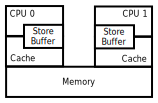
\includegraphics{advsync/SystemArchSB}}
\caption{System Architecture With Store Buffers}
\label{fig:advsync:System Architecture With Store Buffers}
\end{figure}

따라서 CPU 들은
Figure~\ref{fig:advsync:System Architecture With Store Buffers} 에 보인 것처럼
store buffer 를 장착합니다.
특정 CPU 가 특정 변수에게 해당 변수가 해당 CPU 의 캐시에 존재하지 않을 때
스토어를 행한다면, 이 새로운 값은 해당 CPU 의 store buffer 위에 위치하게
됩니다.
이 CPU 는 이제 해당 스토어가 다른 CPU 의 캐시들에 존재하는, 해당 변수의 기존
값들에 적절한 조치를 취할 때까지 기다리지 않고 곧바로 동작을 할 수 있습니다.
\iffalse

CPUs therefore come equipped with store buffers, as shown in
Figure~\ref{fig:advsync:System Architecture With Store Buffers}.
When a given CPU does a store to a given variable when that
variable is not present in that CPU's cache, then the new value
is instead placed in that CPU's store buffer.
The CPU can then proceed immediately, without having to wait for the
store to do something about all the old values of that variable
residing in other CPUs' caches.
\fi

\begin{figure}[htb]
\centering
\resizebox{3in}{!}{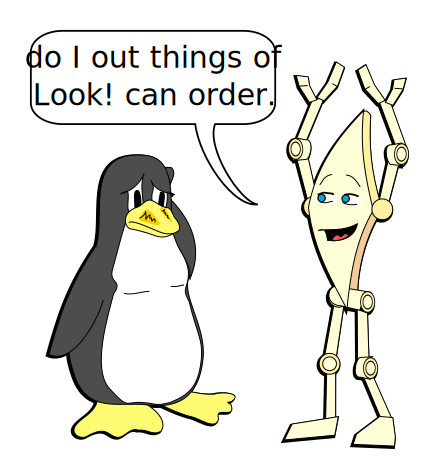
\includegraphics{cartoons/r-2014-Out-of-order}}
\caption{CPUs Can Do Things Out of Order}
\ContributedBy{Figure}{fig:advsync:CPUs Can Do Things Out of Order}{Melissa Broussard}
\end{figure}

Store buffer 들이 성능을 상당히 향상시킬 수 있긴 하지만, 이것들은
인스트럭션들과 메모리 레퍼런스들이 비순차적으로 실행될 수 있게 만들어서 결국
Figure~\ref{fig:advsync:CPUs Can Do Things Out of Order} 에 보인 것처럼 상당한
혼란을 일으킬 수 있습니다.
구체적으로, 이런 store buffer 들은
Figure~\ref{fig:advsync:Memory Misordering: Store-Buffering Litmus Test}
에 보인 store-buffering litmus test 에 보인 메모리 순서 문제를 일으킬 수
있습니다.
\iffalse

Although store buffers can greatly increase performance,
they can cause instructions and memory references to execute out
of order, which can in turn cause serious confusion, as illustrated in
Figure~\ref{fig:advsync:CPUs Can Do Things Out of Order}.
In particular, these store buffers can cause the memory misordering
shown in the store-buffering litmus test in
Figure~\ref{fig:advsync:Memory Misordering: Store-Buffering Litmus Test}.
\fi

\begin{table*}
\small
\centering\OneColumnHSpace{-.2in}
\begin{tabular}{r||l|l|l||l|l|l}
	& \multicolumn{3}{c||}{CPU 0} & \multicolumn{3}{c}{CPU 1} \\
	\cline{2-7}
	& Instruction & Store Buffer & Cache &
		Instruction & Store Buffer & Cache \\
	\hline
	\hline
	1 & (Initial state) & & \tco{x1==0} &
		(Initial state) & & \tco{x0==0} \\
	\hline
	2 & \tco{x0 = 2;} & \tco{x0==2} & \tco{x1==0} &
		\tco{x1 = 2;} & \tco{x1==2} & \tco{x0==0} \\
	\hline
	3 & \tco{r2 = x1;} (0) & \tco{x0==2} & \tco{x1==0} &
		\tco{r2 = x0;} (0) & \tco{x1==2} & \tco{x0==0} \\
	\hline
	4 & (Read-invalidate) & \tco{x0==2} & \tco{x0==0} &
		(Read-invalidate) & \tco{x1==2} & \tco{x1==0} \\
	\hline
	5 & (Finish store) & & \tco{x0==2} &
		(Finish store) & & \tco{x1==2} \\
\end{tabular}
\caption{Memory Misordering: Store-Buffering Sequence of Events}
\label{tab:advsync:Memory Misordering: Store-Buffering Sequence of Events}
\end{table*}

Table~\ref{tab:advsync:Memory Misordering: Store-Buffering Sequence of Events}
은 이 메모리 순서 문제가 어떻게 일어날 수 있는지 보입니다.
Row~1 은 초기 상태를 보이는데, CPU~0 는 \co{x1} 을 자신의 캐시에 가지고 있고
CPU~1 은 \co{x0} 를 자신의 캐시에 가지고 있으며, 두 변수들은 값 0을 갖습니다.
Row~2 는 각 CPU 의 (
Figure~\ref{fig:advsync:Memory Misordering: Store-Buffering Litmus Test} line~9
와~18 의) 스토어로 인한 상태 변화를 보입니다.
두 CPU 모두 자신의 캐시의 변수에 스토어를 하지 않았으므로, 두 CPU 모두 각자의
스토어를 각자의 store buffer 에 저장합니다.
\iffalse

Table~\ref{tab:advsync:Memory Misordering: Store-Buffering Sequence of Events}
shows how this memory misordering can happen.
Row~1 shows the initial state, where CPU~0 has \co{x1} in its cache
and CPU~1 has \co{x0} in its cache, both variables having a value of zero.
Row~2 shows the state change due to each CPU's store (lines~9 and~18 of
Figure~\ref{fig:advsync:Memory Misordering: Store-Buffering Litmus Test}).
Because neither CPU has the stored-to variable in its cache, both CPUs
record their stores in their respective store buffers.
\fi

\QuickQuiz{}
	잠깐만요!!!
	Table~\ref{tab:advsync:Memory Misordering: Store-Buffering Sequence of Events}
	의 row~2 에서 \co{x0} 와 \co{x1} 모두 각각 동시에 두개의 값, 0과 2를
	가지고 있어요.
	이게 어떻게 동작할 수 있죠???
	\iffalse

	But wait!!!
	On row~2 of
	Table~\ref{tab:advsync:Memory Misordering: Store-Buffering Sequence of Events}
	both \co{x0} and \co{x1} each have two values at the same time,
	namely zero and two.
	How can that possibly work???
	\fi
\QuickQuizAnswer{
	일을 돌아갈 수 있게 해주는 cache-coherence 프로토콜이 그 아래에 있는데,
	이에 대해선 뒤에서 설명할 겁니다.
	하지만 동시에 두개의 값을 갖는 변수가 있을 수 있다는게 놀랍다면,
	Section~\ref{sec:advsync:Variables Can Have More Than One Value} 까지
	잠깐 기다려 주세요!
	\iffalse

	There is an underlying cache-coherence protocol that straightens
	things out, which will be discussed later.
	% @@@ Add forward reference.
	But if you think that a given variable having two values at
	the same time is surprising, just wait until you get to
	Section~\ref{sec:advsync:Variables Can Have More Than One Value}!
	\fi
} \QuickQuizEnd

Row~3 는
(Figure~\ref{fig:advsync:Memory Misordering: Store-Buffering Litmus Test}
line~10 과~19 의) 두개의 읽기를 보입니다.
각 CPU 에 의해 읽혀지는 이 변수는 해당 CPU 의 캐시에 존재하므로, 각각의 읽기는
곧바로 캐시에 이쓴 값을 리턴하는데, 둘 다 0입니다.

하지만 CPU 들은 아직 일이 다 끝나지 않았습니다: 금방이든 나중이든, CPU 들은
각자의 store buffer 를 비워야만 합니다.
캐시들은 데이터를 \emph{캐시라인} 이라 불리는, 상대적으로 더 큰 블록 단위로
움직이기 때문에, 그리고 각각의 캐시라인은 여러 변수들을 담고 있을 수 있기에,
각각의 CPU 는 해당 캐시라인을 각자의 캐시에 가져와서 자신의 store buffer 에
있는 변수가 속한 캐시라인의 부분을 해당 캐시라인의 다른 부분을 망가뜨리지
않은채 업데이트 할 수 있게 해야 합니다.
각 CPU 는 또한 해당 캐시라인이 다른 CPU 의 캐시에는 없을 것을 보장해야 하는데,
read-invalidate 오퍼레이션이 이를 위해 사용됩니다.
Row~4 에 보인 것처럼, read-invalidate 오퍼레이션 두개가 모두 완료된 후에는, 두
CPU 는 캐시라인들을 거래했고, 따라서 CPU~0 의 캐시는 이제 \co{x0} 를 가지고
있고 CPU~1 의 캐시는 \co{x1} 을 가지고 있게 됩니다.
일단 이 두 변수들이 새로운 위치로 위치하게 되면, 각 CPU 는 각자의 store buffer
를 연관된 캐시라인으로 비울 수 있어서, 각 변수가 row~5 에 보인 것처럼 최종값을
가지고 있게 해줄 수 있습니다.
\iffalse

Row~3 shows the two reads (lines~10 and~19 of
Figure~\ref{fig:advsync:Memory Misordering: Store-Buffering Litmus Test}).
Because the variable being read by each CPU is in that CPU's cache,
each read immediately returns the cached value, which in both cases
is zero.

But the CPUs are not done yet: Sooner or later, they must empty their
store buffers.
Because caches move data around in relatively large blocks called
\emph{cachelines}, and because each cacheline can hold several
variables, each CPU must get the cacheline into its own cache so
that it can update the portion of that cacheline corresponding
to the variable in its store buffer, but without disturbing any
other part of the cacheline.
Each CPU must also ensure that the cacheline is not present in any other
CPU's cache, for which a read-invalidate operation is used.
As shown on row~4, after both read-invalidate operations complete,
the two CPUs have traded cachelines, so that CPU~0's cache now contains
\co{x0} and CPU~1's cache now contains \co{x1}.
Once these two variables are in their new homes, each CPU can flush
its store buffer into the corresponding cache line, leaving each
variable with its final value as shown on row~5.
\fi

\QuickQuiz{}
	하지만 이 값은 또 캐시에서 메인 메모리로 비워져야 하지 않나요?
	\iffalse

	But don't the values also need to be flushed from the cache
	to main memory?
	\fi
\QuickQuizAnswer{
	놀라운 이야기일 수 있겠으나, 꼭 그래야 하지는 않습니다!
	일부 시스템들에서는, 두 변수들이 많이 사용되면, 그 값은 CPU 의 캐시들
	사이에서 반복적으로 왔다갔다 하게 되고 메인 메모리에는 절대 돌아오지
	않습니다.
	\iffalse

	Perhaps surprisingly, not necessarily!
	On some systems,
	if the two variables are being used heavily, they might
	be bounced back and forth between the CPUs' caches and never
	land in main memory.
	\fi
} \QuickQuizEnd

요약하자면, store buffer 들은 CPU 들이 store 인스트럭션들을 효율적으로 다룰 수
있도록 하기 위해 필요하지만, 이것들은 반직관적인 메모리 순서 문제를 일으킬 수
있습니다.

하지만 여러분의 알고리즘이 정말로 순서를 지킨 메모리 레퍼런스를 필요로 한다면
뭘 해야 할까요?
결국은 \emph{메모리 배리어} (예를 들어, 리눅스 커널의 \co{smp_mb()}) 를
사용해서 순서가 지켜지는 환상을 유지할 책임을 가진 컴파일러 지시어와 표준적
동기화 도구들 (락킹과 RCU 같은) 이 있습니다.
이 메모리 배리어들은 ARM, POWER, Itanium, 그리고 Alpha 에서와 같이 명시적
인스트럭션일 수 있고, x86 에서와 같이 다른 인스트럭션들에 내포되어질 수
있습니다.
이런 표준 동기화 도구들은 순서규칙의 환상을 제공하기에, 여러분이 해야할 일은 이
도구들을 사용하는 것이므로, 이 섹션을 더이상 읽지 마시기 바랍니다.
\iffalse

In summary, store buffers are needed to allow CPUs to handle
store instructions efficiently, but they can result in
counter-intuitive memory misordering.

But what do you do if your algorithm really needs its memory
references to be ordered?
It turns out that there are compiler directives and standard
synchronization primitives (such as locking and RCU)
that are responsible for maintaining the illusion of ordering through use of
\emph{memory barriers} (for example, \co{smp_mb()} in the Linux kernel).
These memory barriers can be explicit instructions, as they are on
ARM, POWER, Itanium, and Alpha, or they can be implied by other instructions,
as they often are on x86.
Since these standard synchronization primitives preserve the illusion of
ordering, your path of least resistance is to simply use these primitives,
thus allowing you to stop reading this section.
\fi

\begin{figure}
{ \scriptsize
\begin{verbbox}
 1 C C-SB+o-mb-o+o-mb-o
 2 {
 3 }
 4
 5 P0(int *x0, int *x1)
 6 {
 7   int r2;
 8
 9   WRITE_ONCE(*x0, 2);
10   smp_mb();
11   r2 = READ_ONCE(*x1);
12 }
13
14
15 P1(int *x0, int *x1)
16 {
17   int r2;
18
19   WRITE_ONCE(*x1, 2);
20   smp_mb();
21   r2 = READ_ONCE(*x0);
22 }
23
24 exists (1:r2=0 /\ 0:r2=0)
\end{verbbox}
}
\centering
\theverbbox
\caption{Memory Ordering: Store-Buffering Litmus Test}
\label{fig:advsync:Memory Ordering: Store-Buffering Litmus Test}
\end{figure}

하지만, 여러분이 동기화 도구를 여러분 스스로 구현해야 한다면, 또는 어떻게
메모리 순서 규칙과 메모리 배리어가 동작하는지 알고 싶다면, 계속 읽으세요!
첫번째 단계는 \co{smp_mb()} 리눅스 커널 메모리 배리어가 \co{P0()} 와 \co{P1()}
의 스토어와 로드 사이에 위치한 것을 제외하고는
Figure~\ref{fig:advsync:Memory Misordering: Store-Buffering Litmus Test} 의
코드와 동일한
Figure~\ref{fig:advsync:Memory Ordering: Store-Buffering Litmus Test}
(\path{C-SB+o-mb-o+o-mb-o.litmux}) 입니다.
\iffalse

However, if you need to implement the synchronization primitives
themselves, or if you are simply interested in understanding how memory
ordering and memory barriers work, read on!
The first stop is
Figure~\ref{fig:advsync:Memory Ordering: Store-Buffering Litmus Test}
(\path{C-SB+o-mb-o+o-mb-o.litmux}),
which the \co{smp_mb()} Linux-kernel full memory barrier placed between
the store and load in both \co{P0()} and \co{P1()}, but is otherwise
identical to the code shown in
Figure~\ref{fig:advsync:Memory Misordering: Store-Buffering Litmus Test}.
\fi
% Test C-SB+o-mb-o+o-mb-o Allowed
% Histogram (3 states)
% 49553298:>0:r2=2; 1:r2=0;
% 49636449:>0:r2=0; 1:r2=2;
% 810253:>0:r2=2; 1:r2=2;
% No
이 지시어는 제 x86 랩톱에서의 100,000,000 회의 시도에도 반직관적인 결과가
나오지 않게 막아줍니다.
흥미롭게도, 이 지시어의 오버헤드는 두 로드가 모두 값 2를 리턴하는 합법적 결과가
800,000 회 넘게 발생하게 해주는데, 이는 지시어가 없는
Figure~\ref{fig:advsync:Memory Misordering: Store-Buffering Litmus Test} 의 167
회에 반대되는 결과입니다.
\iffalse

These directives prevent the counter-intuitive outcome from happening
on 100,000,000 trials on my x86 laptop.
Interestingly enough, the overhead of these directives causes the
legal outcome where both loads return the value two to happen more
than 800,000 times, as opposed to only 167 times for the
directive-free code in
Figure~\ref{fig:advsync:Memory Misordering: Store-Buffering Litmus Test}.
\fi

\begin{table*}
\small
\centering\OneColumnHSpace{-0.2in}
\begin{tabular}{r||l|l|l||l|l|l}
	& \multicolumn{3}{c||}{CPU 0} & \multicolumn{3}{c}{CPU 1} \\
	\cline{2-7}
	& Instruction & Store Buffer & Cache &
		Instruction & Store Buffer & Cache \\
	\hline
	\hline
	1 & (Initial state) & & \tco{x1==0} &
		(Initial state) & & \tco{x0==0} \\
	\hline
	2 & \tco{x0 = 2;} & \tco{x0==2} & \tco{x1==0} &
		\tco{x1 = 2;} & \tco{x1==2} & \tco{x0==0} \\
	\hline
	3 & \tco{smp_mb();} & \tco{x0==2} & \tco{x1==0} &
		\tco{smp_mb();} & \tco{x1==2} & \tco{x0==0} \\
	\hline
	4 & (Read-invalidate) & \tco{x0==2} & \tco{x0==0} &
		(Read-invalidate) & \tco{x1==2} & \tco{x1==0} \\
	\hline
	5 & (Finish store) & & \tco{x0==2} &
		(Finish store) & & \tco{x1==2} \\
	\hline
	6 & \tco{r2 = x1;} (2) & & \tco{x1==2} &
		\tco{r2 = x0;} (2) & & \tco{x0==2} \\
\end{tabular}
\caption{Memory Ordering: Store-Buffering Sequence of Events}
\label{tab:advsync:Memory Ordering: Store-Buffering Sequence of Events}
\end{table*}

이 지시어들은 순서에 대해 깊은 영향을 끼치는데, 이에 대해
Table~\ref{tab:advsync:Memory Ordering: Store-Buffering Sequence of Events}
에서 볼 수 있습니다.
Row~3 의 \co{smp_mb()} 가 상태를 바꾸지는 않지만, 이것들은 스토어가 로드 전에
완료되도록 하는데, 이는
Table~\ref{tab:advsync:Memory Misordering: Store-Buffering Sequence of Events}
에서 본 반직관적인 결과를 없앱니다.
변수 \co{x0} 와 \co{x1} 은 각각 여전히 row~2 에서 하나 이상의 값을 갖는데, 앞서
이야기 되었듯 이 지시어들은 결국은 올바른 결과를 내놓게 해줍니다.

실제 하드웨어는 여기 설명된 것보다 훨씬 더 복잡하고 교묘하다는 걸 알아두시기
바랍니다.
무엇보다도, 이 이야기의 핵심은 여러분에게 하드웨어 구조를 가르치려는게 아니라,
여러분이 저수준 동시적 기능들을 올바르게 사용하도록 돕는 겁니다.
하지만 먼저, 하나의 변수가 한 순간에 얼마나 많은 값들을 가질 수 있는지 간단히
봅시다.
\iffalse

These directives have a profound effect on ordering, as can be seen in
Table~\ref{tab:advsync:Memory Ordering: Store-Buffering Sequence of Events}.
Although the \co{smp_mb()} instructions on row~3
do not change state
in and of themselves, they do cause the stores to complete before the
loads, which rules out the counter-intuitive outcome shown in
Table~\ref{tab:advsync:Memory Misordering: Store-Buffering Sequence of Events}.
Note that variables \co{x0} and \co{x1} each still have more than one
value on row~2, however, as promised earlier, the directives straighten
things out in the end.

Please note that actual hardware tends to be much more complex, tricky,
and subtle than is described here.
After all, the point of this discussion is not to train you to be
a hardware architect, but rather to help you correctly code
low-level concurrent primitives.
But first, let's take a quick look at just how many values a single
variable might have at a single moment of time.
\fi


\subsection{Variables Can Have More Than One Value}
\label{sec:advsync:Variables Can Have More Than One Value}

변수가 잘 정의된 글로벌한 순서로 값의 시퀀스를 갖는다고 생각하는건 자연스러운
일입니다.
하지만, 지금은 안타깝더라도 이런 안락한 상상에 작별을 고해야 할 때입니다.
다행히도, 여러분은
Tables~\ref{tab:advsync:Memory Misordering: Store-Buffering Sequence of Events}
과~\ref{tab:advsync:Memory Ordering: Store-Buffering Sequence of Events} 의
row~2 로 이미 ``작별''을 고하기 시작했을 겁니다만, 어떻든, 이 섹션의 목적은 이
요점을 전달하려는 것입니다.

여기서, Figure~\ref{fig:advsync:Software Logic Analyzer} 의 코드 조각을
보기 바랍니다.
이 코드 조각은 여러 CPU 들에 의해 병렬로 실행됩니다.
Line~1 은 공유된 변수 하나를 자신의 CPU 의 ID 로 값을 넣고, line~2 에서는
몇개의 변수들을 모든 CPU 들에 동기화 되는, 세밀한 하드웨어 ``timebase``
카운터를 얻어오는 (안타깝지만, 모든 CPU 아키텍쳐에서 가능한 일은 아닙니다!)
\co{gettb()} 함수로 얻어온 값으로 초기화 하며, line~3-8 의 루프에서는 이 CPU 가
변수에 할당한 값을 통해 자신이 루프 내에서 사용한 시간의 길이를 기록합니다.
물론, CPU 들 가운데 하나만 루프에 남는데 ``승리하고'', 따라서 line~6-7 의
체크에 걸리기 전까지는지 루프를 빠져나가지 않을 것입니다.
\iffalse

It is natural to think of a variable as taking on a well-defined
sequence of values in a well-defined, global order.
Unfortunately, it is time to say ``goodbye'' to this comforting fiction.
Hopefully, you already started to say ``goodbye'' in response to row~2 of
Tables~\ref{tab:advsync:Memory Misordering: Store-Buffering Sequence of Events}
and~\ref{tab:advsync:Memory Ordering: Store-Buffering Sequence of Events},
but either way, the purpose of this section is to drive this point home.

To this end, consider the program fragment shown in
Figure~\ref{fig:advsync:Software Logic Analyzer}.
This code fragment is executed in parallel by several CPUs.
Line~1 sets a shared variable to the current CPU's ID, line~2
initializes several variables from a \co{gettb()} function that
delivers the value of a fine-grained hardware ``timebase'' counter that is
synchronized among all CPUs (not available from all CPU architectures,
unfortunately!), and the loop from lines~3-8 records the length of
time that the variable retains the value that this CPU assigned to it.
Of course, one of the CPUs will ``win'', and would thus never exit
the loop if not for the check on lines~6-7.
\fi

\QuickQuiz{}
	Figure~\ref{fig:advsync:Software Logic Analyzer} 의 코드 조각이
	가정하고 있는, 실제 하드웨어에서는 불가능한 일은 무엇인가요?
	\iffalse

	What assumption is the code fragment
	in Figure~\ref{fig:advsync:Software Logic Analyzer}
	making that might not be valid on real hardware?
	\fi
\QuickQuizAnswer{
	해당 코드는 주어진 CPU 가 자신의 값을 보는 것을 멈추는 순간, 최종의
	모든 CPU 가 동의한, 최종값을 볼 것이라 생각합니다.
	실제 하드웨어에서는, 일부 CPU 들은 마지막 값에 이르기 이전의 중간 상태
	값도 볼 수 있습니다.
	\iffalse

	The code assumes that as soon as a given CPU stops
	seeing its own value, it will immediately see the
	final agreed-upon value.
	On real hardware, some of the CPUs might well see several
	intermediate results before converging on the final value.
	\fi
} \QuickQuizEnd

\begin{figure}[tbp]
{ \scriptsize
\begin{verbbox}
  1 state.variable = mycpu;
  2 lasttb = oldtb = firsttb = gettb();
  3 while (state.variable == mycpu) {
  4   lasttb = oldtb;
  5   oldtb = gettb();
  6   if (lasttb - firsttb > 1000)
  7     break;
  8 }
\end{verbbox}
}
\centering
\theverbbox
\caption{Software Logic Analyzer}
\label{fig:advsync:Software Logic Analyzer}
\end{figure}

루프의 종료 전까지, \co{firsttb} 는 최초 할당된 값인 타임스탬프를 가지고 있게
되고 \co{lasttb} 는 이번 타임스탬프 샘플링 이전 샘플링에서 얻어져 할당되었고
여전히 변수에 담겨 있는 타임스탬프를, 또는, 해당 변수가 루프 진입 전에 바뀐 값
그대로라면, \co{firsttb} 와 동일한 값을 가지고 있을 겁니다.
이는 Figure~\ref{fig:advsync:A Variable With Multiple Simultaneous Values} 에
그려진 것처럼 532 나노세컨드의 시간동안 각 CPU 가 \co{state.variable} 을 보는
시각을 그려볼 수 있게 합니다.
이 데이터는 2006년에 각자 2개의 하드웨어 쓰레드를 갖는 8개의 코어를 갖는
1.5GHz POWER5 시스템 에서 얻어졌습니다.
CPU~1, 2, 3, 4 는 CPU~0 가 테스트를 제어하는 동안 값을 기록했습니다.
타임스탬프 카운터가 값을 증가시키는 시간은 약 5.32 ns 이었으므로, 중간의 캐시
상태를 관찰하는데 충분히 세밀했습니다.
\iffalse

Upon exit from the loop, \co{firsttb} will hold a timestamp
taken shortly after the assignment and \co{lasttb} will hold
a timestamp taken before the last sampling of the shared variable
that still retained the assigned value, or a value equal to \co{firsttb}
if the shared variable had changed before entry into the loop.
This allows us to plot each CPU's view of the value of \co{state.variable}
over a 532-nanosecond time period, as shown in
Figure~\ref{fig:advsync:A Variable With Multiple Simultaneous Values}.
This data was collected in 2006 on 1.5\,GHz POWER5 system with 8 cores,
each containing a pair of hardware threads.
CPUs~1, 2, 3, and~4 recorded the values, while CPU~0 controlled the test.
The timebase counter period was about 5.32\,ns, sufficiently fine-grained
to allow observations of intermediate cache states.
\fi

\begin{figure}[htb]
\centering
\resizebox{3in}{!}{\includegraphics{advsync/MoreThanOneValue}}
\caption{A Variable With Multiple Simultaneous Values}
\label{fig:advsync:A Variable With Multiple Simultaneous Values}
\end{figure}

각각의 수평선은 각 CPU 의 관찰 결과를 시간에 따라 나타내는데, 왼쪽의 검정색
영역은 해당 CPU 의 첫번째 관측 전의 시간을 나타냅니다.
첫 5ns 동안, CPU~3 만이 해당 변수에 대해 의견을 제시합니다.
다음 10ns 동안, CPU~2 와 3 이 해당 변수의 값에 동의하지 않지만, 곧이어 해당
값은 ``2'' 라고 동의하게 되며, 이것이 최종 동의된 값입니다.
하지만, CPU~1 은 이 값이 ``1'' 이라고 거의 300ns 동안 믿으며, CPU~4 는 거의
500ns 동안이나 해당 값이 ``4'' 라고 믿습니다.
\iffalse

Each horizontal bar represents the observations of a given CPU over time,
with the black regions to the left indicating the time before the
corresponding CPU's first measurement.
During the first 5\,ns, only CPU~3 has an opinion about the value of the
variable.
During the next 10\,ns, CPUs~2 and~3 disagree on the value of the variable,
but thereafter agree that the value is~``2'', which is in fact
the final agreed-upon value.
However, CPU~1 believes that the value is~``1'' for almost 300\,ns, and
CPU~4 believes that the value is~``4'' for almost 500\,ns.
\fi

\QuickQuiz{}
	어떻게 CPU 들이 하나의 변수에 대해 \emph{같은 시간} 에 그 값을 다르게
	볼 수 있을까요?
	\iffalse

	How could CPUs possibly have different views of the
	value of a single variable \emph{at the same time}?
	\fi
\QuickQuizAnswer{
	많은 CPU 들이 최근의 쓰기 값을 기록하며 연관된 캐시 라인이 CPU 로
	불려갈 때 적용되는 write buffer 들을 갖습니다.
	따라서, 각 CPU 가 한 변수에 대해 동시에 서로 다른 값을 보는 것이
	가능합니다 --- 그리고 메인 메모리는 또다른 값을 가지고 있을 수
	있습니다.
	메모리 배리어가 만들어진 이유들 중 하나는 소프트웨어가 이런 상황을 잘
	처리할 수 있도록 하기 위해서입니다.
	\iffalse

	Many CPUs have write buffers that record the values of
	recent writes, which are applied once the corresponding
	cache line makes its way to the CPU.
	Therefore, it is quite possible for each CPU to see a
	different value for a given variable at a single point
	in time---and for main memory to hold yet another value.
	One of the reasons that memory barriers were invented was
	to allow software to deal gracefully with situations like
	this one.
	\fi
} \QuickQuizEnd

\QuickQuiz{}
	CPU~2 와 3 은 그렇게 빨리 합의에 이르렀는데 CPU~1 과 4 는 그렇게 오래
	걸린 이유가 뭐죠?
	\iffalse

	Why do CPUs~2 and~3 come to agreement so quickly, when it
	takes so long for CPUs~1 and~4 to come to the party?
	\fi
\QuickQuizAnswer{
	CPU~2 와 3 은 같은 코어에서 수행되는 하드웨어 쓰레드여서 같은 캐시
	구조를 공유하며, 따라서 매우 적은 통신 대기시간을 갖습니다.
	이건 NUMA, 또는, 더 정확히는, NUCA 효과입니다.

	이 사실은 CPU~2 와 3 이 동의하지 않는 경우가 왜 발생할 수 있는 건지
	궁금하게 만듭니다.
	한가지 가능한 이유는 CPU~2 와 3 이 공유된 커다란 캐시 외에도 작은 개별
	캐시를 가지고 있을 수도 있다는 점입니다.
	또다른 가능한 이유는 인스트럭션 재배치로, 동의에 걸리는 시간이 매우
	짧은 10 나노세컨드라는 점과 해당 코드에 메모리 배리어가 없다는 점이 이
	가설을 뒷받침합니다.
	\iffalse

	CPUs~2 and~3 are a pair of hardware threads on the same
	core, sharing the same cache hierarchy, and therefore have
	very low communications latencies.
	This is a NUMA, or, more accurately, a NUCA effect.

	This leads to the question of why CPUs~2 and~3 ever disagree
	at all.
	One possible reason is that they each might have a small amount
	of private cache in addition to a larger shared cache.
	Another possible reason is instruction reordering, given the
	short 10-nanosecond duration of the disagreement and the
	total lack of memory barriers in the code fragment.
	\fi
} \QuickQuizEnd

그리고 네개의 CPU 만으로 이루어진 상황에 음모가 있었다고 생각한다면,
같은 상황을 보여주지만 이번에는 15개의 CPU 들이 하나의 공유 변수에 각자의 수를
$t=0$ 시간에 값 할당하는 상황을 보여주는
Figure~\ref{fig:advsync:A Variable With Multiple Simultaneous Values} 를 생각해
봅시다.
그림의 가로축은 시간 기반의 틱들로 측정된 시간을 보이는데, 그런 각각의 틱은
약 5.3 나노세컨드 정도씩 유지됩니다.
따라서 전체 이벤트의 흐름은
Figure~\ref{fig:advsync:A Variable With Multiple Simultaneous Values} 에 기록된
이벤트보다 조금은 더 길게 유지되는데, 이 텀은 CPU 수가 늘어날수록 일관적으로 더
증가합니다.
위의 다이어그램은 전체적인 그림을, 아래쪽의 다이어그램은 처음의 50개 시간 기반
틱들의 관측 결과를 확대해서 보입니다.

다시 말하지만, CPU~0 는 테스트를 관장하므로, 어떤 값도 기록하지 않습니다.
\iffalse

And if you think that the situation with four CPUs was intriguing, consider
Figure~\ref{fig:advsync:A Variable With More Simultaneous Values},
which shows the same situation, but with 15~CPUs each assigning their
number to a single shared variable at time~$t=0$. Both diagrams in the
figure are drawn in the same way as 
Figure~\ref{fig:advsync:A Variable With Multiple Simultaneous Values}.
The only difference is that the unit of horizontal axis is timebase ticks,
with each tick lasting about 5.3~nanoseconds.
The entire sequence therefore lasts a bit longer than the events recorded in
Figure~\ref{fig:advsync:A Variable With Multiple Simultaneous Values},
consistent with the increase in number of CPUs.
The upper diagram shows the overall picture, while the lower one shows
the zoom-up of first 50~timebase ticks.

Again, CPU~0 coordinates the test, so does not record any values.
\fi

\begin{figure*}
\centering
\resizebox{5in}{!}{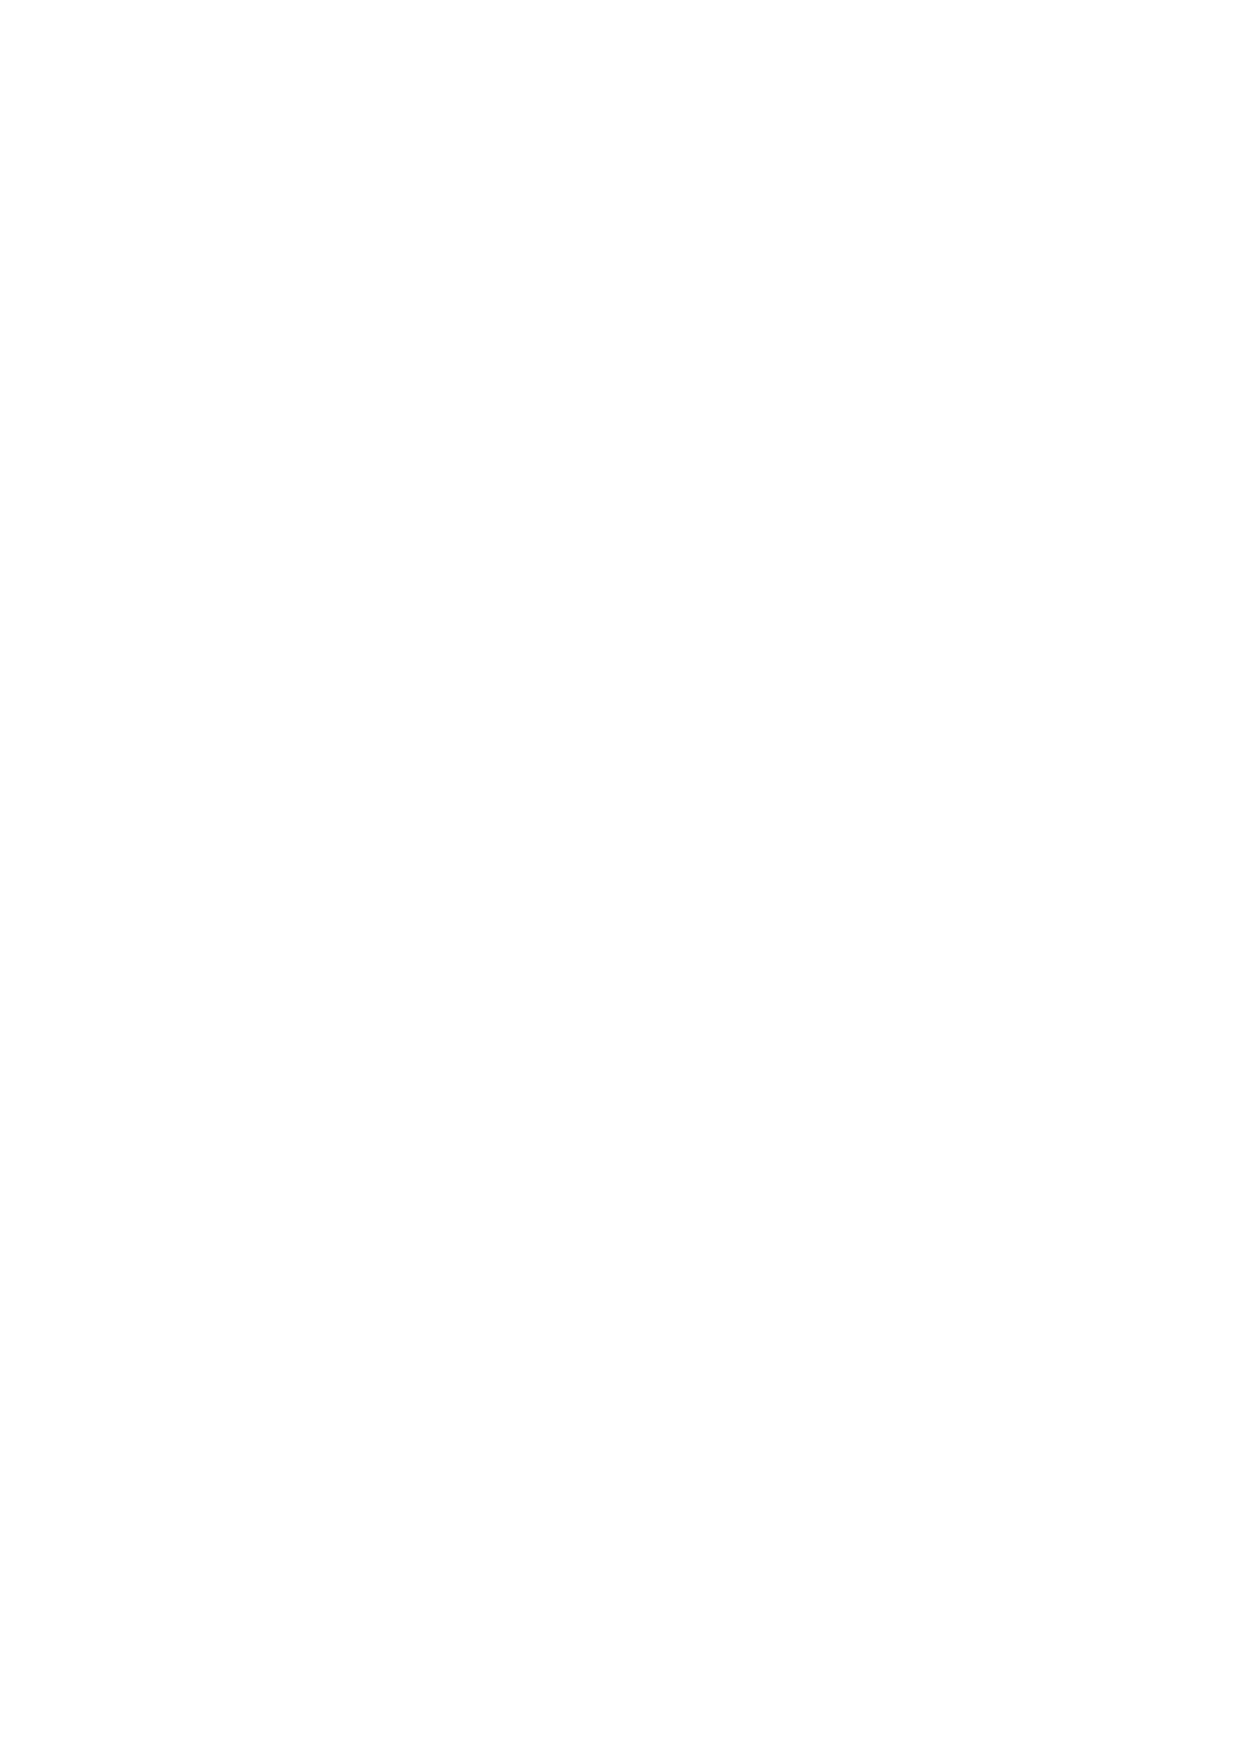
\includegraphics{advsync/MoreThanOneValue-15CPU}}
\caption{A Variable With More Simultaneous Values}
\ContributedBy{Figure}{fig:advsync:A Variable With More Simultaneous Values}{Akira Yokosawa}
\end{figure*}

모든 CPU들이 최종적으로는 마지막 값 9에 합의하게 되는데, 값 15와 12 가 전체
흐름을 주도하기 전입니다.
시간 20 에서는 해당 변수의 값에 대한 14개의 서로 다른 의견이 존재함에
유의하시기 바랍니다.
또한 모든 CPU 들이
Figure~\ref{fig:advsync:Possible Global Orders With More Simultaneous Values}
에 보여지고 있는 방향성 있는 그래프와 일관된 순서의 흐름을 보고 있음을
유의하시기 바랍니다.
더도 아니고 덜도 아니고, 이 표와 그림은 둘 다 메모리 순서에 신경 쓰는 코드에서
올바른 메모리 배리어의 사용의 중요성을 강조하고 있습니다.
\iffalse

All CPUs eventually agree on the final value of~9, but not before
the values~15 and~12 take early leads.
Note that there are fourteen different opinions on the variable's value
at time~21 indicated by the vertical line in the lower diagram.
Note also that all CPUs see sequences whose orderings are consistent with
the directed graph shown in
Figure~\ref{fig:advsync:Possible Global Orders With More Simultaneous Values}.
Nevertheless, both figures underscore the importance of
proper use of memory barriers for code that cares about memory ordering.
\fi

\begin{figure}[htb]
\centering
\resizebox{2.5in}{!}{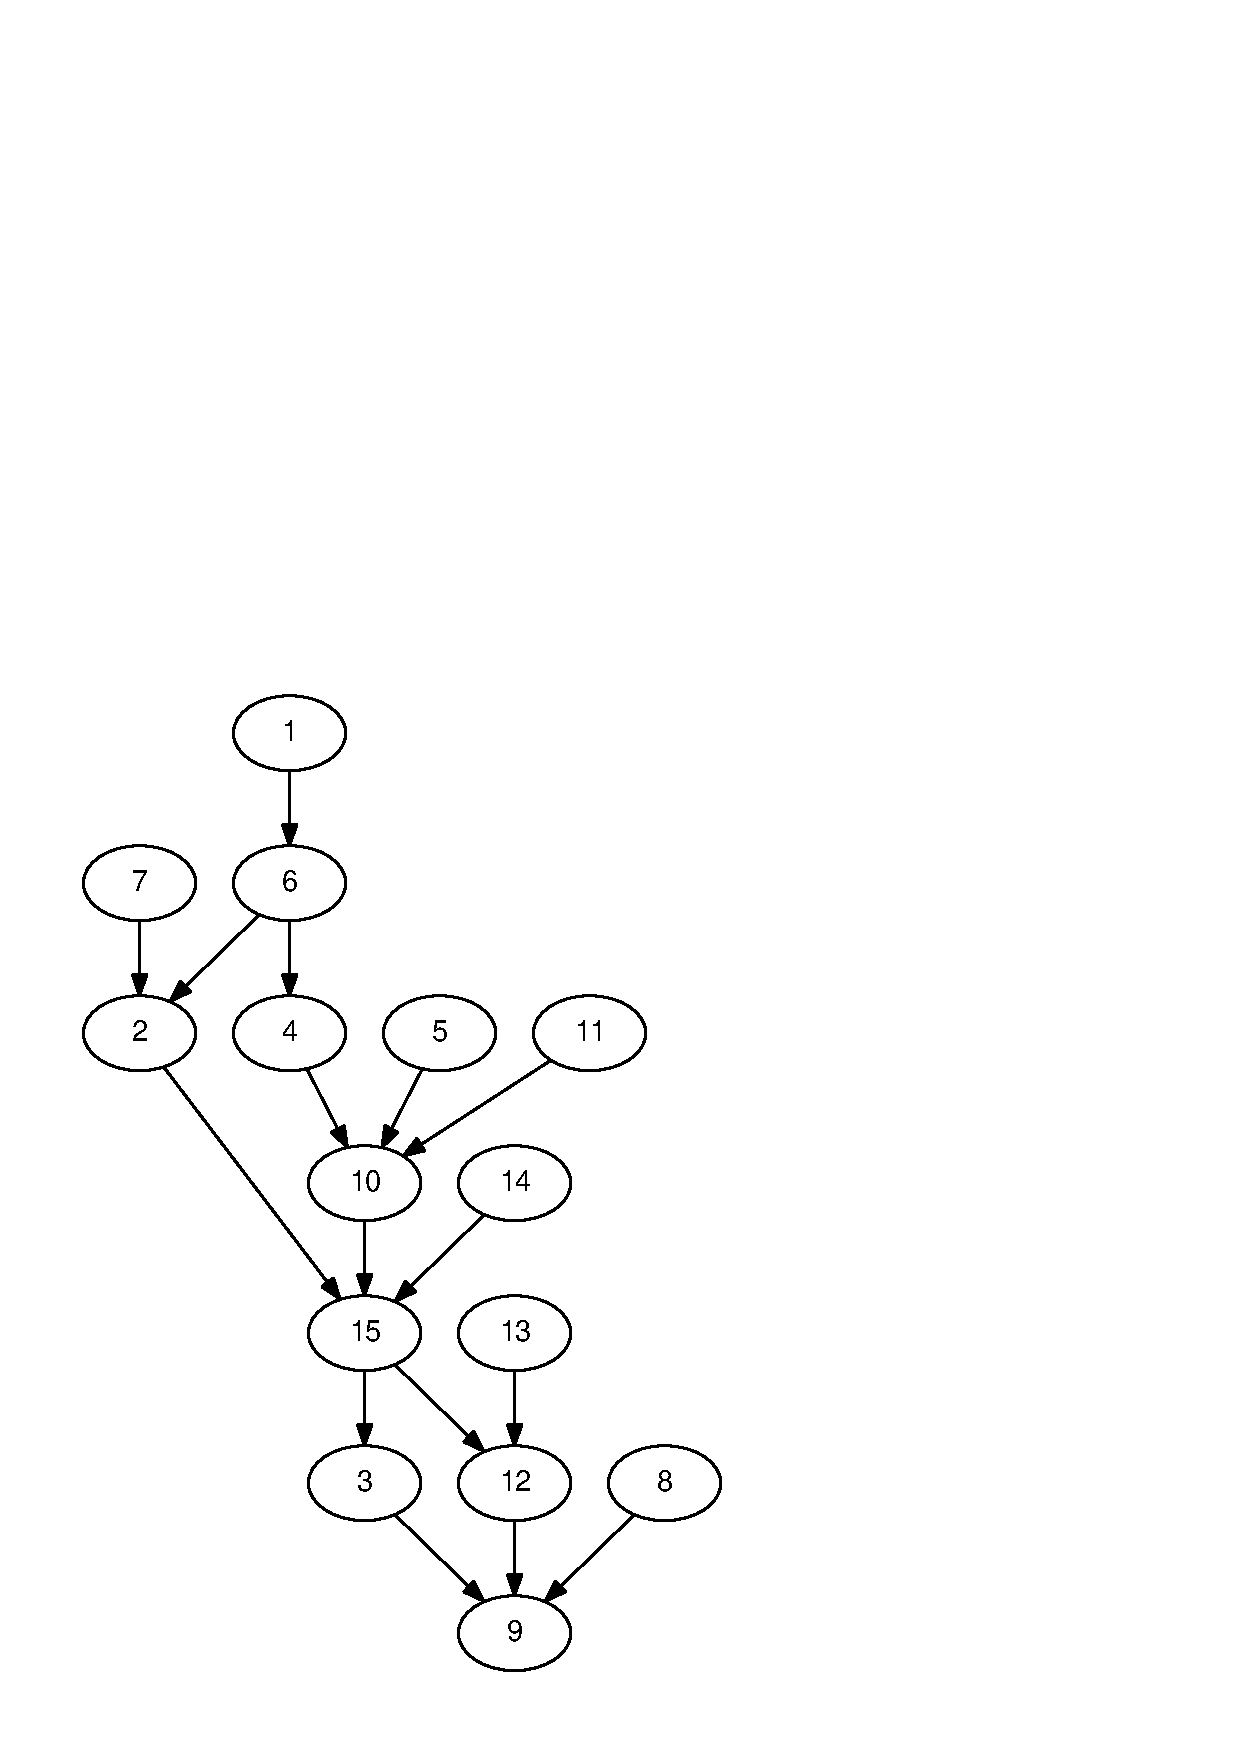
\includegraphics{advsync/store15tred}}
\caption{Possible Global Orders With More Simultaneous Values}
\label{fig:advsync:Possible Global Orders With More Simultaneous Values}
\end{figure}

시간상의 한 순간에 하나의 변수는 얼마나 많은 값들을 가질 수 있을까요?
시스템에 있는 store buffer 당 하나씩입니다!
따라서 우리는 변수의 값과 시간의 흐름에 대한 편안한 직관에 작별을 고해야 하는
정권에 들어온 것입니다.
이제 메모리 배리어가 필요해지는 체제입니다.
\iffalse

How many values can a single variable take on at a single point in
time?
As many as one per store buffer in the system!
We have therefore entered a regime where we must bid a fond farewell to
comfortable intuitions about values of variables and the passage of time.
This is the regime where memory barriers are needed.
\fi

이 모든 것과 별도로, Chapter~\ref{chp:Hardware and its Habits}
와~\ref{cha:Partitioning and Synchronization Design} 에서 얻은 교훈들을
기억하는 것이 중요합니다.
모든 CPU 들이 같은 변수에 동시적으로 값을 쓰게 하는 것은 결코 병렬 프로그램을
설계하는 방식이 아닙니다, 적어도 성능과 확장성이 전혀 중요하지 않은게 아니라면
말입니다.

불행히도, 메모리 순서규칙은 여러분의 직관을 깨트릴 수 있는 많은 방법들을 가지고
있고, 이런 방법들 모두가 성능과 확장성과 충돌하지는 않습니다.
다음 섹션은 이런 직관을 깨트리는 것들 중 일부에 대한 개관을 제공합니다.
\iffalse

All that aside, it is important to remember the lessons from
Chapters~\ref{chp:Hardware and its Habits}
and~\ref{cha:Partitioning and Synchronization Design}.
Having all CPUs write concurrently to the same variable
is absolutely no way to design a parallel program, at least
not if performance and scalability are at all important to you.

Unfortunately, memory ordering has many other ways of insulting your
intuition, and not all of these ways conflict with performance and
scalability.
The next section will give an overview of a few of these insults.
\fi

\subsection{If B Follows A, and C Follows B, Why Doesn't C Follow A?}
\label{sec:advsync:If B Follows A, and C Follows B, Why Doesn't C Follow A?}

% @@@ Replace this with WRC, RWC, or similar.
% @@@ Non-multicopy atomicity example as opposed to transitivity.

@@@ Roadmap

\subsubsection{Memory-Reference Reordering}
\label{sec:advsync:Memory-Reference Reordering}

Section~\ref{sec:advsync:Memory Ordering and Memory Barriers}
은 x86과 같이 상대적으로 강한 순서규칙의 시스템들조차도 만약 store 와 load 가
서로 다른 변수들에 가해지는 것들이라면 앞의 store 들을 뒤의 load 들과 순서 바꿀
수 있음을 보였습니다.
이 섹션은 그 결과에 기반해서, load 와 store 의 다른 조합들에 대해 알아봅니다.
\iffalse

Section~\ref{sec:advsync:Memory Ordering and Memory Barriers}
showed that even relatively strongly ordered systems like x86
can reorder prior stores with later loads, at least when the
store and load are to different variables.
This section builds on that result, looking at the other combinations of
loads and stores.
\fi

% @@@ Rationale for further reordering.

\begin{figure}[tbp]
{ \scriptsize
\begin{verbbox}
 1 C C-MP+o-wmb-o+o-o.litmus
 2
 3 {
 4 }
 5
 6
 7 P0(int* x0, int* x1) {
 8
 9   WRITE_ONCE(*x0, 2);
10   smp_wmb();
11   WRITE_ONCE(*x1, 2);
12
13 }
14
15 P1(int* x0, int* x1) {
16
17   int r2;
18   int r3;
19
20   r2 = READ_ONCE(*x0);
21   r3 = READ_ONCE(*x1);
22
23 }
24
25 exists (1:r2=2 /\ 1:r3=0)
\end{verbbox}
}
\centering
\theverbbox
\caption{Message-Passing Litmus Test}
\label{fig:advsync:Message-Passing Litmus Test}
\end{figure}

\paragraph{Load Followed By Load:}
Figure~\ref{fig:advsync:Message-Passing Litmus Test}
는 고전적인 \emph{message-passing} 리트머스 테스트를 보이는데, 여기서 \co{x0}
는 메세지이고 \co{x1} 은 메세지가 현재 있는지 없는지 알리는 flag 입니다.
이 테스트에서, \co{smp_wmb()} 는 \co{P0()} 로의 쓰기가 순서대로 이루어지도록
강제합니다만, 일기에 대해서는 어떤 순서도 명시하지 않습니다.
x86 과 같은 상대적으로 강한 순서규칙의 아키텍쳐들은 순서를 강제합니다.
하지만, 완화된 순서규칙의 아키텍쳐들은 이를 강제하지
않습니다~\cite{JadeAlglave2011ppcmem}.
\iffalse

Figure~\ref{fig:advsync:Message-Passing Litmus Test}
shows the classic \emph{message-passing} litmus test, where \co{x0} is
the message and \co{x1} is a flag indicating whether or not a message
is available.
In this test, the \co{smp_wmb()} forces \co{P0()} writes to be ordered,
but there is no ordering specified for the reads.
Relatively strongly ordered architectures, such as x86, do enforce ordering.
However, weakly ordered archictures do not necessarily enforce
this~\cite{JadeAlglave2011ppcmem}.
\fi

\begin{figure}[tbp]
{ \scriptsize
\begin{verbbox}
 1 C C-MP+o-wmb-o+o-rmb-o.litmus
 2
 3 {
 4 }
 5
 6 P0(int* x0, int* x1) {
 7
 8   WRITE_ONCE(*x0, 2);
 9   smp_wmb();
10   WRITE_ONCE(*x1, 2);
11
12 }
13
14 P1(int* x0, int* x1) {
15
16   int r2;
17   int r3;
18
19   r2 = READ_ONCE(*x1);
20   smp_rmb();
21   r3 = READ_ONCE(*x0);
22
23 }
24
25 exists (1:r2=2 /\ 1:r3=0)
\end{verbbox}
}
\centering
\theverbbox
\caption{Enforcing Order of Message-Passing Litmus Test}
\label{fig:advsync:Enforcing Order of Message-Passing Litmus Test}
\end{figure}

따라서, 이 경우의 순서규칙에 기반한 이식성 있는 코드는 예를 들면
Figure~\ref{fig:advsync:Enforcing Order of Message-Passing Litmus Test} 의
\co{smp_rmb()} 와 같은 명시적인 순서를 추가해야 합니다.
\iffalse

Therefore, portable code relying on ordering in this case should
add explicit ordering, for example, the \co{smp_rmb()} shown on
line~20 of
Figure~\ref{fig:advsync:Enforcing Order of Message-Passing Litmus Test}.
\fi

\begin{figure}[tbp]
{ \scriptsize
\begin{verbbox}
 1 C C-LB+o-o+o-o
 2 {
 3 }
 4
 5 P0(int *x0, int *x1)
 6 {
 7   int r2;
 8
 9   r2 = READ_ONCE(*x1);
10   WRITE_ONCE(*x0, 2);
11 }
12
13
14 P1(int *x0, int *x1)
15 {
16   int r2;
17
18   r2 = READ_ONCE(*x0);
19   WRITE_ONCE(*x1, 2);
20 }
21
22 exists (1:r2=2 /\ 0:r2=2)
\end{verbbox}
}
\centering
\theverbbox
\caption{Load-Buffering Litmus Test}
\label{fig:advsync:Load-Buffering Litmus Test}
\end{figure}

\paragraph{Load Followed By Store:}
Figure~\ref{fig:advsync:Load-Buffering Litmus Test}
는 고전적인 \emph{load-buffering} 리트머스 테스트를 보입니다.
x86 이나 IBM Mainframe 과 같이 상대적으로 강한 순서규칙의 시스템들은 앞의 load
를 뒤의 store 와 순서 바꾸지는 않지만, 더 약한 순서규칙의 아키텍쳐들은 정말로
그런 재배치를 합니다~\cite{JadeAlglave2011ppcmem}.
\iffalse

Figure~\ref{fig:advsync:Load-Buffering Litmus Test}
shows the classic \emph{load-buffering} litmus test.
Although relatively strongly ordered systems such as x86
or the IBM Mainframe do not reorder prior loads with subsequent stores,
more weakly ordered architectures really do allow such
reordering~\cite{JadeAlglave2011ppcmem}.
\fi

\begin{figure}[tbp]
{ \scriptsize
\begin{verbbox}
 1 C C-LB+o-r+a-o.litmus
 2 {
 3 }
 4
 5 P0(int *x0, int *x1)
 6 {
 7   int r2;
 8
 9   r2 = READ_ONCE(*x1);
10   smp_store_release(x0, 2);
11 }
12
13
14 P1(int *x0, int *x1)
15 {
16   int r2;
17
18   r2 = smp_load_acquire(x0);
19   WRITE_ONCE(*x1, 2);
20 }
21
22 exists (1:r2=2 /\ 0:r2=2)
\end{verbbox}
}
\centering
\theverbbox
\caption{Enforcing Ordering of Load-Buffering Litmus Test}
\label{fig:advsync:Enforcing Ordering of Load-Buffering Litmus Test}
\end{figure}

흥미롭게도, 실제 하드웨어가 이런 재배치를 하는 경우는 상대적으로 흔치
않습니다~\cite{LucMaranget2017aarch64}.
그렇지만, 여러분은
Figure~\ref{fig:advsync:Enforcing Ordering of Load-Buffering Litmus Test} 에
예로 든 것과 같이 모든 필요한 순서규칙을 강제해야 합니다.
\iffalse

Interestingly enough, it is relatively rare for actual hardware to
exhibit this reordering~\cite{LucMaranget2017aarch64}.
Nevertheless, you should enforce any required ordering, for example,
as shown in
Figure~\ref{fig:advsync:Enforcing Ordering of Load-Buffering Litmus Test}.
\fi

\begin{figure}[tbp]
{ \scriptsize
\begin{verbbox}
 1 C C-MP+o-o+o-rmb-o.litmus
 2
 3 {
 4 }
 5
 6 P0(int* x0, int* x1) {
 7
 8   WRITE_ONCE(*x0, 2);
 9   WRITE_ONCE(*x1, 2);
10
11 }
12
13 P1(int* x0, int* x1) {
14
15   int r2;
16   int r3;
17
18   r2 = READ_ONCE(*x1);
19   smp_rmb();
20   r3 = READ_ONCE(*x0);
21
22 }
23
24 exists (1:r2=2 /\ 1:r3=0)
\end{verbbox}
}
\centering
\theverbbox
\caption{Message-Passing Litmus Test, No Writer Ordering}
\label{fig:advsync:Message-Passing Litmus Test, No Writer Ordering}
\end{figure}

\paragraph{Store Followed By Store:}
Figure~\ref{fig:advsync:Message-Passing Litmus Test, No Writer Ordering}
는 한번 더 고전적 message-passing 리트머스 테스트를 보입니다만, 이번엔
\co{P0()} 의 쓰기들에 대한 명시적 순서규칙이 없고, \co{P1()} 의 읽기들에 대한
순서규칙을 \co{smp_mb()} 로 제공하고 있습니다.
다시 말하지만, 상대적으로 강한 순서규칙의 아키텍쳐들은 순서를 강제합니다만,
완화된 순서규칙의 아키텍쳐들은 그러지 않습니다~\cite{JadeAlglave2011ppcmem}.
따라서, 이식성 있는 코드는
Figure~\ref{fig:advsync:Enforcing Order of Message-Passing Litmus Test} 에 예를
든 것과 같이 쓰기들에 대해 명시적으로 순서를 잡아줘야 합니다.
\iffalse

Figure~\ref{fig:advsync:Message-Passing Litmus Test, No Writer Ordering}
once again shows the classic message-passing litmus test, but without
explicit ordering for \co{P0()}'s writes and with the \co{smp_mb()}
providing ordering for \co{P1()}'s reads.
Again, the relatively strongly ordered architectures do enforce ordering,
but weakly ordered architectures do not necessarily do
so~\cite{JadeAlglave2011ppcmem}.
Therefore, portable code should explicitly order the writes, for
example, as shown in
Figure~\ref{fig:advsync:Enforcing Order of Message-Passing Litmus Test}.
\fi

\subsubsection{Address Dependencies}
\label{sec:advsync:Address Dependencies}

Address dependency 는 load 인스트럭션으로 리턴받은 값이 뒤의 메모리 레퍼런스
인스트럭션에 사용되는 주소를 계산하는데 사용될 때 발생합니다.
\iffalse

An address dependency occurs when the value returned by a load instruction
is used to compute the address used by a later memory-reference
instruction.
\fi

\begin{figure}[tbp]
{ \scriptsize
\begin{verbbox}
 1 C C-MP+o-wmb-o+o-ad-o.litmus
 2
 3 {
 4 int y=1;
 5 int *x1 = &y;
 6 }
 7
 8 P0(int* x0, int** x1) {
 9
10   WRITE_ONCE(*x0, 2);
11   smp_wmb();
12   WRITE_ONCE(*x1, x0);
13
14 }
15
16 P1(int** x1) {
17
18   int *r2;
19   int r3;
20
21   r2 = READ_ONCE(*x1);
22   r3 = READ_ONCE(*r2);
23
24 }
25
26 exists (1:r2=x0 /\ 1:r3=1)
\end{verbbox}
}
\centering
\theverbbox
\caption{Message-Passing Address-Dependency Litmus Test}
\label{fig:advsync:Message-Passing Address-Dependency Litmus Test}
\end{figure}

Figure~\ref{fig:advsync:Message-Passing Address-Dependency Litmus Test}
는 message-passing 패턴의 link 를 사용한 변종을 보입니다.
여기서 head pointer 는 \co{x1} 으로, 초기에 \co{int} 변수 \co{y} 를 레퍼런스
(line~5) 하며, 이 변수는 초기에 값 $1$ 로 초기화 됩니다 (line~4).

\co{P0()} 는 head pointer \co{x1} 이 \co{x0} 를 레퍼런스 하도록 업데이트
(line~12) 하지만 이는 \co{x0} 를 $2$ 로 초기화 (line~10) 하고 순서를 강제
(line~11) 한 후입니다.
\co{P1()} 은 head pointer \co{x1} 을 읽어오고 (line~21), 이어서 이 포인터가
레퍼런스 하는 값을 읽어옵니다 (line~22).
따라서 line~21 의 로드에서 line~22 의 로드로의 address dependency 가
존재합니다.
이 경우에는 line~21 의 로드에 의해 리턴되는 값이 곧바로 line~22 의 로드에
사용되는 주소인데, C-언어의 \co{->} 오퍼레이터, 더하기, 빼기, 배열 인덱싱 등을
사용한 필드 접근 등의 여러 다른 형태가 존재할 수 있습니다.

Line~21 의 head pointer 로부터의 로드가 line~22 의 dereference 앞으로 순서가
지켜지기를 바랄 수 있습니다.
하지만, DEC Alpha 의 경우에는
Section~\ref{sec:app:whymb:Alpha}
에서 더 자세히 설명하는대로 여기서의 종속성 있는 읽기에 예측된 값을 사용할 수도
있기에 그렇지 않습니다.
\iffalse

Figure~\ref{fig:advsync:Message-Passing Address-Dependency Litmus Test}
shows a linked variant of the message-passing pattern.
The head pointer is \co{x1}, which initially
references the \co{int} variable \co{y} (line~5), which is in turn 
initialized to the value $1$ (line~4).

\co{P0()} updates head pointer \co{x1} to reference \co{x0} (line~12),
but only afer initializing it to $2$ (line~10) and forcing ordering
(line~11).
\co{P1()} picks up the head pointer \co{x1} (line~21), and then loads
the referenced value (line~22).
There is thus an address dependency from the load on line~21 to the
load on line~22.
In this case, the value return by the load on line~21 is exactly the address
used by the load on line~22, but many variations are possible,
including field access using the C-language \co{->} operator,
addition, subtraction, and array indexing.

One might hope that line~21's load from the head pointer would be ordered
before line~22's dereference.
However, this is not the case on DEC Alpha, which can in effect use
a speculated value for the dependent read, as described in more detail in
Section~\ref{sec:app:whymb:Alpha}.
\fi

\begin{figure}[tbp]
{ \scriptsize
\begin{verbbox}
 1 C C-MP+o-wmb-o+ld-ad-o.litmus
 2
 3 {
 4 int y=1;
 5 int *x1 = &y;
 6 }
 7
 8 P0(int* x0, int** x1) {
 9
10   WRITE_ONCE(*x0, 2);
11   smp_wmb();
12   WRITE_ONCE(*x1, x0);
13
14 }
15
16 P1(int** x1) {
17
18   int *r2;
19   int r3;
20
21   r2 = lockless_dereference(*x1);
22   r3 = READ_ONCE(*r2);
23
24 }
25
26 exists (1:r2=x0 /\ 1:r3=1)
\end{verbbox}
}
\centering
\theverbbox
\caption{Enforced Ordering of Message-Passing Address-Dependency Litmus Test}
\label{fig:advsync:Enforced Ordering of Message-Passing Address-Dependency Litmus Test}
\end{figure}

Figure~\ref{fig:advsync:Enforced Ordering of Message-Passing Address-Dependency Litmus Test}
는 line~21 의 \co{READ_ONCE()} 를 \co{lockless_dereference()} 로 교체함으로써
DEC Alpha 조차 포함해서 제대로 동작하고 이식성 있는 코드를 어떻게 만들 수
있는지 보이는데, \co{lockless_dereference()} 는 DEC Alpha 외의 모든
플랫폼에서는 \co{READ_ONCE()} 처럼 동작하고, DEC Alpha 에서는 \co{READ_ONCE()}
에 이어 \co{smp_mb()} 가 이어지는 것처럼 동작해서 모든 플랫폼에서 필요한
순서규칙을 강제합니다.
\iffalse

Figure~\ref{fig:advsync:Enforced Ordering of Message-Passing Address-Dependency Litmus Test}
shows how to make this work portably, even on DEC Alpha, by
replacing line~21's \co{READ_ONCE()} with \co{lockless_dereference()},
which acts like \co{READ_ONCE()} on all platforms other than DEC Alpha,
where it acts like a \co{READ_ONCE()} followed by an \co{smp_mb()},
thereby forcing the required ordering on all platforms.
\fi

\begin{figure}[tbp]
{ \scriptsize
\begin{verbbox}
 1 C C-S+o-wmb-o+o-ad-o.litmus
 2
 3 {
 4 int y=1;
 5 int *x1 = &y;
 6 }
 7
 8 P0(int* x0, int** x1) {
 9
10   WRITE_ONCE(*x0, 2);
11   smp_wmb();
12   WRITE_ONCE(*x1, x0);
13
14 }
15
16 P1(int** x1) {
17
18   int *r2;
19
20   r2 = READ_ONCE(*x1);
21   WRITE_ONCE(*r2, 3);
22
23 }
24
25 exists (1:r2=x0 /\ x0=2)
\end{verbbox}
}
\centering
\theverbbox
\caption{S Address-Dependency Litmus Test}
\label{fig:advsync:S Address-Dependency Litmus Test}
\end{figure}

하지만
Figure~\ref{fig:advsync:S Address-Dependency Litmus Test}
에 보인 \emph{S} 리트머스 테스트~\cite{JadeAlglave2011ppcmem} 처럼
이 종속적 오퍼레이션이 읽기가 아니라 쓰기라 가정해 봅시다.
어떤 제품 품질의 아키텍쳐도 쓰기를 예측적으로 하진 않기에 line~10 의
\co{WRITE_ONCE()} 가 line~21 의 \co{WRITE_ONCE()} 를 덮어쓰지는 않을 것이어서
line~25 의 \co{exists} 절은 종속적 읽기의 경우에 필요했던
\co{lockless_dereference()} 없이도 DEC Alpha 에서조차도 만족될 수 없을
것입니다.
\iffalse

But suppose that the dependent operation is a write rather than
a read, for example, in the \emph{S}
litmus test~\cite{JadeAlglave2011ppcmem} shown in
Figure~\ref{fig:advsync:S Address-Dependency Litmus Test}?
Because no production-quality architecture speculated writes,
it is not possible for the \co{WRITE_ONCE()} on line~10 to overwrite
the \co{WRITE_ONCE()} on line~21, meaning that the \co{exists}
clause on line~25 cannot be satisfied, even on DEC Alpha, even
without the \co{lockless_dereference()} that is required in the
dependent-read case.
\fi

하지만, address dependicy 들은
Section~\ref{sec:advsync:Address- and Data-Dependency Restrictions}
에서 이야기하듯 컴파일러 최적화에 의해 쉽게 깨질 수 있습니다는 점을 알아두시기
바랍니다.
\iffalse

However, it is important to note that address dependencies can
be fragile and easily broken by compiler optimizations, as discussed in
Section~\ref{sec:advsync:Address- and Data-Dependency Restrictions}.
\fi

\subsubsection{Data Dependencies}
\label{sec:advsync:Data Reordering}

% @@@ More details on how hardware deals with address and data
% @@@ dependencies
% @@@ Explain hardware tagging of dependencies.

\subsubsection{Control Dependencies}
\label{sec:advsync:Control Dependencies}

\subsubsection{Non-Multicopy Atomicity}
\label{sec:advsync:Non-Multicopy Atomicity}

\subsubsection{Non-Single-Copy Atomicity}
\label{sec:advsync:Non-Single-Copy Atomicity}

메모리 순서 규칙과 메모리 배리어는 매우 비직관적일 수 있습니다.
예를 들어, Figure~\ref{fig:advsync:Parallel Hardware is Non-Causal} 의 함수들이
변수 A, B, C 가 초기값 0을 가진 채 병렬로 수행되는 경우를 생각해보세요:
\iffalse

Memory ordering and memory barriers can be extremely counter-intuitive.
For example, consider the functions shown in
Figure~\ref{fig:advsync:Parallel Hardware is Non-Causal}
executing in parallel
where variables~A, B, and~C are initially zero:
\fi

\begin{figure}[htbp]
{ \scriptsize
\begin{verbbox}
  1 thread0(void)
  2 {
  3   A = 1;
  4   smp_wmb();
  5   B = 1;
  6 }
  7
  8 thread1(void)
  9 {
 10   while (B != 1)
 11     continue;
 12   barrier();
 13   C = 1;
 14 }
 15
 16 thread2(void)
 17 {
 18   while (C != 1)
 19     continue;
 20   barrier();
 21   assert(A != 0);
 22 }
\end{verbbox}
}
\centering
\theverbbox
\caption{Parallel Hardware is Non-Causal}
\label{fig:advsync:Parallel Hardware is Non-Causal}
\end{figure}

직관적으로 볼 때, \co{thread0()} 는 B 의 값 할당을 A 에의 값 할당 후에 하고,
\co{thread1()} 은 C 에 값을 할당하기 전, \co{thread0()} 가 B 에 값을 할당할
때까지 기다리며, \co{thread2()} 는 A 의 값을 보기 전에 \co{thread1()} 이 C 에
값을 할당하기까지 기다립니다.
따라서, 역시 직관적으로, line~21 의 단정문은 실패할 수 없습니다.
\iffalse

Intuitively, \co{thread0()} assigns to~B after it assigns to~A,
\co{thread1()} waits until \co{thread0()} has assigned to~B before
assigning to~C, and \co{thread2()} waits until \co{thread1()} has
assigned to~C before referencing~A.
Therefore, again intuitively, the assertion on line~21 cannot possibly
fire.
\fi

이 말은, 직관적이기는 하지만, 완전히 잘못된 것입니다.
이건 이론적인 단정이 아님에 주의하시기 바랍니다: 실제로 이 코드를 현실의 약한
순서 규칙의 하드웨어 (1.5 GHz 16-CPU POWER 5 시스템) 에서 수행하면 천만번의
수행 중 16번 이 단정문이 실패했습니다.
분명, 명시적 메모리 배리어를 사용하는 코드를 작성하는 사람은 반드시 극단적인
테스트를 해야만 합니다 -- 정확성 증명이 도움이 될 수는 있지만, 메모리 배리어의
본질적으로 비직관적인 동작은 그런 증명이 기반하는 가정을 상당히 제약할 수
있습니다.
여러개의 하드웨어 의존적인 트릭들이 이 수행에서의 실패 가능성을 상당히
\emph{증가시키기} 때문에 극단적 테스트의 필요성은 결코 가벼워질 수 없습니다.
\iffalse

This line of reasoning, intuitively obvious though it may be, is completely
and utterly incorrect.
Please note that this is \emph{not} a theoretical assertion:
actually running this code on real-world weakly-ordered hardware
(a 1.5\,GHz 16-CPU POWER 5 system) resulted in the assertion firing
16~times out of 10~million runs.
Clearly, anyone who produces code with explicit memory barriers
should do some extreme testing---although a proof of correctness might
be helpful, the strongly counter-intuitive nature of the behavior of
memory barriers should in turn strongly limit one's trust in such proofs.
The requirement for extreme testing should not be taken lightly, given
that a number of dirty hardware-dependent tricks were used to
greatly \emph{increase} the probability of failure in this run.
\fi

\QuickQuiz{}
	page~\pageref{fig:advsync:Parallel Hardware is Non-Causal} 의
	Figure~\ref{fig:advsync:Parallel Hardware is Non-Causal} 코드의 line~21
	의 단정문이 대체 어떻게 실패할 수 \emph{있죠}?
	\iffalse

	How on earth could the assertion on line~21 of the code in
	Figure~\ref{fig:advsync:Parallel Hardware is Non-Causal} on
	page~\pageref{fig:advsync:Parallel Hardware is Non-Causal}
	\emph{possibly} fail?
	\fi
\QuickQuizAnswer{
	핵심 포인트는, 직관적 분석이 놓친 것은 C 에의 값 할당 결과가 A 에의 값
	할당보다 먼저 {\tt thread2()} 에게 전파되는 것을 막는 것이 없다는
	점입니다.
	이건 이 섹션의 뒤에서 설명됩니다.
	\iffalse

	The key point is that the intuitive analysis missed is that
	there is nothing preventing the assignment to~C from overtaking
	the assignment to~A as both race to reach \co{thread2()}.
	This is explained in the remainder of this section.
	\fi
} \QuickQuizEnd

\QuickQuiz{}
	좋아요\ldots 그래서 이걸 어떻게 고쳐야 하죠?
	\iffalse

	Great \ldots So how do I fix it?
	\fi
\QuickQuizAnswer{
	가장 쉬운 방법은 line~12 와 line~20 의 \co{barrier()} 를 \co{smp_mb()}
	로 바꾸는 것입니다.

	물론, 일부 하드웨어는 다른 하드웨어보다 너그럽습니다.
	예를 들어, x86 에서
	page~\pageref{fig:advsync:Parallel Hardware is Non-Causal}
	Figure~\ref{fig:advsync:Parallel Hardware is Non-Causal} 의 line~21 의
	단정문은 실패하지 않습니다.
	PowerPC 에서는 line~20 의 \co{barrier()} 만 \co{smp_mb()} 로 바꿔도
	단정문이 실패하지 않게 할 수 있습니다.
	\iffalse

	The easiest fix is to replace each of the \co{barrier()}s on
	line~12 and line~20 with an \co{smp_mb()}.

	Of course, some hardware is more forgiving than other hardware.
	For example, on x86 the assertion on line~21 of
	Figure~\ref{fig:advsync:Parallel Hardware is Non-Causal} on
	page~\pageref{fig:advsync:Parallel Hardware is Non-Causal}
	cannot trigger.
	On PowerPC, only the \co{barrier()} on line~20 need be
	replaced with \co{smp_mb()} to prevent the assertion from
	triggering.
	\fi
} \QuickQuizEnd

그러니 이제 어떡해야 할까요?
최선의 선택지는, 가능하다면 모든 필요한 메모리 배리어를 내포하고 있는 현존하는
기능들을 사용하고 이 챕터의 나머지 내용을 그냥 무시하는 것입니다.

물론, 동기화 도구를 직접 구현하고 있다면 그럴 수는 없습니다.
다음의 메모리 순서 규칙과 메모리 배리어에 대한 이야기는 그런 경우를 위한
것입니다.
\iffalse

So what should you do?
Your best strategy, if possible, is to use existing primitives that
incorporate any needed memory barriers, so that you can simply ignore
the rest of this chapter.

Of course, if you are implementing synchronization primitives,
you don't have this luxury.
The following discussion of memory ordering and memory barriers
is for you.
\fi

Memory ordering and memory barriers can be extremely counter-intuitive.
For example, consider the functions shown in
Figure~\ref{fig:advsync:Parallel Hardware is Non-Causal}
executing in parallel
where variables~A, B, and~C are initially zero:

% TODO: Translate this section
\iffalse
\begin{figure}[tbp]
{ \scriptsize
\begin{verbbox}
  1 thread0(void)
  2 {
  3   A = 1;
  4   smp_wmb();
  5   B = 1;
  6 }
  7
  8 thread1(void)
  9 {
 10   while (B != 1)
 11     continue;
 12   barrier();
 13   C = 1;
 14 }
 15
 16 thread2(void)
 17 {
 18   while (C != 1)
 19     continue;
 20   barrier();
 21   assert(A != 0);
 22 }
\end{verbbox}
}
\centering
\theverbbox
\caption{Parallel Hardware is Non-Causal}
\label{fig:advsync:Parallel Hardware is Non-Causal}
\end{figure}
\fi

Intuitively, \co{thread0()} assigns to~B after it assigns to~A,
\co{thread1()} waits until \co{thread0()} has assigned to~B before
assigning to~C, and \co{thread2()} waits until \co{thread1()} has
assigned to~C before referencing~A.
Therefore, again intuitively, the assertion on line~21 cannot possibly
fire.

This line of reasoning, intuitively obvious though it may be, is completely
and utterly incorrect.
Please note that this is \emph{not} a theoretical assertion:
actually running this code on real-world weakly-ordered hardware
(a 1.5\,GHz 16-CPU POWER 5 system) resulted in the assertion firing
16~times out of 10~million runs.
Clearly, anyone who produces code with explicit memory barriers
should do some extreme testing---although a proof of correctness might
be helpful, the strongly counter-intuitive nature of the behavior of
memory barriers should in turn strongly limit one's trust in such proofs.
The requirement for extreme testing should not be taken lightly, given
that a number of dirty hardware-dependent tricks were used to
greatly \emph{increase} the probability of failure in this run.

\QuickQuiz{}
	How on earth could the assertion on line~21 of the code in
	Figure~\ref{fig:advsync:Parallel Hardware is Non-Causal} on
	page~\pageref{fig:advsync:Parallel Hardware is Non-Causal}
	\emph{possibly} fail?
\QuickQuizAnswer{
	The key point is that the intuitive analysis missed is that
	there is nothing preventing the assignment to~C from overtaking
	the assignment to~A as both race to reach \co{thread2()}.
	This is explained in the remainder of this section.
} \QuickQuizEnd

\QuickQuiz{}
	Great \ldots So how do I fix it?
\QuickQuizAnswer{
	The easiest fix is to replace each of the \co{barrier()}s on
	line~12 and line~20 with an \co{smp_mb()}.

	Of course, some hardware is more forgiving than other hardware.
	For example, on x86 the assertion on line~21 of
	Figure~\ref{fig:advsync:Parallel Hardware is Non-Causal} on
	page~\pageref{fig:advsync:Parallel Hardware is Non-Causal}
	cannot trigger.
	On PowerPC, only the \co{barrier()} on line~20 need be
	replaced with \co{smp_mb()} to prevent the assertion from
	triggering.
} \QuickQuizEnd

So what should you do?
Your best strategy, if possible, is to use existing primitives that
incorporate any needed memory barriers, so that you can simply ignore
the rest of this chapter.

Of course, if you are implementing synchronization primitives,
you don't have this luxury.
The following discussion of memory ordering and memory barriers
is for you.

\subsection{What Can You Trust?}
\label{sec:advsync:What Can You Trust?}

당신은 결코 당신의 직관을 믿어선 안됩니다.

당신은 무엇을 믿을 수 \emph{있는} 걸까요?
\iffalse

You most definitely cannot trust your intuition.

What \emph{can} you trust?
\fi

당신이 메모리 배리어를 잘 사용할 수 있게 해주는 몇개의 적당히 간단한 규칙들이
있다는 게 밝혀졌습니다.
이 섹션에서는 적어도 이식성 있는 코드의 관점에서 메모리 배리어 이야기의 바닥에
도달해 보고자 하는 사람들을 위해 그런 규칙들을 유도해 봅니다.
실제 유도를 고생스럽게 해보기보다는 그냥 그 규칙들을 간단히 보고 싶다면, 부담
갖지 말고 Section~\ref{sec:advsync:A Few Simple Rules} 로 건너뛰어도 좋습니다.

메모리 배리어의 실제 개념은 CPU 에 따라 상당히 다르기 때문에 호환성 있는 코드는
메모리 배리어 개념들 중 최소한의 공통 분모들에만 의존성을 가져야 합니다.
\iffalse

It turns out that there are a few reasonably simple rules that
allow you to make good use of memory barriers.
This section derives those rules, for those who wish to get
to the bottom of the memory-barrier story, at least from the viewpoint
of portable code.
If you just want to be told what the rules are rather than suffering
through the actual derivation,
please feel free to skip to Section~\ref{sec:advsync:A Few Simple Rules}.

The exact semantics of memory barriers vary wildly from one CPU family to
another, so portable code must rely only on the least-common-denominator
semantics of memory barriers.
\fi

다행히도, 모든 CPU 들이 다음의 규칙들을 갖습니다:
\begin{enumerate}
\item	한 CPU 에 의한 모든 액세스들은 그 CPU 에는 프로그램 순서대로 일어나는
	것으로 보인다.
\item	모든 CPU 들의 하나의 변수로의 액세스들은 그 변수로의 스토어
	오퍼레이션들의 어떤 글로벌 순서 규칙에 맞춰 일관성을 갖는다.
\item	메모리 배리어들은 짝을 맞춰 동작한다.
\item	오퍼레이션들은 배타적 락킹 도구들이 구현되는 곳에 사용될 수 있다.
\end{enumerate}
\iffalse

Fortunately, all CPU families impose the following rules:
\begin{enumerate}
\item	All accesses by a given CPU will appear to that CPU to have
	occurred in program order.
\item	All CPUs' accesses to a single variable will be consistent with
	some global ordering of stores to that variable.
\item	Memory barriers will operate in a pair-wise fashion.
\item	Operations will be provided from which exclusive locking
	primitives may be constructed.
\end{enumerate}
\fi

따라서, 당신이 이식 가능한 코드에서 메모리 배리어를 사용해야 한다면, 이런
특성들에 의존할 수 있습니다.\footnote{
	또는, 아예 명시적인 메모리 배리어의 사용을 하지 않는게 나을 수도
	있습니다.
	하지만 그 방법은 다른 섹션의 주제가 될것입니다.}
이런 특성들 각각은 다음의 섹션들에서 설명됩니다.
\iffalse

Therefore, if you need to use memory barriers in portable code,
you can rely on all of these properties.\footnote{
	Or, better yet, you can avoid explicit use of memory barriers
	entirely.
	But that would be the subject of other sections.}
Each of these properties is described in the following sections.
\fi

\subsubsection{Self-References Are Ordered}

하나의 CPU 는 자신의 메모리 액세스들을 마치 인스트럭션들을 재배치나 예측성 수행
없이 한번에 하나의 인스트럭션만을 순차적으로 실행하듯이, ``프로그램 순서'' 대로
일어나는 것처럼 보게 됩니다.
오래된 CPU 들의 경우, 이 제약은 바이너리 호환성을 위해 필요하며, 우리의 타입의
소프트웨어들의 정상성은 부차적인 이유일 뿐입니다.
이 규칙을 제한된 범위 내에서나마 위반한 CPU 들도 일부 있었습니다만, 그런
경우에도 컴파일러에게 순서 규칙이 명시적으로 지켜질 수 있도록 해야 할 의무가
지워져 있었습니다.

어떤 쪽이건, 프로그래머의 관점에서 CPU 는 자신의 액세스들은 프로그램 순서대로
보게 됩니다.
\iffalse

A given CPU will see its own accesses as occurring in ``program order'',
as if the CPU was executing only one instruction at a time with no
reordering or speculation.
For older CPU families, this restriction is necessary for binary compatibility,
and only secondarily for the sanity of us software types.
There have been a few CPU families that violate this rule to a limited extent,
but in those cases, the compiler has been responsible
for ensuring that ordering is explicitly enforced as needed.

Either way, from the programmer's viewpoint, the CPU sees its own accesses
in program order.
\fi

\subsubsection{Single-Variable Memory Consistency}
\label{sec:advsync:Single-Variable Memory Consistency}

현재의 상용 컴퓨터 시스템들은 \emph{캐시 일관성} 을 제공하기 때문에, 어떤 CPU
무리가 모두 하나의 변수에 동시에 어토믹하지 않은 스토어를 하게 되면, 모든 CPU
들에 보이는 일련의 값들은 적어도 하나의 글로벌 순서 규칙에 의해 일관적일
것입니다.
예를 들어,
Figure~\ref{fig:advsync:A Variable With Multiple Simultaneous Values} 에 보이는
일련의 액세스들에서,
CPU~1 는 {\tt \{1,2\}} 순서로,
CPU~2 는 {\tt \{2\}} 순서로,
CPU~3 는 {\tt \{3,2\}} 순서로,
그리고
CPU~4 는 {\tt \{4,2\}} 순서로 그 값을 보게 됩니다.
이는 글로벌한 순서 {\tt \{3,1,4,2\}} 로 일관성을 갖습니다만, 꼭 이 순서가
아니라도 이 네개의 숫자를 가지고 ``2'' 로 끝나는, 다른 다섯개의 순서로 글로벌
순서를 유추하는 것도 가능합니다.
즉, 하나의 변수에서 얻어지는 값의 순서에는 모호함이 있긴 하나, 모든 CPU 의
합의가 이뤄집니다.
\iffalse

Because current commercially available computer systems provide
\emph{cache coherence},
if a group of CPUs all do concurrent non-atomic stores to a single variable,
the series of values seen by all CPUs will be consistent with at
least one global ordering.
For example, in the series of accesses shown in
Figure~\ref{fig:advsync:A Variable With Multiple Simultaneous Values},
CPU~1 sees the sequence {\tt \{1,2\}},
CPU~2 sees the sequence {\tt \{2\}},
CPU~3 sees the sequence {\tt \{3,2\}},
and
CPU~4 sees the sequence {\tt \{4,2\}}.
This is consistent with the global sequence {\tt \{3,1,4,2\}},
but also with all five of the other sequences of these four numbers that end
in~``2''.
Thus, there will be agreement on the sequence of values taken on
by a single variable, but there might be ambiguity.
\fi

반면에, 이 CPU 들이 간단한 유일값의 스토어가 아니라 (리눅스 커널의
\co{atomic_inc_return()} 과 같은) 어토믹 오퍼레이션들을 사용했다면, CPU 들이
보게 되는 결과들은 하나의 전체적으로 일관된 순서의 값들이 될 것입니다.
\co{atomic_inc_return()} 실행 중 하나가 먼저 일어나서 그 값을 0 에서 1 로
바꾸고, 다음엔 두번째가 1 에서 2로, 그리고 그렇게 진행됩니다.
이 CPU 들은 각자 본 것들을 비교하고 \co{atomic_inc_return()} 실행의 분명한
순서에의 합의를 얻을 수 있을 것입니다.
이는 앞서 설명한 어토믹하지 않은 스토어로는 불가능한 일인데, 어토믹하지 않은
스토어는 모호성의 가능성으로 인해 이전의 값에 대한 정보를 알려주지 않기
때문입니다.
\iffalse

In contrast, had the CPUs used atomic operations (such as the Linux kernel's
\co{atomic_inc_return()} primitive) rather than simple stores of
unique values, their observations would
be guaranteed to determine a single globally consistent sequence of values.
One of the \co{atomic_inc_return()} invocations would happen first,
and would change the value from~0 to~1, the second from~1 to~2, and
so on.
The CPUs could compare notes afterwards and come to agreement on the
exact ordering of the sequence of \co{atomic_inc_return()} invocations.
This does not work for the non-atomic stores described earlier because
the non-atomic stores do not return any indication of the earlier value,
hence the possibility of ambiguity.
\fi

이 섹션은 모든 CPU 들이 하나의 변수에 접근할 때에\emph{만} 적용됨에
주의하십시오.
이 단일 변수의 경우, 과감한 컴파일러 최적화가 리눅스 커널의 \co{ACCESS_ONCE()}
지시어나 C++11 의 완화된 어토믹 오퍼레이션들~\cite{PeteBecker2011N3242}를 통해
방지되었다는 최소한의 가정 위에서는 캐시 일관성이 글로벌한 순서를 보장합니다.
반면, 만약 여러 변수들이 있다면, 현재의 상용 컴퓨터 시스템들에서는 CPU 들이
일관성 있게 순서에 합의할 수 있도록 하기 위해 메모리 배리어가 필요합니다.
\iffalse

Please note well that this section applies \emph{only} when all
CPUs' accesses are to one single variable.
In this single-variable case, cache coherence guarantees the
global ordering, at least assuming that some of the more aggressive
compiler optimizations are disabled via the Linux kernel's
\co{READ_ONCE()} and \co{WRITE_ONCE()} directives or C++11's relaxed
atomics~\cite{PeteBecker2011N3242}.
In contrast, if there are multiple variables, memory barriers are
required for the CPUs to consistently agree on the order for current
commercially available computer systems.
\fi

\subsubsection{Pair-Wise Memory Barriers}

짝을 맞추는 메모리 배리어들은 조건적 순서 개념을 제공합니다.
예를 들어, 다음의 오퍼레이션들에 대해, 외부에서 로직 분석을 하는 쪽의
관점에서는 CPU~1 의 A 로의 액세스가 조건 없이 B 로의 액세스를 앞서지는 않습니다
\IfInBook{예를 위해 (Appendix~\ref{chp:app:whymb:Why Memory Barriers?}를
	  참고하세요)
	  }.
	  {(시스템은 그저 이 액세스들이 순서대로 이루어지는 \emph{것처럼}
	  동작할 뿐입니다; 실제로 순서대로 이루어지도록 강제될 이유는
	  없습니다).}
하지만, 만약 CPU~2 의 B 로의 액세스가 CPU~1 의 B 로의 액세스의 결과를 보게
된다면, CPU~2 의 A 로의 액세스는 CPU~1 의 A 로의 액세스의 결과 역시 보게 될
것이 보장됩니다.
일부 CPU 의 메모리 배리어들은 실은 좀 더 강력한, 무조건적 순서 개념을
제공하지만, 이식성 있는 코드는 이와 같이 좀 더 약한 조건적 순서 개념만을
사용해야 할 것입니다.
\iffalse

Pair-wise memory barriers provide conditional ordering semantics.
For example, in the following set of operations, CPU~1's access to
A does not unconditionally precede its access to~B from the viewpoint
of an external logic analyzer
\IfInBook{(see Appendix~\ref{chp:app:whymb:Why Memory Barriers?}
	  for examples)
	 }.
	 {(the system is only to act \emph{as if} the accesses
	  are in order; it is not necessarily required to actually
	  force them to be in order).}
However, if CPU~2's access to~B sees the result of CPU~1's access
to~B, then CPU~2's access to~A is guaranteed to see the result of
CPU~1's access to~A.
Although some CPU families' memory barriers do in fact provide stronger,
unconditional ordering guarantees, portable code may rely only
on this weaker if-then conditional ordering guarantee.
\fi

\vspace{5pt}
\begin{minipage}[t]{\columnwidth}
\tt
\scriptsize
\begin{tabular}{l|l}
	\nf{CPU 1}	& \nf{CPU 2} \\
	\hline
	<access> A	& <access> B \\
	<memory barrier>& <memory barrier> \\
	<access> B	& <access> A \\
\end{tabular}
\end{minipage}
\vspace{5pt}

\QuickQuiz{}
	하지만 메모리 배리어들이 무조건적으로 순서를 강제해 주지 않는다면,
	디바이스 드라이버는 대체 어떻게 안정적으로 MMIO 레지스터로의 일련의
	로드와 스토어들을 실행할 수 있나요?
	\iffalse

	But if the memory barriers do not unconditionally force
	ordering, how the heck can a device driver reliably execute
	sequences of loads and stores to MMIO registers?
	\fi
\QuickQuizAnswer{
	MMIO 레지스터들은 특별한 경우입니다: 그것들은 물리 메모리의 캐시되지
	않는 영역에 위치합니다.
	메모리 배리어들은 캐시되지 않는 메모리로의 로드와 스토어는 무조건적으로
	순서를 강제하는데, 이에 대해선 Section~\ref{sec:advsync:Device
	Operations} 에서 다루겠습니다.
	\iffalse

	MMIO registers are special cases: because they appear
	in uncached regions of physical memory.
	Memory barriers \emph{do} unconditionally force ordering
	of loads and stores to uncached memory, as discussed in
	Section~\ref{sec:advsync:Device Operations}.
	\fi
} \QuickQuizEnd

물론, 액세스들은 로드 또는 스토어야만 하고, 이것들은 서로 다른 특성을 갖습니다.
Table~\ref{tab:advsync:Memory-Barrier Combinations} 은 한 쌍의 CPU 에서 모든
가능한 로드와 스토어 조합을 보입니다.
당연하게도, 조건적 순서를 강제하기 위해, 각 CPU 의 오퍼레이션들에 짝을 맞춰
메모리 배리어를 사용해야만 합니다.
\iffalse

Of course, accesses must be either loads or stores, and these
do have different properties.
Table~\ref{tab:advsync:Memory-Barrier Combinations}
shows all possible combinations of loads and stores from a pair
of CPUs.
Of course, to enforce conditional ordering, there must be
a memory barrier between each CPU's pair of operations.
\fi

\begin{table*}
\small
\centering
\begin{tabular}{r||c|c||c|c||l}
	\multicolumn{1}{c||}{} & \multicolumn{2}{c||}{CPU 1} &
		\multicolumn{2}{c||}{CPU 2} & Description \\
	\hline
	\hline
	0 & load(A) & load(B) & load(B) & load(A) &
		Ears to ears. \\
	1 & load(A) & load(B) & load(B) & store(A) &
		Only one store. \\
	2 & load(A) & load(B) & store(B) & load(A) &
		Only one store. \\
	3 & load(A) & load(B) & store(B) & store(A) &
		Pairing 1. \\
	\hline
	4 & load(A) & store(B) & load(B) & load(A) &
		Only one store. \\
	5 & load(A) & store(B) & load(B) & store(A) &
		Pairing 2. \\
	6 & load(A) & store(B) & store(B) & load(A) &
		Mouth to mouth, ear to ear. \\
	7 & load(A) & store(B) & store(B) & store(A) &
		Pairing 3. \\
	\hline
	8 & store(A) & load(B) & load(B) & load(A) &
		Only one store. \\
	9 & store(A) & load(B) & load(B) & store(A) &
		Mouth to mouth, ear to ear. \\
	A & store(A) & load(B) & store(B) & load(A) &
		Ears to mouths. \\
	B & store(A) & load(B) & store(B) & store(A) &
		Stores ``pass in the night''. \\
	\hline
	C & store(A) & store(B) & load(B) & load(A) &
		Pairing 1. \\
	D & store(A) & store(B) & load(B) & store(A) &
		Pairing 3. \\
	E & store(A) & store(B) & store(B) & load(A) &
		Stores ``pass in the night''. \\
	F & store(A) & store(B) & store(B) & store(A) &
		Stores ``pass in the night''. \\
\end{tabular}
\caption{Memory-Barrier Combinations}
\label{tab:advsync:Memory-Barrier Combinations}
\end{table*}

\subsubsection{Pair-Wise Memory Barriers: Portable Combinations}

아래에 Table~\ref{tab:advsync:Memory-Barrier Combinations} 에서 이식성 있는
소프트웨어가 사용해야 할 모든 메모리 배리어 조합을 나열합니다.
\iffalse

The following pairings from
Table~\ref{tab:advsync:Memory-Barrier Combinations},
enumerate all the combinations of memory-barrier
pairings that portable software may depend on.
\fi

\paragraph{Pairing 1.}
	이 조합에서는, 다음과 같이 하나의 CPU 가 메모리 배리어가 중간에 위치한
	한 쌍의 로드를 실행하고, 그동안 두번째 CPU 는 역시 메모리 배리어가
	중간에 위치한 한 쌍의 스토어를 실행합니다 (A 와 B 둘 다 처음엔 0 값을
	갖습니다):
	\iffalse

	In this pairing, one CPU executes a pair of loads separated
	by a memory barrier, while a second CPU executes a pair
	of stores also separated by a memory barrier, as follows
	(both~A and~B are initially equal to zero):
	\fi

	\vspace{5pt}
	\begin{minipage}[t]{\columnwidth}
	\tt
	\scriptsize
	\begin{tabular}{l|l}
		\nf{CPU 1}	& \nf{CPU 2} \\
		\hline
		STORE A = 1	& Y = LOAD B \\
		<memory barrier>& <memory barrier> \\
		STORE B = 1	& X = LOAD A \\
	\end{tabular}
	\end{minipage}
	\vspace{5pt}

	두 CPU 모두 이 코드의 수행을 완료한 후에는, 만약 \co{Y==1} 이라면
	반드시 \co{X==1} 이어야 합니다.
	이 경우, \co{Y==1} 은 CPU~2 의, 자신의 메모리 배리어 이전의 로드가
	CPU~1 의 메모리 배리어 후의 스토어를 봤다는 뜻입니다.
	메모리 배리어 짝맞추기의 원리에 의해, CPU~2 의, 자신의 메모리 배리어
	뒤의 로드는 CPU~1 의 메모리 배리어 전의 스토어를 볼 수 있어야 하므로,
	\co{X==1} 입니다.

	반면, 만약 \co{Y==0} 라면, 메모리 배리어 조건이 잡히지 않으므로, 이
	경우 X 는 0이 될수도, 1이 될 수도 있습니다.
	\iffalse

	After both CPUs have completed executing these code sequences,
	if \co{Y==1}, then we must also have \co{X==1}.
	In this case, the fact that \co{Y==1} means that
	CPU~2's load prior to its memory barrier has
	seen the store following CPU~1's memory barrier.
	Due to the pairwise nature of memory barriers, CPU~2's
	load following its memory barrier must therefore see
	the store that precedes CPU~1's memory barrier, so that
	\co{X==1}.

	On the other hand, if \co{Y==0}, the memory-barrier condition
	does not hold, and so in this case, X~could be either~0 or~1.
	\fi

\paragraph{Pairing 2.}
	이 조합에서, 각 CPU 는 다음과 같이 로드와 메모리 배리어, 그리고
	스토어를 순서대로 실행합니다 (A 와 B 는 처음에는 0 값을 갖습니다):
	\iffalse

	In this pairing, each CPU executes a load followed by a
	memory barrier followed by a store, as follows
	(both~A and~B are initially equal to zero):
	\fi

	\vspace{5pt}
	\begin{minipage}[t]{\columnwidth}
	\tt
	\scriptsize
	\begin{tabular}{l|l}
		\nf{CPU 1}	& \nf{CPU 2} \\
		\hline
		X = LOAD A	& Y = LOAD B \\
		<memory barrier>& <memory barrier> \\
		STORE B = 1	& STORE A = 1 \\
	\end{tabular}
	\end{minipage}
	\vspace{5pt}

	두 CPU 모두 이 코드의 실행을 완료한 후, 만약 \co{X==1} 이라면 \co{Y==0}
	이어야만 합니다.
	이 경우, \co{X==1} 이라는 결과는 CPU~1 의, 자신의 메모리 배리어 전의
	로드는 CPU~2 의 메모리 배리어 후의 스토어를 봤다는 의미입니다.
	메모리 배리어 짝맞추기의 원리에 의해, CPU~1의, 자신의 메모리 배리어
	뒤의 스토어는 CPU~2 의, 자신의 메모리 배리어 앞의 로드의 결과를 봐야
	하므로, \co{Y==0} 이어야 합니다.

	반면, 만약 \co{X==0} 라면, 메모리 배리어 조건은 성립되지 않으므로, 이
	경우 Y 의 값은 0일 수도, 1일 수도 있습니다.

	이 두 CPU 의 코드는 동일하므로, 두 CPU 모두 코드 실행을 마무리 한 후에
	\co{Y==1} 라면 \co{X==0} 일 겁니다.
	\iffalse

	After both CPUs have completed executing these code sequences,
	if \co{X==1}, then we must also have \co{Y==0}.
	In this case, the fact that \co{X==1} means that
	CPU~1's load prior to its memory barrier has
	seen the store following CPU~2's memory barrier.
	Due to the pairwise nature of memory barriers, CPU~1's
	store following its memory barrier must therefore see
	the results of CPU~2's load preceding its memory barrier,
	so that \co{Y==0}.

	On the other hand, if \co{X==0}, the memory-barrier condition
	does not hold, and so in this case, Y~could be either~0 or~1.

	The two CPUs' code sequences are symmetric, so if \co{Y==1}
	after both CPUs have finished executing these code sequences,
	then we must have \co{X==0}.
	\fi

\paragraph{Pairing 3.}
	이 조합에서는 다음과 같이 한 CPU 는 로드, 메모리 배리어, 스토어를
	순서대로 실행하고, 다른 CPU 는 메모리 배리어를 가운데 두고 두개의
	스토어를 실행합니다 (A 와 B 모두 초기값은 0입니다):
	\iffalse

	In this pairing, one CPU executes a load followed by a
	memory barrier followed by a store, while the other CPU
	executes a pair of stores separated by a memory barrier,
	as follows (both~A and~B are initially equal to zero):
	\fi

	\vspace{5pt}
	\begin{minipage}[t]{\columnwidth}
	\tt
	\scriptsize
	\begin{tabular}{l|l}
		\nf{CPU 1}	& \nf{CPU 2} \\
		\hline
		X = LOAD A	& STORE B = 2 \\
		<memory barrier>& <memory barrier> \\
		STORE B = 1	& STORE A = 1 \\
	\end{tabular}
	\end{minipage}
	\vspace{5pt}

	두 CPU 모두 코드 실행을 완료한 후, 만약 \co{X==1} 이라면, \co{B==1}
	이어야 합니다.
	이 경우, \co{X==1} 은 CPU~1 의, 자신의 메모리 배리어 앞의 로드가 CPU~2
	의 메모리 배리어 뒤의 스토어를 봤다는 의미입니다.
	메모리 배리어 짝 맞추기의 원리에 의해, CPU~1 의, 자신의 메모리 배리어
	뒤의 스토어는 CPU~2 의, 자신의 메모리 배리어 앞의 스토어의 결과를
	봐야만 합니다.
	이는 CPU~1 의 B 에의 스토어는 CPU~2 의 B 에의 스토어를 덮어써서
	\co{B==1}이 됨을 뜻합니다.

	반면, 만약 \co{X==0} 라면, 메모리 배리어 조건은 성립되지 않고, 따라서 B
	의 값은 1도, 2도 될 수 있습니다.
	\iffalse

	After both CPUs have completed executing these code sequences,
	if \co{X==1}, then we must also have \co{B==1}.
	In this case, the fact that \co{X==1} means that
	CPU~1's load prior to its memory barrier has
	seen the store following CPU~2's memory barrier.
	Due to the pairwise nature of memory barriers, CPU~1's
	store following its memory barrier must therefore see
	the results of CPU~2's store preceding its memory barrier.
	This means that CPU~1's store to~B will overwrite CPU~2's
	store to~B, resulting in \co{B==1}.

	On the other hand, if \co{X==0}, the memory-barrier condition
	does not hold, and so in this case, B~could be either~1 or~2.
	\fi

\subsubsection{Pair-Wise Memory Barriers: Semi-Portable Combinations}

Table~\ref{tab:advsync:Memory-Barrier Combinations} 에서 가져온 다음의 조합들은
최신 하드웨어에서 사용될 수 있습니다만, 1900년대에 만들어진 일부 시스템에서는
문제가 있을 수 있습니다.
하지만, 2000년 이후 소개된 모든 주류 하드웨어에서는 안전하게 사용될 수
있습니다.
그러니 메모리 배리어가 다루기 어렵다고 생각하신다면, 일부 시스템에는 \emph{더}
어렵단 점을 기억해 두시기 바랍니다!
\iffalse

The following pairings from
Table~\ref{tab:advsync:Memory-Barrier Combinations}
can be used on modern hardware, but might fail on some systems
that were produced in the 1900s.
However, these \emph{can} safely be used on all mainstream hardware
introduced since the year 2000.
So if you think that memory barriers are difficult to deal with, please
keep in mind that they used to be a \emph{lot} harder on some systems!
\fi

\paragraph{Ears to Mouths.}
	스토어들은 로드들의 결과를 볼 수 없기에(다시 말하지만, MMIO 레지스터는
	지금 당장은 잊어주시기 바랍니다), 메모리 배리어 조건이 맞춰졌는지를
	항상 알 수는 없습니다.
	하지만, 21-세기 하드웨어는 적어도 로드들 중 하나는 연관된 스토어에 의해
	저장된 값을 봤다고 보장해줄 수도 있습니다 (또는 같은 변수에 대한 뒤의
	값을).
	\iffalse

	Since the stores cannot see the results of the loads
	(again, ignoring MMIO registers for the moment),
	it is not always possible to determine whether the memory-barrier
	condition has been met.
	However, 21\textsuperscript{st}-century
	hardware \emph{would} guarantee that at least one
	of the loads saw the value stored by the corresponding store
	(or some later value for that same variable).
	\fi

\QuickQuiz{}
	ears-to-mouths 시나리오에서 최신 하드웨어가 로드들 중 최소 하나는 다른
	쓰레드에 의해 저장된 값을 읽을 거라 보장함을 우리는 어떻게 알죠?
	\iffalse

	How do we know that modern hardware guarantees that at least
	one of the loads will see the value stored by the other thread
	in the ears-to-mouths scenario?
	\fi
\QuickQuizAnswer{
	그 시나리오는 A 와 B 의 초기값이 0이라는 가정 하에 다음과 같습니다:
	\iffalse

	The scenario is as follows, with~A and~B both initially zero:
	\fi

	\vspace{5pt}
	\begin{minipage}[t]{\columnwidth}
	\tt
	\scriptsize
	\begin{tabular}{l|l}
		\nf{CPU 0}	& \nf{CPU 1} \\
		\hline
		STORE A = 1	& STORE B = 1 \\
		<memory barrier>& <memory barrier> \\
		r1 = LOAD B	& r2 = LOAD A \\
	\end{tabular}
	\end{minipage}
	\vspace{5pt}

	두 로드 모두 관련된 스토어를 보지 못한다면, 두 CPU 들이 모두 실행을
	마쳤을 때, \co{r1} 과 \co{r2} 둘 다 0일 겁니다.
	이제 \co{r1} 이 0이라고 생각해 봅시다.
	그렇다면 CPU~0 의 B 로부터의 로드가 CPU~1 의 B 로의 스토어 이전에
	일어났음을 알 수 있습니다: 그렇지 않다면 \co{r1} 이 1일 겁니다.
	하지만 CPU~0 의 B 로부터의 로드가 CPU~1 의 B 로의 스토어 이전에
	일어났으므로, 메모리 배리어 조합이 CPU~0 의 A 로의 스토어가 CPU~1 의 A
	로부터의 로드 이전에 일어났음을 보장하고, 따라서 \co{r2} 는 0이 아니라
	1일 것임을 보장합니다.

	따라서, \co{r1} 과 \co{r2} 중 하나는 0이 아닐 것이고, 이는 이야기 했듯
	최소 하나의 로드는 관련된 스토어를 봤음을 의미합니다.
	\iffalse

	If neither of the loads see the corresponding store, when both
	CPUs finish, both \co{r1} and \co{r2} will be equal to zero.
	Let's suppose that \co{r1} is equal to zero.
	Then we know that CPU~0's load from~B happened before CPU~1's
	store to~B: After all, we would have had \co{r1} equal to one
	otherwise.
	But given that CPU~0's load from~B happened before CPU~1's store
	to~B, memory-barrier pairing guarantees that CPU~0's store to~A
	happens before CPU~1's load from~A, which in turn guarantees that
	\co{r2} will be equal to one, not zero.

	Therefore, at least one of \co{r1} and \co{r2} must be nonzero,
	which means that at least one of the loads saw the value from
	the corresponding store, as claimed.
	\fi
} \QuickQuizEnd

\paragraph{Stores ``Pass in the Night''.}
	다음의 예에서, 두 CPU 들이 모두 코드 실행을 끝낸 후,
	{\tt \{A==1,B==2\}} 로 결론이 나는 일은 결코 없을 것처럼 보입니다.
	\iffalse

	In the following example, after both CPUs have finished
	executing their code sequences, it is quite tempting to
	conclude that the result {\tt \{A==1,B==2\}} cannot happen.
	\fi

	\vspace{5pt}
	\begin{minipage}[t]{\columnwidth}
	\tt
	\scriptsize
	\begin{tabular}{l|l}
		\nf{CPU 1}	& \nf{CPU 2} \\
		\hline
		STORE A = 1	& STORE B = 2 \\
		<memory barrier>& <memory barrier> \\
		STORE B = 1	& STORE A = 2 \\
	\end{tabular}
	\end{minipage}
	\vspace{5pt}

	안타깝게도, 이 결론은 21-세기의 시스템들에서는 맞지만, 모든 20-세기
	시스템들에서는 맞지 않을 수 있습니다.
	A 를 담고 있는 캐시 라인이 처음에는 CPU~2 에 의해 소유되고 있었고, B 를
	담는 캐시 라인은 처음에는 CPU~1 에 의해 소유되고 있었다고 생각해
	봅시다.
	그리고 나서, 무효화 큐와 스토어 버퍼를 가지고 있는 시스템들에서는,
	첫번째 값 할당이 ``밤에 지나가는 것 (pass in the night)'' 이 가능해서,
	두번째 값 할당이 실제로는 먼저 일어날 수 있습니다.
	\IfInBook{이 이상한 효과는
		  Appendix~\ref{chp:app:whymb:Why Memory Barriers?} 에서
		  설명됩니다.
		  }
	{}
	\iffalse

	Unfortunately, although this conclusion is correct on
	21\textsuperscript{st}-century systems, it does not necessarily hold
	on all antique 20\textsuperscript{th}-century systems.
	Suppose that the cache line containing~A is initially owned
	by CPU~2, and that containing~B is initially owned by CPU~1.
	Then, in systems that have invalidation queues and store
	buffers, it is possible for the first assignments to ``pass
	in the night'', so that the second assignments actually
	happen first.
	\IfInBook{This strange effect is explained in
	          Appendix~\ref{chp:app:whymb:Why Memory Barriers?}.
		 }
		 {}
	\fi

	이와 똑같은 효과는 ``ears to mouths'' 조합을 포함해, 각 CPU 의 메모리
	배리어를 스토어가 앞서는 어떤 메모리 배리어 조합에서도 발생할 수
	있습니다.

	하지만, 21-세기 하드웨어는 이런 순서 규칙을 허용하지 \emph{않아서},
	이런 조합이 안전하게 사용될 수 있도록 합니다.
	\iffalse

	This same effect can happen in any memory-barrier pairing
	where each CPU's memory barrier is preceded by a store,
	including the ``ears to mouths'' pairing.

	However, 21\textsuperscript{st}-century hardware \emph{does}
	accommodate these ordering intuitions, and \emph{do} permit
	this combination to be used safely.
	\fi

\subsubsection{Pair-Wise Memory Barriers: Dubious Combinations}

Table~\ref{tab:advsync:Memory-Barrier Combinations} 에서 가져온 다음의
조합들에서 메모리 배리어들은 21-세기 하드웨어에서도 이식성 있는 코드에서는 매우
제한적인 사용만 가능합니다. 
하지만 ``제한적인 사용'' 은 ``사용 불가'' 와는 다르니, 뭐가 가능한지 한번
봅시다!
열심인 독자분들은 이게 어떻게 동작하는지 완전히 이해하기 위해 이 조합들 각각을
사용하는 테스트용 프로그램을 작성하고자 할 것입니다.
\iffalse

In the following combinations from
Table~\ref{tab:advsync:Memory-Barrier Combinations},
the memory barriers have very limited use in portable code, even
on 21\textsuperscript{st}-century hardware.
However, ``limited use'' is different than ``no use'', so let's see
what can be done!
Avid readers will want to write toy programs that rely on each of
these combinations in order to fully understand how this works.
\fi

\paragraph{Ears to Ears.}
	로드들은 메모리의 상태를 바꾸지 않기 때문에 (MMIO 레지스터는 당장은
	무시합시다), 로드들 중 하나가 다른 로드의 결과를 볼 수는 없습니다.
	하지만, 만약 우리가 CPU~2 의 B 로부터의 로드가 CPU~1 의 B 로부터의
	로드보다 새로운 값을 리턴했음을 안다면, 우리는 CPU~2 의 A 로부터의
	로드가 CPU~1 의 A 로부터의 로드와 같거나 그보다 나중의 값을 리턴했음
	역시 알 수 있습니다.
	\iffalse

	Since loads do not change the state of memory
	(ignoring MMIO registers for the moment),
	it is not possible for one of the loads to see the
	results of the other load.
	However, if we know that CPU~2's load from~B returned a
	newer value than CPU~1's load from~B, then we also know
	that CPU~2's load from~A returned either the same value
	as CPU~1's load from~A or some later value.
	\fi

\paragraph{Mouth to Mouth, Ear to Ear.}
	변수들 중 하나는 로드되었고, 다른 하나는 스토어 되었습니다.
	로드가 다른 로드의 결과를 보는 것은 불가능하므로 (다시 말하지만, MMIO
	레지스터는 무시합니다), 메모리 배리어로 제공되는 조건적 순서를 파악할
	수는 없습니다.

	하지만, 어떤 스토어가 마지막으로 발생했는지는 알 수 있습니다만, 이를
	위해서는 B 로부터의 추가적인 로드가 필요합니다.
	이 추가적인 B 로부터의 로드가 CPU~1 과 CPU~2 가 완료된 후 수행된다면,
	그리고 그 수행으로 인해 CPU~2 의 B 로의 스토어가 마지막으로
	이루어졌음이 밝혀진다면, CPU~2 의 A 로부터의 로드는 CPU~1 의 A 로부터의
	로드와 같거나 나중의 값을 리턴했음 역시 알 수 있습니다.
	\iffalse

	One of the variables is only loaded from, and the other
	is only stored to.
	Because (once again, ignoring MMIO registers) it is not
	possible for one load to see the results of the other,
	it is not possible to detect the conditional ordering
	provided by the memory barrier.

	However, it is possible to determine which store happened
	last, but this requires an additional load from~B.
	If this additional load from~B is executed after both
	CPUs~1 and~2 complete, and if it turns out that CPU~2's
	store to~B happened last, then we know
	that CPU~2's load from~A returned either the same value
	as CPU~1's load from~A or some later value.
	\fi

\paragraph{Only One Store.}
	하나의 스토어만 있으므로, 변수들 중 하나만이 한 CPU 에게 다른 CPU 의
	액세스의 결과를 볼 수 있게 합니다.
	따라서, 메모리 배리어에 의해 제공되는 조건적 순서를 알아챌 방법이
	없습니다.

	적어도 직접적으로는요.
	하지만 Table~\ref{tab:advsync:Memory-Barrier Combinations} 의 조합~1
	에서, CPU~1 의 A 로부터의 로드가 CPU~2 가 A 에 저장한 값을 리턴한다고
	생각해 봅시다.
	그럼 우리는 CPU~1 의 B 로부터의 로드가 CPU~2 의 A 로부터의 로드와
	같거나 나중의 값을 리턴했음을 알 수 있습니다.
	\iffalse

	Because there is only one store, only one of the variables
	permits one CPU to see the results of the other CPU's
	access.
	Therefore, there is no way to detect the
	conditional ordering provided by the memory barriers.

	At least not straightforwardly.
	But suppose that in combination~1 from
	Table~\ref{tab:advsync:Memory-Barrier Combinations},
	CPU~1's load from~A returns the value that CPU~2 stored
	to~A.  Then we know that CPU~1's load from~B returned
	either the same value as CPU~2's load from~A or some later value.
	\fi

\QuickQuiz{}
	Table~\ref{tab:advsync:Memory-Barrier Combinations} 의 다른 ``Only one
	store'' 항목은 어떻게 사용될 수 있나요?
	\iffalse

	How can the other ``Only one store'' entries in
	Table~\ref{tab:advsync:Memory-Barrier Combinations}
	be used?
	\fi
\QuickQuizAnswer{
	조합~2 에서는, 만약 CPU~1 의 B 로부터의 로드가 CPU~2 의 B 로의
	스토어보다 전의 값을 본다면, 우린 CPU~2 의 A 로부터의 로드가 CPU~1 의 A
	로부터의 로드와 같거나 나중의 값을 리턴할 것을 알 수 있습니다.

	조합~4 에서는, 만약 CPU~2 의 B 로부터의 로드가 CPU~1 의 B 로의 스토어의
	값을 본다면, CPU~2 의 A 로부터의 로드가 CPU~1 의 A 로부터의 로드와
	같거나 나중의 값을 리턴할 것을 알 수 있습니다.

	조합~8 에서는, CPU~2 의 A 로부터의 로드가 CPU~1 의 A 로 저장한 값을
	본다면, CPU~1 의 B 로부터의 로드가 CPU~2 의 A 로부터의 로드와 같거나
	나중의 값을 보게 됨을 알 수 있습니다.
	\iffalse

	For combination~2, if CPU~1's load from~B sees a value prior
	to CPU~2's store to~B, then we know that CPU~2's load from~A
	will return the same value as CPU~1's load from~A, or some later
	value.

	For combination~4, if CPU~2's load from~B sees the value from
	CPU~1's store to~B, then we know that CPU~2's load from~A
	will return the same value as CPU~1's load from~A, or some later
	value.

	For combination~8, if CPU~2's load from~A sees CPU~1's store
	to~A, then we know that CPU~1's load from~B will return the same
	value as CPU~2's load from~A, or some later value.
	\fi
} \QuickQuizEnd

\subsubsection{Semantics Sufficient to Implement Locking}

우리가 여러개의 변수를 보호하는 (달리 말하자면, 이 변수들은 이 락의 크리티컬
섹션 외에서는 접근되지 않습니다) 배타적 락 (리눅스 커널의 \co{spinlock_t} 나
pthreads 코드의 \co{pthread_mutex_t}) 을 가지고 있다고 생각해 봅시다.
다음과 같은 특성들이 만드시 지켜져야 합니다:
\begin{enumerate}
\item	한 CPU 나 쓰레드는 자신의 로드와 스토어들을 그것들이 프로그램 순서로
	이루어진 것처럼 볼 수 있어야만 합니다.
\item	락의 획득과 해제는 하나의 전체적 순서로 이루어진 것으로 나타나야
	합니다.\footnote{
		물론, 이 순서는 매번 같지는 않을 수 있습니다.
		하지만, 매번 모든 CPU들과 쓰레드들은 해당 배타적 락의 크리티컬
		섹션에 대해 일관된 순서를 봐야만 합니다.}
\item	어떤 변수가 현재 수행중인 크리티컬 섹션에서 아직 스토어 되지 않았다고
	생각해 봅시다.
	그렇다면 해당 크리티컬 섹션에서 수행되는 해당 변수로부터의 어떤 로드도
	그 변수에 스토어를 한, 최근의 크리티컬 섹션에서 마지막으로 저장한 값을
	가져와야만 합니다.
\end{enumerate}
\iffalse

Suppose we have an exclusive lock (\co{spinlock_t} in the Linux
kernel, \co{pthread_mutex_t} in pthreads code) that guards a number
of variables (in other words, these variables are not accessed except
from the lock's critical sections).
The following properties must then hold true:
\begin{enumerate}
\item	A given CPU or thread must see all of its own loads and stores
	as if they had occurred in program order.
\item	The lock acquisitions and releases must appear to have executed
	in a single global order.\footnote{
		Of course, this order might be different from one run
		to the next.
		On any given run, however, all CPUs and threads must
		have a consistent view of the order of critical sections
		for a given exclusive lock.}
\item	Suppose a given variable has not yet been stored in a
	critical section that is currently executing.
	Then any load from a given variable performed in that critical section
	must see the last store to that variable from the last previous
	critical section that stored to it.
\end{enumerate}
\fi

뒤의 두개 특성 사이의 차이는 약간 사소합니다:
두번째 것은 락의 획득과 해제가 잘 정의된 순서대로 이루어져야 한다고 하고,
세번째 것은 해당 크리티컬 섹션은 다른 크리티컬 섹션에 곤란을 줄 정도로 ``새지''
않아야 한다고 이야기 합니다.

왜 이 특성들이 필요할까요?

첫번째 특성이 지켜지지 않는다고 생각해 봅시다.
그럼 다음 코드의 단정문이 실패합니다!
\iffalse

The difference between the last two properties is a bit subtle:
the second requires that the lock acquisitions and releases occur
in a well-defined order, while the third requires that the critical
sections not ``bleed out'' far enough to cause difficulties for
other critical section.

Why are these properties necessary?

Suppose the first property did not hold.
Then the assertion in the following code might well fail!
\fi

\vspace{5pt}
\begin{minipage}[t]{\columnwidth}
\scriptsize
\begin{verbatim}
a = 1;
b = 1 + a;
assert(b == 2);
\end{verbatim}
\end{minipage}
\label{codesample:advsync:What Can You Count On? 1}
\vspace{5pt}

\QuickQuiz{}
	어떻게 page~\pageref{codesample:advsync:What Can You Count On? 1} 의
	{\tt b==2} 단정문이 실패할 수 있죠?
	\iffalse

	How could the assertion {\tt b==2} on
	page~\pageref{codesample:advsync:What Can You Count On? 1}
	possibly fail?
	\fi
\QuickQuizAnswer{
	해당 CPU 가 자신의 모든 로드와 스토어들을 순서대로 보도록 요구되지
	않는다면, {\tt b=1+a} 는 변수 ``a'' 의 예전 버전을 볼 수도 있습니다.

	이게 바로 각 CPU 나 쓰레드가 자신의 모든 로드와 스토어들을 프로그램
	순서대로 보도록 해야 하는 이유입니다.
	\iffalse

	If the CPU is not required to see all of its loads and
	stores in order, then the {\tt b=1+a} might well see an
	old version of the variable~``a''.

	This is why it is so very important that each CPU or thread
	see all of its own loads and stores in program order.
	\fi
} \QuickQuizEnd

두번째 특성이 지켜지지 않는다고 생각해 봅시다.
그럼 다음의 코드는 메모리 릭을 일으킬 수 있습니다!
\iffalse

Suppose that the second property did not hold.
Then the following code might leak memory!
\fi

\vspace{5pt}
\begin{minipage}[t]{\columnwidth}
\scriptsize
\begin{verbatim}
spin_lock(&mylock);
if (p == NULL)
  p = kmalloc(sizeof(*p), GFP_ATOMIC);
spin_unlock(&mylock);
\end{verbatim}
\end{minipage}
\label{codesample:advsync:What Can You Count On? 2}
\vspace{5pt}

\QuickQuiz{}
	어떻게 page~\pageref{codesample:advsync:What Can You Count On? 2} 의
	코드가 메모리 릭을 일으킬 수 있죠?
	\iffalse

	How could the code on
	page~\pageref{codesample:advsync:What Can You Count On? 2}
	possibly leak memory?
	\fi
\QuickQuizAnswer{
	해당 크리티컬 섹션의 첫번째 수행만이 {\tt p==NULL} 을 볼 수 있습니다.
	하지만, {\\tt mylock}을 통한 크리티컬 섹션들 간의 글로벌한 순서가
	없다면, 어떻게 어떤 특정한 한 하나의 크리티컬 섹션 수행이 첫번째라고
	이야기할 수 있겠습니까?
	만약 여러개의 다른 크리티컬 섹션 수행이 자신이 첫번째라고 생각한다면,
	그들은 모두 {\tt p==NULL} 을 보게 될 것이고, 따라서 모두 메모리를
	할당받을 것입니다.
	하나를 제외한 나머지 수행들은 메모리를 누수시켜 버립니다.

	이게 하나의 배타적 락을 사용하는 모든 크리티컬 섹션들이 잘 정의된
	순서대로 실행되는 것으로 나타나야 하는 이유입니다.
	\iffalse

	Only the first execution of the critical section should
	see {\tt p==NULL}.
	However, if there is no global ordering of critical sections for
	{\tt mylock}, then how can you say that a particular one was
	first?
	If several different executions of that critical section thought
	that they were first, they would all see {\tt p==NULL}, and
	they would all allocate memory.
	All but one of those allocations would be leaked.

	This is why it is so very important that all the critical sections
	for a given exclusive lock appear to execute in some well-defined
	order.
	\fi
} \QuickQuizEnd

세번째 특성이 지켜지지 않는다고 생각해 봅시다.
그럼 다음 코드의 카운터는 거꾸로 수를 셀수도 있습니다.
이 세번째 특성은 특히 중요한데, 짝을 맞추는 메모리 배리어들로는 엄격하게 지켜질
수 없기 때문입니다.
\iffalse

Suppose that the third property did not hold.
Then the counter shown in the following code might well count backwards.
This third property is crucial, as it cannot be strictly true with
pairwise memory barriers.
\fi

\vspace{5pt}
\begin{minipage}[t]{\columnwidth}
\scriptsize
\begin{verbatim}
spin_lock(&mylock);
ctr = ctr + 1;
spin_unlock(&mylock);
\end{verbatim}
\end{minipage}
\label{codesample:advsync:What Can You Count On? 3}
\vspace{5pt}

\QuickQuiz{}
	어떻게 page~\pageref{codesample:advsync:What Can You Count On? 2} 의
	코드가 거꾸로 수를 셀 수 있죠?
	\iffalse

	How could the code on
	page~\pageref{codesample:advsync:What Can You Count On? 3}
	possibly count backwards?
	\fi
\QuickQuizAnswer{
	해당 카운터가 값 0으로 시작을 하고, 세개의 크리티컬 섹션이 수행되어 그
	값을 3으로 바꿔 놓았다고 생각해 봅시다.
	만약 네번째 해당 크리티컬 섹션 수행이 가장 최근의 이 변수에의 저장된
	값을 보도록 강제되지 않는다면, 이 수행 흐름 역시 원본값인 0을 보게
	되고, 따라서 카운터를 1로 만들어 버리는데, 이건 거꾸로 수를 세는
	셈입니다.

	이게 특정 크리티컬 섹션에서의 특정 변수로부터의 로드는 앞의 마지막
	크리티컬 섹션의 해당 변수에의 스토어 결과를 봐야 하는 이유입니다.
	\iffalse

	Suppose that the counter started out with the value zero,
	and that three executions of the critical section had therefore
	brought its value to three.
	If the fourth execution of the critical section is not constrained
	to see the most recent store to this variable, it might well see
	the original value of zero, and therefore set the counter to
	one, which would be going backwards.

	This is why it is so very important that loads from a given variable
	in a given critical
	section see the last store from the last prior critical section to
	store to that variable.
	\fi
} \QuickQuizEnd

이 규칙들이 필요함에 납득했다면, 이제 이것들이 어떻게 일반적인 락킹 구현에
동작하는지 알아봅시다.
\iffalse

If you are convinced that these rules are necessary, let's look at how
they interact with a typical locking implementation.
\fi

\subsection{Review of Locking Implementations}
\label{sec:advsync:Review of Locking Implementations}

간단한 락과 언락 오퍼레이션 구현의 대략적 수도코드가 아래에 있습니다.
\co{atomic_xchg()} 기능은 어토믹한 교체 작업 전후로 메모리 배리어를 내포하고
있으며, 이 어토믹한 교체 작업 후의 내포된 배리어로 인해 \co{spin_lock()} 에서의
ㅁ여시적 메모리 배리어는 필요치 않습니다.
또한, 이름과 달리 \co{atomic_read()} 와 \co{atomic_set()} 은 어떤 어토믹
인스트럭션을 실행하지 \emph{않고}, 대신 그저 단순히 로드와 스토어 오퍼레이션을
행합니다.
언락 오퍼레이션에 대해, 이 수도 코드는 간단한 어토믹하지 않은 스토어와 이어지는
메모리 배리어라는, 여러 리눅스 구현을 따라합니다.
이 최소한의 구현은 Section~\ref{sec:advsync:What Can You Trust?} 에서 이야기한
모든 락킹 특성을 가져야만 합니다.
\iffalse

Naive pseudocode for simple lock and unlock operations are shown below.
Note that the \co{atomic_xchg()} primitive implies a memory barrier
both before and after the atomic exchange operation, and that the
implicit barrier after the atomic exchange operation eliminates
the need for an explicit memory barrier in \co{spin_lock()}.
Note also that, despite the names, \co{atomic_read()} and
\co{atomic_set()} do \emph{not}
execute any atomic instructions, instead, it merely executes a
simple load and store, respectively.
This pseudocode follows a number of Linux implementations for
the unlock operation, which is a simple non-atomic store following a
memory barrier.
These minimal implementations must possess all the locking properties
laid out in Section~\ref{sec:advsync:What Can You Trust?}.
\fi

\vspace{5pt}
\begin{minipage}[t]{\columnwidth}
\scriptsize
\begin{verbatim}
  1 void spin_lock(spinlock_t *lck)
  2 {
  3   while (atomic_xchg(&lck->a, 1) != 0)
  4     while (atomic_read(&lck->a) != 0)
  5       continue;
  6 }
  7 
  8 void spin_unlock(spinlock_t lck)
  9 {
 10   smp_mb();
 11   atomic_set(&lck->a, 0);
 12 }
\end{verbatim}
\end{minipage}
\label{codesample:advsync:Naive Lock and Unlock Pseudocode}
\vspace{5pt}

\co{spin_lock()} 기능은 앞의 \co{spin_unlock()} 기능이 완료되기 전까지는 수행될
수 없습니다.
CPU~1 이 CPU~2 가 획득하려 하는 락을 해제한다면, 오퍼레이션들의 차례는 다음과
같을 것입니다:
\iffalse

The \co{spin_lock()} primitive cannot proceed until
the preceding \co{spin_unlock()} primitive completes.
If CPU~1 is releasing a lock that CPU~2 is attempting to acquire,
the sequence of operations might be as follows:
\fi

\vspace{5pt}
\begin{minipage}[t]{\columnwidth}
\tt \scriptsize
\begin{tabular}{l|l}
	\nf{CPU 1}		& \nf{CPU 2} \\
	\hline
	(critical section)	& \tco{atomic_xchg(&lck->a, 1)} $\rightarrow$1 \\
	<memory barrier>	& LOAD lck->a $\rightarrow$1 \\
	STORE lck->a = 0	& LOAD lck->a $\rightarrow$1 \\
				& LOAD lck->a $\rightarrow$0 \\
				& (implicit memory barrier \#1) \\
				& \tco{atomic_xchg(&lck->a, 1)} $\rightarrow$0 \\
				& (implicit memory barrier \#2) \\
				& (critical section) \\
\end{tabular}
\end{minipage}
\vspace{5pt}

이 특별한 경우, 짝을 맞춘 메모리 배리어만으로도 이 두개의 크리티컬 섹션을
만드는데 충분합니다.
CPU~2 의 \co{atomic_xchg(&lck->a, 1)} 은 CPU~1 의 \co{lck->a=0} 를 보게 되고,
따라서 CPU~2 의 다음 크리티컬 섹션은 반드시 CPU~1 의 앞선 크리티컬 섹션에서
행한 것들을 볼 수 있게 됩니다.
거꾸로, CPU~1 의 크리티컬 섹션은 CPU~2 의 크리티컬 섹션이 할 일을 볼 수
없습니다.
\iffalse

In this particular case, pairwise memory barriers suffice to keep
the two critical sections in place.
CPU~2's \co{atomic_xchg(&lck->a, 1)} has seen CPU~1's \co{lck->a=0},
so therefore everything in CPU~2's following critical section must see
everything that CPU~1's preceding critical section did.
Conversely, CPU~1's critical section cannot see anything that CPU~2's
critical section will do.
\fi

\subsection{A Few Simple Rules}
\label{sec:advsync:A Few Simple Rules}

아마도 메모리 배리어를 이해하는 가장 쉬운 방법은 몇개의 간단한 규칙들을
이해하는 것입니다:
\iffalse

Probably the easiest way to understand memory barriers is to understand
a few simple rules:
\fi

\begin{enumerate}
\item	각 CPU 는 자신의 액세스들을 순서대로 봅니다.
\item	하나의 공유된 변수가 여러 CPU 들에 의해 로드되고 스토어 되면, 한 CPU 에
	보이는 값들의 순서는 다른 CPU 들에 보이는 순서와 일관되고, 각 CPU 들의
	순서가 일관되는 값들이 해당 변수에 저장되는 순서가 적어도 하나는 존재할
	것입니다.\footnote{
		한 CPU 의 순서는 물론 완전하지 않을 수 있는데, 예를 들어 한 CPU
		가 해당 공유 변수를 로드하지도 스토어 하지도 않았다면, 그
		변수의 값에 대해 어떤 의견도 갖지 않을 수 있습니다.}
\item	만약 한 CPU 가 변수 A 와 B 에의 스토어를 순서 잡고\footnote{
		예를 들어, A 로의 스토어, 메모리 배리어, 그리고 나서 B 로의
		스토어를 순서대로 실행하는 방법으로.}
	, 두번째 CPU 가 B 와 A 로부터의 로드를 순서 잡는다면,\footnote{
		예를 들어, B 를 로드하고 메모리 배리어를 친 후 A 로부터의
		로드를 수행하는 식으로.}
	그리고 두번째 CPU 의 B 로부터의 로드가 첫번째 CPU 가 저장한 값을
	얻어온다면, 두번째 CPU 의 A 로부터의 로드 역시 첫번째 CPU 가 저장한
	값을 가져와야만 합니다.
\iffalse

\item	Each CPU sees its own accesses in order.
\item	If a single shared variable is loaded and stored by multiple
	CPUs, then the series of values seen by a given CPU will be
	consistent with the series seen by the other CPUs, and there
	will be at least one sequence consisting of all values stored
	to that variable with which each CPUs series will be
	consistent.\footnote{
		A given CPU's series may of course be incomplete,
		for example, if a given CPU never loaded or stored
		the shared variable, then it can have no opinion about
		that variable's value.}
\item	If one CPU does ordered stores to variables~A and~B,\footnote{
		For example, by executing the store to~A, a
		memory barrier, and then the store to~B.}
	and if a second CPU does ordered loads from~B and~A,\footnote{
		For example, by executing the load from~B, a
		memory barrier, and then the load from~A.}
	then if the second CPU's load from~B gives the value stored
	by the first CPU, then the second CPU's load from~A must
	give the value stored by the first CPU.
\fi
\item	만약 한 CPU 가 B 로의 스토어 전으로 순서잡아 A 로부터의 로드를
	행한다면, 그리고 두번째 CPU 의 A 로의 스토어 이전으로 순서잡아 B
	로부터의 로드를 행한다면, 그리고 만약 두번째 CPU 의 B 로부터의 로드가
	첫번째 CPU 가 저장한 값을 가져온다면, 첫번째 CPU 의 A 로부터의 로드는
	두번째 CPU 가 저장한 값을 가져오지 \emph{않아야만} 합니다.
\item	만약 한 CPU 가 B 로의 스토어 후로 순서 잡아 A 로부터의 로드를 한다면,
	그리고 만약 두번째 CPU 가 A 로의 스토어 후로 순서 잡아 B 로부터의
	로드를 한다면, 그리고 만약 첫번째 CPU 의 A 로부터의 로드가 두번째 CPU
	가 저장한 값을 가져온다면, 첫번째 CPU 의 B 로의 스토어는 두번째 CPU 의
	B 로의 스토어 뒤에 일어나야만 하며, 따라서 첫번째 CPU 가 저장한 값이
	존재해야 합니다.\footnote{
		또는, 더 경쟁상황 기반으로 이야기 하자면, 첫번째 CPU 의 B 로의
		스토어가 ``승리''합니다.}
\iffalse

\item	If one CPU does a load from~A ordered before a store to~B,
	and if a second CPU does a load from~B ordered before a store to~A,
	and if the second CPU's load from~B gives the value stored by
	the first CPU, then the first CPU's load from~A must \emph{not}
	give the value stored by the second CPU.
\item	If one CPU does a load from~A ordered before a store to~B,
	and if a second CPU does a store to~B ordered before a
	store to~A, and if the first CPU's load from~A gives
	the value stored by the second CPU, then the first CPU's
	store to~B must happen after the second CPU's store to~B,
	hence the value stored by the first CPU persists.\footnote{
		Or, for the more competitively oriented, the first
		CPU's store to~B ``wins''.}
\fi
\end{enumerate}

다음 섹션에서 이런 규칙들에 대한 좀 더 실제 동자겡 대해 알아봅니다.
\iffalse

The next section takes a more operational view of these rules.
\fi

\subsection{Abstract Memory Access Model}

Figure~\ref{fig:advsync:Abstract Memory Access Model} 에 그려진 추상적 모델의
시스템을 고려해 봅시다.
\iffalse

Consider the abstract model of the system shown in
Figure~\ref{fig:advsync:Abstract Memory Access Model}.
\fi

\begin{figure}[htb]
\centering
\includegraphics{advsync/AbstractMemoryAccessModel}
\caption{Abstract Memory Access Model}
\ContributedBy{Figure}{fig:advsync:Abstract Memory Access Model}{David Howells}
\end{figure}

각 CPU 는 메모리 액세스 오퍼레이션들을 생성해내는 프로그램을 실행합니다.
추상적으로 CPU 에서는 메모리 오퍼레이션의 순서 규칙은 매우 완화되어 있고, CPU
는 실제로 프로그램의 인과성이 지켜지는 것으로 보이도록만 한다는 조건 아래,
메모리 오퍼레이션들을 원하는 대로 어떤 순서로든 실행할 수 있습니다.
비슷하게, 컴파일러는 프로그램의 명백한 수행에 영향을 끼치지 않는다는 조건 아래
원하는대로 어떤 순서로든 생성해내는 인스트럭션을 배열할 수 있습니다.

따라서 앞의 그림에서, 한 CPU 에 의해 수행되는 메모리 오퍼레이션들의 결과는
시스템의 다른 CPU 들에게 해당 CPU 와 나머지들 사이의 인터페이스 (점선) 을
지나는 오퍼레이션들에 의해 인지됩니다.


예를 들어, 초기값으로 {\tt \{A = 1, B = 2\}} 를 갖는다는 가정 아래 다음의
코드를 생각해 봅시다:
\iffalse

Each CPU executes a program that generates memory access operations.  In the
abstract CPU, memory operation ordering is very relaxed, and a CPU may actually
perform the memory operations in any order it likes, provided program causality
appears to be maintained.  Similarly, the compiler may also arrange the
instructions it emits in any order it likes, provided it doesn't affect the
apparent operation of the program.

So in Figure~\ref{fig:advsync:Abstract Memory Access Model},
the effects of the memory operations performed by a
CPU are perceived by the rest of the system as the operations cross the
interface between the CPU and rest of the system (the dotted lines).


For example, consider the following sequence of events given the
initial values of shared variables {\tt \{A~=~1, B~=~2\}}:
\fi

\vspace{5pt}
\begin{minipage}[t]{\columnwidth}
\tt
\scriptsize
\begin{tabular}{l|l}
	\nf{CPU 1} &	\nf{CPU 2} \\
	\hline
	STORE A = 3 &	x = LOAD B \\
	STORE B = 4 &	y = LOAD A \\
\end{tabular}
\end{minipage}
\vspace{5pt}

해당 메모리 시스템에 의해 보여지는 액세스들의 집합은 다음과 같이, 로드를 ``ld''
로, 스토어를 ``st'' 로 표현하면서 24개의 다른 조합으로 만들어질 수 있습니다:
\iffalse

The set of accesses as seen by the memory system in the middle can be arranged
in 24 different combinations, with loads denoted by ``ld'' and stores
denoted by ``st'':
\fi

\vspace{5pt}
\begin{minipage}[t]{\columnwidth}
\tt
\scriptsize
\begin{tabular}{llll}
	st A=3, & st B=4, & x=ld B$\rightarrow$3, & y=ld A$\rightarrow$4 \\
	st A=3, & st B=4, & y=ld A$\rightarrow$4, & x=ld B$\rightarrow$3 \\
	st A=3, & x=ld B$\rightarrow$3, & st B=4, & y=ld A$\rightarrow$4 \\
	st A=3, & x=ld B$\rightarrow$3, & y=ld A$\rightarrow$2, & st B=4 \\
	st A=3, & y=ld A$\rightarrow$2, & st B=4, & x=ld B$\rightarrow$3 \\
	st A=3, & y=ld A$\rightarrow$2, & x=ld B$\rightarrow$3, & st B=4 \\
	st B=4, & st A=3, & x=ld B$\rightarrow$3, & y=ld A$\rightarrow$4 \\
	st B=4, & ... & & \\
	... & & & \\
\end{tabular}
\vspace{3pt}
\end{minipage}
%
따라서 수행 결과로 다음과 같이 네개의 서로 다른 값 조합이 만들어질 수 있습니다:
\iffalse

and can thus result in four different combinations of local values:
\fi

\vspace{5pt}
\begin{minipage}[t]{\columnwidth}
\tt
\scriptsize
\begin{tabular}{ll}
	x == 2, & y == 1 \\
	x == 2, & y == 3 \\
	x == 4, & y == 1 \\
	x == 4, & y == 3 \\
\end{tabular}
\end{minipage}
\vspace{5pt}

뿐만 아니라, 한 CPU 에 의해 메모리 시스템에 요청된 스토어들은 다른 CPU 에 의해
만들어진 로드 오퍼레이션에 스토어들이 실제 행해진 순서와 다른 순서로 인지될
수도 있습니다.

예를 들기 위해, 초기값 {\tt \{A = 1, B = 2, C = 3, P = \&A, Q = \&C\}} 의
다음과 같은 이벤트들을 생각해 봅시다:
\iffalse

Furthermore, the stores committed by a CPU to the memory system may not be
perceived by the loads made by another CPU in the same order as the stores were
committed.

As a further example, consider this sequence of events given the
initial values of shared variables
{\tt \{A~=~1, B~=~2, C~=~3, P~=~\&A, Q~=~\&C\}}:
\fi

\vspace{5pt}
\begin{minipage}[t]{\columnwidth}
\tt
\scriptsize
\begin{tabular}{l|l}
	\nf{CPU 1}	& \nf{CPU 2} \\
	\hline
	STORE B = 4	& Q = LOAD P \\
	STORE P = \&B	& D = LOAD *Q \\
\end{tabular}
\end{minipage}
\vspace{5pt}

\co{D} 로 할당되는 값은 CPU~2 에 의해 \co{P} 로부터 얻어진 주소에 의존적이므로,
여기엔 분명한 데이터 의존성이 존재합니다.
이 코드가 실행 완료된 후, 다음과 같은 결과가 모두 만들어질 수 있습니다:
\iffalse

There is an obvious data dependency here,
as the value loaded into~\co{D} depends on
the address retrieved from~\co{P} by CPU~2.
At the end of the sequence, any of the
following results are possible:
\fi

\vspace{5pt}
\begin{minipage}[t]{\columnwidth}
\tt
\scriptsize
\begin{tabular}{c@{ and }c}
	(Q == \&A) & (D == 1) \\
	(Q == \&B) & (D == 2) \\
	(Q == \&B) & (D == 4) \\
\end{tabular}
\end{minipage}
\vspace{5pt}

CPU~2 는 *Q 의 로드를 요청하기 전에 P 를 Q 에 할당할 것이므로 D 에 C 값을
넣지는 않을 것입니다.
\iffalse

Note that CPU~2 will never try and load~C into~D because the CPU will load~P
into~Q before issuing the load of~*Q.\footnote{Although it might sound
	counterintuitive, one of the results,
	{\tt\scriptsize (Q~==~\&B) and (D~==~2)},
	does not necessarily mean that CPU~1's
	{\tt\scriptsize STORE B~=~4} was issued
	{\em after} {\tt\scriptsize STORE P~=~\&B}.
	To reach a consensus in ordering, we need a pair of memory barriers
	as is described in
	Section~\ref{sec:advsync:Data Dependency Barriers}.}
\fi

\subsection{Device Operations}
\label{sec:advsync:Device Operations}

일부 디바이스들은 컨트롤 인터페이스를 메모리의 특정 위치들의 집합으로
제공하는데, 이 컨트롤 레지스터들이 액세스 되는 순서가 매우 중요합니다.
예를 들어, 주소 포트 레지스터 (A) 와 데이터 포트 레지스터 (D) 를 통해 접근되는
내부 레지스터들을 갖는 이더넷 카드를 생각해 봅시다.
내부 레지스터 5 를 읽으려면, 다음의 코드가 사용될 수 있을 것입니다:
\iffalse

Some devices present their control interfaces as collections of memory
locations, but the order in which the control registers are accessed is very
important.  For instance, imagine an Ethernet card with a set of internal
registers that are accessed through an address port register~(A) and a data
port register~(D).  To read internal register~5, the following code (in C)
might then be used:
\fi

\vspace{5pt}
\begin{minipage}[t]{\columnwidth}
\scriptsize
\begin{verbatim}
WRITE_ONCE(*A, 5);
x = READ_ONCE(*D);
\end{verbatim}
\vspace{1pt}
\end{minipage}
%
하지만 이는 다음의 두 순서로 만들어질 수 있을 것입니다:
\iffalse

but this might show up as either of the following two sequences:
\fi

\vspace{5pt}
\begin{minipage}[t]{\columnwidth}
\scriptsize
\begin{verbatim}
STORE *A = 5, x = LOAD *D
x = LOAD *D, STORE *A = 5
\end{verbatim}
\vspace{1pt}
\end{minipage}
%
해당 레지스터를 읽은 \emph{뒤에} 그 주소를 설정하는 두번째 순서는 거의 틀림없이
오동작을 일으킬 겁니다.
\iffalse

the second of which will almost certainly result in a malfunction, since it set
the address \emph{after} attempting to read the register.
\fi

\subsection{Minimal Guarantees}
\label{sec:advsync:Minimal Guarantees}

하나의 CPU 에 대해 기대할 수 있는, 몇개의 최소한의 보장들이 있습니다:

\begin{enumerate}
\item	어떤 CPU 에서든, 의존성을 갖는 메모리 액세스들은 해당 CPU 의 관점에서는
	순서대로 요청됩니다.
	따라서, 다음의 코드에서:
\iffalse

In our abstract memory model, there are some minimal guarantees of ordering
that may be expected of a CPU without any need of memory barriers:

\begin{enumerate}
\item	On any given CPU, dependent memory accesses will be issued in order,
	with respect to itself.  This means that for a sequence (in C):
\fi

\begin{minipage}[t]{\columnwidth}
\scriptsize
\begin{verbatim}
Q = READ_ONCE(P); D = READ_ONCE(*Q);
\end{verbatim}
\end{minipage}

	해당 CPU 는 다음과 같이 메모리 오퍼레이션들을 요청할 겁니다:
\iffalse

	the CPU will issue the following memory operations:
\fi

\begin{minipage}[t]{\columnwidth}
\scriptsize
\begin{verbatim}
Q = LOAD P, D = LOAD *Q
\end{verbatim}
\end{minipage}

\vspace{5pt}
	그리고 항상 이 순서만을 만들 겁니다.

\item	특정 CPU 내에서 로드와 스토어들을 중복되게 하면 그 CPU 내에서는 순서가
	맞춰지는 것으로 보일 것입니다.
	따라서, 다음의 코드에서:
\iffalse

	and always in that order.\footnote{Again, you can not assume
		any ordering between~\co{P} and the value loaded via
		the pointer when they are updated by another CPU.}

\item	Overlapping loads and stores within a particular CPU will appear to be
	ordered within that CPU.  This means that for:
\fi

\begin{minipage}[t]{\columnwidth}
\scriptsize
\begin{verbatim}
a = READ_ONCE(*X); WRITE_ONCE(*X, b);
\end{verbatim}
\end{minipage}

	해당 CPU 는 다음과 같은 순서로만 메모리 오퍼레이션들을 요청할 겁니다:
\iffalse

	the CPU will only issue the following sequence of memory operations:
\fi

\begin{minipage}[t]{\columnwidth}
\scriptsize
\begin{verbatim}
a = LOAD *X, STORE *X = b
\end{verbatim}
\vspace{1pt}
\end{minipage}

	그리고 다음의 코드에서는:
\iffalse

	And for:
\fi

\begin{minipage}[t]{\columnwidth}
\scriptsize
\begin{verbatim}
WRITE_ONCE(*X, c); d = READ_ONCE(*X);
\end{verbatim}
\end{minipage}

	해당 CPU 는 다음의 순서로만 오퍼레이션을 요청합니다:
\iffalse

	the CPU will only issue:
\fi

\begin{minipage}[t]{\columnwidth}
\scriptsize
\begin{verbatim}
STORE *X = c, d = LOAD *X
\end{verbatim}
\end{minipage}

	(로드들과 스토어들은 그것들이 메모리의 중복된 지역에 가해질 때에
	중복됩니다.)
\item	하나의 변수로의 일련의 스토어들은 모든 CPU 들에 하나의 순서로 가해진
	것으로 보이게 됩니다만, 이 순서는 코드만으로 예측할 수 없고, 실제로 그
	순서는 매 실행마다 다를 것입니다.
\end{enumerate}
\iffalse

	(Loads and stores overlap if they are targeted at overlapping pieces of
	memory).
\item	A series of stores to a single variable will appear to all
	CPUs to have occurred in a single order, though this order
	might not be predictable from the code, and in fact the
	order might vary from one run to another.
\end{enumerate}
\fi

그리고 \emph{반드시} 가정되거나 \emph{절대로} 가정되지 말아야 하는 것들이
있습니다:

\begin{enumerate}
\item	의존성 없는 로드들과 스토어들은 주어진 순서대로 요청될 것이라고는
	\emph{절대로} 가정하지 말아야 합니다.
	무슨 말이냐면, 다음의 코드는:
\iffalse

And there are a number of things that \emph{must} or \emph{must not} be assumed:

\begin{enumerate}
\item	It \emph{must not} be assumed that independent loads and stores will
	be issued in the order given.  This means that for:
\fi

\begin{minipage}[t]{\columnwidth}
\scriptsize
\begin{verbatim}
X = READ_ONCE(*A); Y = READ_ONCE(*B); WRITE_ONCE(*D, Z);
\end{verbatim}
\end{minipage}

	다음의 순서들을 만들어 낼 수 있습니다:
\iffalse

	we may get any of the following sequences:
\fi

\begin{minipage}[t]{\columnwidth}
\scriptsize
\begin{verbatim}
X = LOAD *A,   Y = LOAD *B,  STORE *D = Z
X = LOAD *A,   STORE *D = Z, Y = LOAD *B
Y = LOAD *B,   X = LOAD *A,  STORE *D = Z
Y = LOAD *B,   STORE *D = Z, X = LOAD *A
STORE *D = Z,  X = LOAD *A,  Y = LOAD *B
STORE *D = Z,  Y = LOAD *B,  X = LOAD *A
\end{verbatim}
\end{minipage}

\item	중복되는 메모리 액세스들은 병합되거나 버려질 수 있음을 \emph{반드시}
	가정해 두어야 합니다.
	무슨 말이냐면, 다음의 코드는:

\item	It \emph{must} be assumed that overlapping memory accesses may
	be merged or discarded.  This means that for:

\begin{minipage}[t]{\columnwidth}
\scriptsize
\begin{verbatim}
X = READ_ONCE(*A); Y = READ_ONCE(*(A + 4));
\end{verbatim}
\end{minipage}

	다음의 순서들을 만들어 낼 수 있습니다:
\iffalse

	we may get any one of the following sequences:
\fi

\begin{minipage}[t]{\columnwidth}
\scriptsize
\begin{verbatim}
X = LOAD *A, Y = LOAD *(A + 4)
Y = LOAD *(A + 4), X = LOAD *A
{X, Y} = LOAD {*A, *(A + 4) }
\end{verbatim}
\vspace{1pt}
\end{minipage}

	그리고 다음의 코드에서는:
\iffalse

	And for:
\fi

\begin{minipage}[t]{\columnwidth}
\scriptsize
\begin{verbatim}
WRITE_ONCE(*A, X); WRITE_ONCE(*(A + 4), Y);
\end{verbatim}
\end{minipage}

	다음의 순서들을 얻을 수 있습니다:
\iffalse
	we may get any of:
\fi

\begin{minipage}[t]{\columnwidth}
\scriptsize
\begin{verbatim}
STORE *A = X, STORE *(A + 4) = Y
STORE *(A + 4) = Y, STORE *A = X
STORE {*A, *(A + 4) } = {X, Y}
\end{verbatim}
\vspace{1pt}
\end{minipage}

	마지막으로, 다음의 코드는:
\iffalse

	Finally, for:
\fi

\begin{minipage}[t]{\columnwidth}
\scriptsize
\begin{verbatim}
WRITE_ONCE(*A, X); WRITE_ONCE(*A, Y);
\end{verbatim}
\end{minipage}

	다음의 순서들을 만들어 낼 수 있습니다:
\iffalse

	we may get either of:
\fi

\begin{minipage}[t]{\columnwidth}
\scriptsize
\begin{verbatim}
STORE *A = X, STORE *A = Y
STORE *A = Y
\end{verbatim}
\end{minipage}

\end{enumerate}

\subsection{What Are Memory Barriers?}
\label{sec:advsync:What Are Memory Barriers?}

앞에서 봤듯이, 종속성 없는 메모리 오퍼레이션들은 무작위적 순서로 수행됩니다만,
이는 CPU 와 CPU 간 상호작용과 I/O 에 문제가 될 수 있습니다.
따라서 컴파일러와 CPU 에게 그 순서를 강제할 수 있게 개입할 수 있는 수단이
필요합니다.

메모리 배리어들이 그런 개입입니다.
그것들은 배리어의 앞과 뒤 양쪽의 메모리 오퍼레이션들에 대해 부분적인 순서를
만들어 줍니다.

CPU 들과 시스템의 다른 디바이스들은 성능을 끌어올리기 위해 다양한 속임수 -
재배치, 집행 연기, 그리고 메모리 오퍼레이션들의 조합; 투기적 로드; 투기적
브랜치 예측 그리고 다양한 타입의 캐싱 등 - 를 사용할 수 있기 때문에 이런
강제력이 중요합니다.
메모리 배리어들은 이런 속임수들을 무효로 하거나 억제해서 코드가 여러 CPU 들과
디바이스들 사이의 상호 작용을 정상적으로 제어할 수 있게 하기 위해 사용됩니다.
\iffalse

As can be seen above, independent memory operations are effectively performed
in random order, but this can be a problem for CPU-CPU interaction and for I/O.
What is required is some way of intervening to instruct the compiler and the
CPU to restrict the order.

Memory barriers are such interventions.  They impose a perceived partial
ordering over the memory operations on either side of the barrier.

Such enforcement is important because the CPUs and other devices in a system
can use a variety of tricks to improve performance---including reordering,
deferral and combination of memory operations; speculative loads; speculative
branch prediction and various types of caching.  Memory barriers are used to
override or suppress these tricks, allowing the code to sanely control the
interaction of multiple CPUs and/or devices.
\fi

\subsubsection{Explicit Memory Barriers}
\label{sec:advsync:Explicit Memory Barriers}

메모리 배리어들은 네가지 종류가 있습니다:

\begin{enumerate}
\item	쓰기 (또는 스토어) 메모리 배리어들,
\item	데이터 종속성 배리어들,
\item	읽기 (또는 로드) 메모리 배리어들, 그리고
\item	범용 메모리 배리어들.
\end{enumerate}

각 타입에 대해 아래에서 설명합니다.
\iffalse

Memory barriers come in four basic varieties:

\begin{enumerate}
\item	Write (or store) memory barriers,
\item	Data dependency barriers,
\item	Read (or load) memory barriers, and
\item	General memory barriers.
\end{enumerate}

Each variety is described below.
\fi

\paragraph{쓰기 메모리 배리어들}

쓰기 메모리 배리어는 해당 배리어 앞에서 명기된 모든 STORE 오퍼레이션들이 해당
배리어 뒤에 명기된 모든 STORE 오퍼레이션들보다 먼저 수행된 것으로 시스템의 다른
요소들에 보이도록 하는 것을 보장합니다.

쓰기 메모리 배리어는 스토어들에만 적용되는 부분적 순서세우기입니다; 로드들에
어떤 영향을 끼칠 것은 요구되지 않습니다.

하나의 CPU 는 시간의 흐름에 따라 메모리 시스템에 일련의 스토어 오퍼레이션들을
일으키는 것으로 보여질 수 있습니다.
쓰기 배리어 전의 모든 스토어들은 쓰기 배리어 후의 모든 스토어들 \emph{이전에}
행해질 겁니다.

쓰기 배리어들은 일반적으로 읽기나 데이터 종속성 배리어들과 짝을 맞춰
사용됨에 유의하세요; Section~\ref{sec:advsync:SMP Barrier Pairing} 을
참고하세요.
\iffalse

\paragraph{Write Memory Barriers}

A write memory barrier gives a guarantee that all the STORE operations
specified before the barrier will appear to happen before all the STORE
operations specified after the barrier with respect to the other
components of the system.

A write barrier is a partial ordering on stores only; it is not required
to have any effect on loads.

A CPU can be viewed as committing a sequence of store operations to the
memory system as time progresses.  All stores before a write barrier will
occur in the sequence \emph{before} all the stores after the write barrier.

Note that write barriers should normally be paired with read
or data dependency barriers; see
Section~\ref{sec:advsync:SMP Barrier Pairing}.
\fi

\paragraph{데이터 종속성 배리어들}

데이터 종속성 배리어는 읽기 배리어의 완화된 형태입니다.
두번째 것이 첫번째 것의 결과에 의존하는 것과 같은 (예: 첫번째 로드는 두번째
로드가 향하게 될 주소를 얻어옴.) 두개의 로드들이 수행되는 경우, 두번째 로드의
타겟이 첫번째 로드에 의해 얻어지는, 해당 주소가 액세스 되기 전에 업데이트
되었음을 분명히 하기 위해 데이터 종속성 배리어가 필요할 겁니다.

데이터 종속성 배리어는 상호 의존적인 로드들에만 적용되는 부분적 순서 세우기
입니다; 어떤 스토어들이나 종속성 없는 로드들이나 중복되는 로드들에 대해서는
어떤 영향을 끼칠 의무가 없습니다.
\iffalse

\paragraph{Data Dependency Barriers}

A data dependency barrier is a weaker form of read barrier.  In the case
where two loads are performed such that the second depends on the result
of the first (e.g., the first load retrieves the address to which the second
load will be directed), a data dependency barrier would be required to
make sure that the target of the second load is updated before the address
obtained by the first load is accessed.

A data dependency barrier is a partial ordering on interdependent loads
only; it is not required to have any effect on stores, independent loads
or overlapping loads.
\fi

쓰기 메모리 배리어들에 대해 이야기 했듯, 시스템의 다른 CPU 들은 특정 CPU 가
원한다면 볼 수 있는 일련의 스토어들을 메모리 시스템에 일으키는 것으로 보여질 수
있습니다.
다른 CPU 의 스토어 오퍼레이션을 보기 원하는 CPU 가 일으키는 데이터 종속성
배리어는 그것 앞의 모든 로드 오퍼레이션들에 대해, 만약 그 로드가 일련의 다른
CPU 로부터의 스토어들 중 하나를 만진다면, 해당 배리어가 완료되는 시점에서는 그
로드에 의한 만짐 앞의 모든 스토어들은 이 데이터 종속성 배리어 뒤에 요청되는
모든 로드에 지각될 수 있을 것입니다.

순서 규칙을 보여주는 그림을 위해 Section~\ref{sec:advsync:Examples of Memory
Barrier Pairings} 을 참고하세요.

첫번째 로드는 \emph{데이터} 종속성을 가져야 하지 컨트롤 종속성을
가져야 하는게 아님에 유의하세요.
만약 두번째 로드가 목표로 하는 주소가 첫번째 로드에 의존적이라면, 하지만 그
의존성이 제어에 의해서이지 그 주소 자체를 로드하는게 아니라면, 그것은
\emph{컨트롤} 종속성이고 이 경우엔 읽기 배리어나 그보다 더한 것이 필요해집니다.
더 많은 내용을 위해선 Section~\ref{sec:advsync:Control Dependencies} 를
참고하세요.

일반적으로 데이터 종속성 배리어들은 일반적으로 쓰기 배리어들과 짝을
맞춰 사용되어야 합니다; Section~\ref{sec:advsync:SMP Barrier Pairing} 을
참고하세요.
\iffalse

As mentioned for write memory barriers,
the other CPUs in the system can be viewed as
committing sequences of stores to the memory system that the CPU being
considered can then perceive.  A data dependency barrier issued by the CPU
under consideration guarantees that for any load preceding it, if that
load touches one of a sequence of stores from another CPU, then by the
time the barrier completes, the effects of all the stores prior to that
touched by the load will be perceptible to any loads issued after the data
dependency barrier.

See the Section~\ref{sec:advsync:Examples of Memory Barrier Pairings} for
diagrams showing the ordering constraints.

Note that the first load really has to have a
\emph{data} dependency and
not a control dependency.  If the address for the second load is dependent
on the first load, but the dependency is through a conditional rather than
actually loading the address itself, then it's a \emph{control} dependency and
a full read barrier or better is required.  See
Section~\ref{sec:advsync:Control-Dependency Restrictions} for more information.

Note that data dependency barriers should normally be paired with
write barriers; see Section~\ref{sec:advsync:SMP Barrier Pairing}.
\fi

\paragraph{Read Memory Barriers}

읽기 배리어는 데이터 종속성 배리어에 더해서 해당 배리어 앞에 명기된 모든 LOAD
오퍼레이션들이 해당 배리어 뒤에 명기된 모든 LOAD 오퍼레이션들 보다 먼저 행해진
것으로 시스템의 다른 컴포넌트들에 보이게 함을 보장합니다.

읽기 배리어는 로드들에만 적용되는 부분적 순서 세우기입니다; 스토어들에 어떤
영향을 끼칠 의무는 없습니다.

읽기 메모리 배리어들은 데이터 종속성 배리어를 내포하고 있으므로, 그것들을
대체할 수도 있습니다.

읽기 배리어들은 일반적으로 쓰기 배리어들과 짝을 맞춰 사용되어야
합니다; Section~\ref{sec:advsync:SMP Barrier Pairing} 을 참고하세요.
\iffalse

A read barrier is a data dependency barrier plus a guarantee that all the
LOAD operations specified before the barrier will appear to happen before
all the LOAD operations specified after the barrier with respect to the
other components of the system.

A read barrier is a partial ordering on loads only; it is not required to
have any effect on stores.

Read memory barriers imply data dependency barriers, and so can substitute
for them.

Note that read barriers should normally be paired with write barriers;
see Section~\ref{sec:advsync:SMP Barrier Pairing}.
\fi

\paragraph{General Memory Barriers}

범용 메모리 배리어는 해당 배리어 앞에서 명기된 모든 LOAD 와 STORE
오퍼레이션들이 해당 배리어 뒤에서 명기된 모든 LOAD 와 STORE 오퍼레이션들보다
먼저 실행된 것으로 시스템의 다른 컴포넌트들에 보이도록 함을 보장합니다.

볌용 메모리 배리어는 로드와 스토어 둘 다에 적용되는 부분적 순서 세우기 입니다.

범용 메모리 배리어들은 일기과 쓰기 메모리 배리어들 둘 다를 내포하므로, 둘 다를
대체할 수 있습니다.
\iffalse

A general memory barrier gives a guarantee that all the LOAD and STORE
operations specified before the barrier will appear to happen before all
the LOAD and STORE operations specified after the barrier with respect to
the other components of the system.

A general memory barrier is a partial ordering over both loads and stores.

General memory barriers imply both read and write memory barriers, and so
can substitute for either.
\fi

\subsubsection{Implicit Memory Barriers}

묵시적 메모리 배리어라는 유형들이 존재하는데, 락킹 기능들에 내재되어 있기
때문에 그렇게 불립니다:

\begin{enumerate}
\item	LOCK 오퍼레이션들 그리고
\item	UNLOCK 오퍼레이션들.
\end{enumerate}

\paragraph{LOCK 오퍼레이션들}

락 오퍼레이션은 단방향으로 투과될 수 있는 배리어처럼 동작합니다.
이것은 시스템의 나머지 컴포넌트들에게 락 오퍼레이션 뒤의 모든 메모리
오퍼레이션들이 락 오퍼레이션 후에 실행되는 것처럼 보이게 될 것을 보장합니다.

락 오퍼레이션 전의 메모리 오퍼레이션들은 락 오퍼레이션이 완료된 뒤에 실행되는
것처럼 보일 수 있습니다.

락 오퍼레이션은 거의 항상 언락 오퍼레이션과 함께 사용됩니다.
\iffalse

There are a couple of types of implicit memory barriers, so called
because they are embedded into locking primitives:

\begin{enumerate}
\item	ACQUIRE operations and
\item	RELEASE operations.\footnote{
		Note that there were times when ACQUIRE/RELEASE operations
		were called as ``LOCK/UNLOCK'' operations in the Linux
		kernel community. ``ACQUIRE/RELEASE'' is preferred in
		discussing lockless techniques.}
\end{enumerate}

\paragraph{ACQUIRE Operations}

An acuire operation acts as a one-way permeable barrier.
It guarantees that all memory
operations after the ACQUIRE operation will appear to happen after the ACQUIRE
operation with respect to the other components of the system.

Memory operations that occur before an ACQUIRE operation may appear to happen
after it completes.

An ACQUIRE operation should almost always be paired with a RELEASE operation.
\fi

\paragraph{UNLOCK 오퍼레이션}

언락 오퍼레이션들 역시 단방향으로 투과될 수 있는 배리어처럼 동작합니다.
이것은 시스템의 나머지 컴포넌트들에게 언락 오퍼레이션 앞의 메모리
오퍼레이션들이 언락 오퍼레이션 전에 행해진 것처럼 보이게 될 것을 보장합니다.

언락 오퍼레이션 뒤의 메모리 오퍼레이션들은 언락 오퍼레이션이 완료되기 전에
수행되는 것처럼 보일 수 있습니다.

락과 언락 오퍼레이션들은 서로에게 명기된 순서대로 보이게 될 것이 보장됩니다.

락과 언락 오펄에시녀들의 사용은 일반적으로 다른 종류의 메모리 배리어의 사용을
막습니다 (하지만 Section~\ref{sec:advsync:Device Operations} 에서 설명한 예외에
유의하십시오).
\iffalse

\paragraph{RELEASE Operations}

Release operations also act as a one-way permeable barrier.
It guarantees that all
memory operations before the RELEASE operation will appear to happen before
the RELEASE operation with respect to the other components of the system.

Memory operations that occur after a RELEASE operation may appear to
happen before it completes.

ACQUIRE and RELEASE operations are guaranteed to appear with respect to each
other strictly in the order specified.

The use of ACQUIRE and RELEASE operations generally precludes the need for
other sorts of memory barrier (but note the exceptions mentioned in the
Section~\ref{sec:advsync:Device Operations}).
\fi

\QuickQuiz{}
	다음의 코드는 변수 ``a'' 와 ``b'' 로의 스토어들의 순서에 어떤 영향을
	끼칠까요? \\
	\iffalse

	What effect does the following sequence have on the
	order of stores to variables~``a'' and~``b''?
	\fi

	\vspace{5pt}
	\begin{minipage}[t]{\columnwidth}
	\small
	\begin{verbatim}
	STORE a = 1
	STORE b = 1
	<write barrier>
	\end{verbatim}
	\end{minipage}
\QuickQuizAnswer{
	아무것도요.
	이 배리어는 ``a'' 와 ``b'' 로의 값 할당이 뒤의 어떤 값 할당보다도 먼저
	일어남을 보장할 겁니다만, ``a'' 와 ``b'' 로의 값 할당 자체 사이의
	순서에 대해서는 아무것도 강제하지 않습니다.
	\iffalse

	Absolutely none.  This barrier {\em would} ensure that the
	assignments to~``a'' and~``b'' happened before any subsequent
	assignments, but it does nothing to enforce any order of
	assignments to~``a'' and~``b'' themselves.
	\fi
} \QuickQuizEnd

\subsubsection{What May Not Be Assumed About Memory Barriers?}
\label{sec:advsync:What May Not Be Assumed About Memory Barriers?}

메모리 배리어들이 특정 아키텍쳐 외에서는 보장하지 못하는 것들이 있습니다:

\begin{enumerate}
\item	메모리 배리어 앞에 명기된 메모리 액세스들이 메모리 배리어 명령의 완료
	이전에 \emph{완료}된다는 보장은 없습니다; 배리어는 CPU 의 액세스 큐에
	연관된 타입의 액세스들만 지나갈 수 없는 선을 긋는다고 볼 수 있습니다.
\item	한 CPU 에 메모리 배리어를 가하는 것이 다른 CPU 나 시스템의 다른
	하드웨어에 직접적인 영향을 준다는 보장은 없습니다.
	배리어가 끼치는 간접적인 영향은 두번째 CPU 가 첫번째 CPU 의 액세스가
	일어나는 결과를 보게 되는 순서가 되겠습니다만, 다음 항목을 보세요.
\item	두번째 CPU 가 메모리 배리어를 사용한다 해도, 첫번째 CPU 역시 대응하는
	메모리 배리어를 사용하지 않는다면 두번째 CPU 의 액세스의 결과를 올바른
	순서로 보게 된다는 보장은 없습니다 (
	Section~\ref{sec:advsync:SMP Barrier Pairing} 를 참고하세요).
\item	CPU 들 사이의 CPU-외부-하드웨어\footnote{
		이건 운영체제 커널의 주요 관심사가 됩니다.
		하드웨어 오퍼레이션들과 메모리 순서에 대해 더 많은 정보를
		위해선, 리눅스 소스 트리~\cite{Torvalds2.6kernel} 에 있는
		\url{Documentation} 디렉토리의 \url{pci.txt},
		\url{DMA-API-HOWTO.txt}, \url{DMA-API.txt} 를 참고하세요.}
	가 메모리 액세스를 재배치 하지 않는다는 보장은 없습니다.
	CPU 캐시 일관성 메커니즘은 메모리 배리어의 간접적 영향을 CPU 들 사이에
	전파하지만, 순서를 지키진 않습니다.
\end{enumerate}
\iffalse

There are certain things that memory barriers cannot guarantee outside
of the confines of a given architecture:

\begin{enumerate}
\item	There is no guarantee that any of the memory accesses specified
	before a memory barrier will be \emph{complete} by the completion
	of a memory barrier instruction; the barrier can be considered
	to draw a line in that CPU's access queue that accesses of the
	appropriate type may not cross.
\item	There is no guarantee that issuing a memory barrier on one CPU
	will have any direct effect on another CPU or any other hardware
	in the system.	The indirect effect will be the order in which
	the second CPU sees the effects of the first CPU's accesses occur,
	but see the next point.
\item	There is no guarantee that a CPU will see the correct order
	of effects from a second CPU's accesses, even \emph{if} the second CPU
	uses a memory barrier, unless the first CPU \emph{also} uses a matching
	memory barrier (see
	Section~\ref{sec:advsync:SMP Barrier Pairing}).
\item	There is no guarantee that some intervening piece of off-the-CPU
	hardware\footnote{
		This is of concern primarily in operating-system kernels.
		For more information on hardware operations and memory
		ordering, see the files \path{pci.txt}, \path{DMA-API-HOWTO.txt},
		and \path{DMA-API.txt} in the \path{Documentation} directory in
		the Linux source tree~\cite{Torvalds2.6kernel}.}
	will not reorder the memory accesses.  CPU cache
	coherency mechanisms should propagate the indirect effects of
	a memory barrier between CPUs, but might not do so in order.
\end{enumerate}
\fi

\subsubsection{Data Dependency Barriers}
\label{sec:advsync:Data Dependency Barriers}

데이터 의존성 배리어의 사용 필요성은 약간 애매하고, 그 필요성이 항상 분명하지는
않습니다.
이를 자세히 보기 위해, {\tt \{A = 1, B = 2, C = 3, P = \&A, Q = \&C\}} 초기
조건을 갖는 가정 하에 다음의 이벤트들을 생각해 봅시다:
\iffalse

The usage requirements of data dependency barriers are a little subtle, and
it's not always obvious that they're needed.  To illustrate, consider the
following sequence of events (in pseudo asm), with initial values of shared
variables
{\tt \{A~=~1, B~=~2, C~=~3, P~=~\&A, Q~=~\&C\}}:
\fi

\vspace{5pt}
\begin{minipage}[t]{\columnwidth}
\tt
\scriptsize
\begin{tabular}{l|l}
	\nf{CPU 1}	& \nf{CPU 2} \\
	\hline
	STORE B = 4	& \\
	<write barrier>	& \\
	STORE P = \&B	& \\
			& Q = LOAD P \\
			& D = LOAD *Q \\
\end{tabular}
\end{minipage}
\vspace{5pt}

여기엔 분명한 데이터 의존성이 존재하고, 직관적으로 볼 때 이 이벤트들이 종료된
후에, \co{Q} 는 \co{&A} 또는 \co{&B} 여야 할 것이고, 또한 다음과 같을 것입니다:
\iffalse

There's a clear data dependency here, and it would seem intuitively
obvious that by the end of the sequence, \co{Q}~must be either~\co{&A}
or~\co{&B}, and that:

\fi

\vspace{5pt}
\begin{minipage}[t]{\columnwidth}
\tt
\scriptsize
\begin{tabular}{c@{ implies }c}
	(Q == \&A) & (D == 1) \\
	(Q == \&B) & (D == 4) \\
\end{tabular}
\end{minipage}
\vspace{5pt}

그러나, 직관에 반대되지만 CPU~2 의 \co{P} 에 대한 인식은 \co{B} 의 인식
\emph{전에} 업데이트 될 수 있고, 따라서 다음의 상황을 이끌어낼 수 있습니다:
\iffalse

Counter-intuitive though it might be, it is quite possible that
CPU~2's perception of~\co{P} might be updated \emph{before} its perception
of~\co{B}, thus leading to the following situation:
\fi

\vspace{5pt}
\begin{minipage}[t]{\columnwidth}
\tt
\scriptsize
\begin{tabular}{c@{ and }c}
	(Q == \&B) & (D == 2) ???? \\
\end{tabular}
\end{minipage}
\vspace{5pt}

이는 일관성이나 인과정의 관리에 실패한 것처럼 보일 수 있지만, 그렇지 않으며, 이
동작은 일부 실제 CPU 들 (DEC Alpha 와 같은) 에서 볼 수 있습니다.

이걸 처리하기 위해, 데이터 의존성 배리어가 다음과 같이 주소의 로드와 데이터의
로드 사이에 삽입되어야만 합니다 (역시 초기값은
{\tt \{A = 1, B = 2, C = 3, P = \&A, Q = \&C\}}와 같습니다):
\iffalse

Whilst this may seem like a failure of coherency or causality maintenance, it
isn't, and this behaviour can be observed on certain real CPUs (such as the DEC
Alpha).

To deal with this, a data dependency barrier must be inserted between the
address load and the data load (again with initial values of
{\tt \{A~=~1, B~=~2, C~=~3, P~=~\&A, Q~=~\&C\}}):
\fi

\vspace{5pt}
\begin{minipage}[t]{\columnwidth}
\tt
\scriptsize
\begin{tabular}{l|p{1.5in}}
	\nf{CPU 1}	& \nf{CPU 2} \\
	\hline
	STORE B = 4	& \\
	<write barrier>	& \\
	STORE P = \&B	& \\
			& Q = LOAD P \\
			& <data dependency barrier> \\
			& D = LOAD *Q \\
\end{tabular}
\end{minipage}
\vspace{5pt}

이는 두개의 영향 중 하나를 제거하고, 세번째 가능성을 방지합니다.
이 매우 비직관적인 상황은 분할된 캐시를 갖는 머신에서 쉽게 발생 가능한데, 예를
들어 한 캐시 뱅크가 짝수 번호 캐시 라인을 처리하고 다른 뱅크는 홀수 번호 캐시
라인을 처리한다고 생각해 봅시다.
포인터 \co{P} 는 홀수 번호 캐시 라인에 저장되어 있고 변수 \co{B} 는 짝수 번호
캐시 라인에 젖아되어 있습니다.
그리고, 만약 읽는 CPU 의 캐시의 짝수 번호 뱅크가 엄청 바쁜데 홀수 번호 뱅크는
쉬고 있었다면, (\co{&B} 일) 포인터 \co{P} 의 값은 새 값을 보지만, 변수 \co{B}
는 (2 인) 옛 값을 볼 수도 있습니다.

데이터 의존성 배리어가 필요한 또다른 예는 다음과 같이 숫자가 메모리에서
읽혀지고는 배열에 인덱스를 계산하는데 사용되는 예입니다(초기 값은 {\tt \{M[0] =
1, M[1] = 2, M[3] = 3, P = 0, Q = 3\}} 입니다):
\iffalse

This enforces the occurrence of one of the two implications, and prevents the
third possibility from arising.

Note that this extremely counterintuitive situation arises most easily on
machines with split caches, so that, for example, one cache bank processes
even-numbered cache lines and the other bank processes odd-numbered cache
lines.
The pointer~\co{P} might be stored in an odd-numbered cache line, and the
variable~\co{B} might be stored in an even-numbered cache line.  Then, if the
even-numbered bank of the reading CPU's cache is extremely busy while the
odd-numbered bank is idle, one can see the new value of the
pointer~\co{P} (which is~\co{&B}),
but the old value of the variable~\co{B} (which is~2).

Another example of where data dependency barriers might by required is where a
number is read from memory and then used to calculate the index for an array
access with initial values
{\tt \{M[0]~=~1, M[1]~=~2, M[3]~=~3, P~=~0, Q~=~3\}}:
\fi

\vspace{5pt}
\begin{minipage}[t]{\columnwidth}
\tt
\scriptsize
\begin{tabular}{l|p{1.5in}}
	\nf{CPU 1} &	\nf{CPU 2} \\
	\hline
	M[1] = 4; & \\
	<write barrier> & \\
	P = 1;	&	\\
		&	Q = P; \\
		&	<data dependency barrier> \\
		&	D = M[Q]; \\
\end{tabular}
\end{minipage}
\vspace{5pt}

데이터 의존성 배리어는 리눅스 커널의 RCU 시스템에 매우 중요한데, 예를 위해
\url{include/linux/rcupdate.h} 의 \co{rcu_dereference()} 를 참고하세요.
이는 RCU 된 포인터의 현재 타겟이 새로운, 수정된 타겟으로 바뀌되 이 바뀌는
타겟이 초기화가 덜 된 것으로 보이는 것을 방지할 수 있게 합니다.

더 큰 예를 위해선 Section~\ref{sec:advsync:Cache Coherency} 를 참고하세요.
\iffalse

The data dependency barrier is very important to the Linux kernel's
RCU system, for example,
see \co{rcu_dereference()} in \path{include/linux/rcupdate.h}.
This permits the current
target of an RCU'd pointer to be replaced with a new modified target, without
the replacement target appearing to be incompletely initialized.

See also
Section~\ref{sec:advsync:Cache Coherency}
for a larger example.
\fi

\subsubsection{Address- and Data-Dependency Restrictions}
\label{sec:advsync:Address- and Data-Dependency Restrictions}

컴파일러는 address 나 data dependency 를 이해하지 못합니다.  다만, 그것들을
가르치려는 노력들이 존재하고, 최근에는 그런 가르침을 표준화 하려는 노력이
있습니다~\cite{PaulEMcKennneyConsumeP0190R0,PaulEMcKenney2017markconsumeP0461R1}.
그게 완료되기 전까지는, 여러분의 컴파일러가 dependency 들을 깨버릴 수 없도록
하기 위해 매우 조심할 필요가 있습니다.
\iffalse

Compilers do not understand either address or data dependencies,
although there are efforts underway to teach them, or at the very
least, standardize the process of teaching
them~\cite{PaulEMcKennneyConsumeP0190R0,PaulEMcKenney2017markconsumeP0461R1}.
In the meantime, it is necessary to be very careful in order to avoid
giving your compiler the opportunity to break your dependencies.
\fi

\paragraph{Give your dependency chain a good start.}
The load that heads your dependency chain must use proper
ordering, for example, \co{lockless_dereference()},
\co{rcu_dereference()}, or
a \co{READ_ONCE()} followed by \co{smp_read_barrier_depends()}.
Failure to follow this rule can have serious side effects:

\begin{enumerate}
\item	On DEC Alpha, a dependent load might not be ordered with
	the load heading the dependency chain, as described in
	Section~\ref{sec:app:whymb:Alpha}.
\item	If the load heading the dependency chain is a
	C11 non-volatile \co{memory_order_relaxed} load,
	the compiler could omit the load, for example, by using a value
	that it loaded in the past.
\item	If the load heading the dependency chain is a plain load,
	the compiler can omit the load, again by using a value
	that it loaded in the past.
	Worse yet, it could load twice instead of once, so that
	different parts of your code use different values---and
	real compilers do this, especially when under register
	pressure.
\item	The value loaded by the head of the dependency chain must
	be a pointer.
	In theory, yes, you could load an integer, perhaps to use
	it as an array index.
	In practice, the compiler knows too much about integers,
	and thus has way too many opportunities to break your
	dependency chain.
\end{enumerate}

\paragraph{Avoid arithmetic dependency breakage.}
Although it is just fine to do some arithmetic operations on a pointer in
your dependency chain, you need to be careful to avoid giving the
compiler too much information.
After all, if the compiler learns enough to determine the exact value
of the pointer, it can and sometimes will use that exact value instead
of the pointer itself.
As soon as the compiler does that, the dependency is broken and all
ordering is lost.

\begin{figure}[tbp]
{ \scriptsize
\begin{verbbox}
 1 int reserve_int;
 2 int *gp;
 3 int *p;
 4
 5 p = rcu_dereference(gp);
 6 if (p == &reserve_int)
 7   handle_reserve(p);
 8 do_something_with(*p); /* buggy! */
\end{verbbox}
}
\centering
\theverbbox
\caption{Breakable Dependencies With Comparisons}
\label{fig:advsync:Breakable Dependencies With Comparisons}
\end{figure}

\begin{figure}[tbp]
{ \scriptsize
\begin{verbbox}
 1 int reserve_int;
 2 int *gp;
 3 int *p;
 4
 5 p = rcu_dereference(gp);
 6 if (p == &reserve_int) {
 7   handle_reserve(&reserve_int);
 8   do_something_with(reserve_int); /* buggy! */
 9 } else {
10   do_something_with(*p); /* OK! */
11 }
\end{verbbox}
}
\centering
\theverbbox
\caption{Broken Dependencies With Comparisons}
\label{fig:advsync:Broken Dependencies With Comparisons}
\end{figure}

\begin{enumerate}
\item	Although it is permissible to compute offsets from a
	pointer, these offsets must not result in total cancellation.
	For example, given a \co{char} pointer \co{cp},
	\co{cp-(uintptr_t)cp)} will cancel and can allow the compiler
	to break your dependency chain.
	On the other hand, canceling offset values with each other
	is perfectly safe and legal.
	For example, if \co{a} and \co{b} are equal, \co{cp+a-b}
	is an identity function, including preserving the dependency.
\item	Comparisons can break dependencies.
	Figure~\ref{fig:advsync:Breakable Dependencies With Comparisons}
	shows how this can happen.
	Here global pointer \co{gp} points to a dynamically allocated
	integer, but if memory is low, it might instead point to
	the \co{reserve_int} variable.
	This \co{reserve_int} case might need special handling, as
	shown on lines~6 and~7 of the figure.
	But the compiler could reasonably transform this code into
	the form shown in
	Figure~\ref{fig:advsync:Broken Dependencies With Comparisons},
	especially on systems where instructions with absolute
	addresses run faster than instructions using addresses
	supplied in registers.
	However, there is clearly no ordering between the pointer
	load on line~5 and the dereference on line~8.
	Please note that this is simply an example: There are a great
	many other ways to break dependency chains with comparisons.
\end{enumerate}

\QuickQuiz{}
	Why can't you simply dereference the pointer before comparing it
	to \co{&reserve_int} on line~6 of
	Figure~\ref{fig:advsync:Breakable Dependencies With Comparisons}?
\QuickQuizAnswer{
	For first, it might be necessary to invoke
	\co{handle_reserve()} before \co{do_something_with()}.

	But more relevant to memory ordering, the compiler is often within
	its rights to hoist the comparison ahead of the dereferences,
	which would allow the compiler to use \co{&reserve_int} instead
	of the varaiable \co{p} that the hardware has tagged with
	a dependency.
} \QuickQuizEnd

\QuickQuiz{}
	But it should be safe to compare two pointer variables,
	right?  After all, the compiler doesn't know the value
	of either, so how can it possibly learn anything from the
	comparison?
\QuickQuizAnswer{

\begin{figure}[tbp]
{ \scriptsize
\begin{verbbox}
 1 int *gp1;
 2 int *gp2;
 3 int *p;
 4 int *q;
 5
 6 p = rcu_dereference(gp1);
 7 q = READ_ONCE(gp2);
 8 if (p == q)
 9   handle_equality(p);
10 do_something_with(*p);
\end{verbbox}
}
\centering
\theverbbox
\caption{Breakable Dependencies With Non-Constant Comparisons}
\label{fig:advsync:Breakable Dependencies With Non-Constant Comparisons}
\end{figure}

\begin{figure}[tbp]
{ \scriptsize
\begin{verbbox}
 1 int *gp1;
 2 int *gp2;
 3 int *p;
 4 int *q;
 5
 6 p = rcu_dereference(gp1);
 7 q = READ_ONCE(gp2);
 8 if (p == q) {
 9   handle_equality(q);
10   do_something_with(*q);
11 } else {
12   do_something_with(*p);
13 }
\end{verbbox}
}
\centering
\theverbbox
\caption{Broken Dependencies With Non-Constant Comparisons}
\label{fig:advsync:Broken Dependencies With Non-Constant Comparisons}
\end{figure}

	Unfortunately, the compiler really can learn enough to
	break your dependency chain, for example, as shown in
	Figure~\ref{fig:advsync:Breakable Dependencies With Non-Constant Comparisons}.
	The compiler is within its rights to transform this code
	into that shown in
	Figure~\ref{fig:advsync:Broken Dependencies With Non-Constant Comparisons},
	and might well make this transformation due to register pressure
	if \co{handle_equality()} was inlined and needed a lot of registers.
	Line~10 of this transformed code uses \co{q}, which although
	equal to \co{p}, is not necessarily tagged by the hardware as
	carrying a dependency.
	Therefore, this transformed code does not necessarily guarantee
	that line~10 is ordered after line~6.\footnote{
		Kudos to Linus Torvalds for providing this example.}
} \QuickQuizEnd

% @@@ Quick quiz showing other ways to break dependencies by comparison

\paragraph{Safe comparison of dependent pointers.}
It turns out that there are several safe ways to compare dependent
pointers:

\begin{enumerate}
\item	Comparisons against the \co{NULL} pointer.
	In this case, all the compiler can learn is that the pointer
	is \co{NULL}, in which case you are not allowed to
	dereference it in any case.
\item	The dependent pointer is never dereferenced, whether before or
	after the comparison.
\item	The dependent pointer is compared to a pointer that references
	objects that were last modified a very long time ago, where
	the safest value of ``a very long time ago'' is at compile time.
\end{enumerate}

@@@ convert to \co{uintptr_t} to set/clear bits and convert back.

% @@@ More here

\subsubsection{Control-Dependency Restrictions}
\label{sec:advsync:Control-Dependency Restrictions}

컨트롤 의존성은 특히나 까다로운데 현재의 컴파일러들은 이를 이해하고 있지 않기
때문입니다.
이 섹션의 규칙과 예제들은 여러분이 여러분의 컴파일러의 무지가 여러분의 코드에
문제를 만드는 것을 막는 것을 돕고자 합니다.

Load-load 컨트롤 의존성은 단순한 데이터 의존성 배리어가 아니라, 전체 읽기
메모리 배리어를 필요로 합니다.
다음의 코드를 생각해 봅시다:
\iffalse

Control dependencies are especially tricky because current compilers
do not understand them and can easily break them.
The rules and examples in this section are intended to help you
prevent your compiler's ignorance from breaking your code.

A load-load control dependency requires a full read memory barrier,
not simply a data dependency barrier.
Consider the following bit of code:
\fi

\vspace{5pt}
\begin{minipage}[t]{\columnwidth}
\scriptsize
\begin{verbatim}
  1 q = READ_ONCE(x);
  2 if (q) {
  3   <data dependency barrier>
  4   q = READ_ONCE(y);
  5 }
\end{verbatim}
\end{minipage}
\vspace{5pt}

이는 원했던 효과를 얻지 못할텐데, 여기에는 실제 데이터 의존성은 존재하지 않고,
CPU 가 결과를 미리 예측하려 해서는 다른 CPU 들이 ``\co{b}'' 로부터의 로드가
``\co{a}'' 로부터의 로드보다 전에 일어난 것처럼 보이게 할 수 있는 컨트롤
의존성이 존재하기 때문입니다.
이런 경우에 정말로 필요한 것은 다음과 같은 코드입니다:
\iffalse

This will not have the desired effect because there is no actual data
dependency, but rather a control dependency that the CPU may short-circuit
by attempting to predict the outcome in advance, so that other CPUs see
the load from~\co{y} as having happened before the load from~\co{x}.
In such a case what's actually required is:
\fi

\vspace{5pt}
\begin{minipage}[t]{\columnwidth}
\scriptsize
\begin{verbatim}
  1 q = READ_ONCE(x);
  2 if (q) {
  3   <read barrier>
  4   q = READ_ONCE(y);
  5 }
\end{verbatim}
\end{minipage}
\vspace{5pt}

However, stores are not speculated.
This means that ordering \emph{is} provided for load-store control
dependencies, as in the following example:

\vspace{5pt}
\begin{minipage}[t]{\columnwidth}
\scriptsize
\begin{verbatim}
  1 q = READ_ONCE(x);
  2 if (q)
  3   WRITE_ONCE(y, 1);
\end{verbatim}
\end{minipage}
\vspace{5pt}

Control dependencies pair normally with other types of barriers.
That said, please note that neither \co{READ_ONCE()} nor \co{WRITE_ONCE()}
are optional!
Without the \co{READ_ONCE()}, the compiler might combine the load
from~\co{x} with other loads from~\co{x}.
Without the \co{WRITE_ONCE()}, the compiler might combine the store
to~\co{y} with other stores to~\co{y}.
Either can result in highly counterintuitive effects on ordering.

Worse yet, if the compiler is able to prove (say) that the value of
variable~\co{x} is always non-zero, it would be well within its rights
to optimize the original example by eliminating the ``\co{if}'' statement
as follows:

\vspace{5pt}
\begin{minipage}[t]{\columnwidth}
\scriptsize
\begin{verbatim}
  1 q = READ_ONCE(x);
  2 WRITE_ONCE(y, 1); /* BUG: CPU can reorder!!! */
\end{verbatim}
\end{minipage}
\vspace{5pt}

It is tempting to try to enforce ordering on identical stores on both
branches of the ``\co{if}'' statement as follows:

\vspace{5pt}
\begin{minipage}[t]{\columnwidth}
\scriptsize
\begin{verbatim}
 1 q = READ_ONCE(x);
 2 if (q) {
 3   barrier();
 4   WRITE_ONCE(y, 1);
 5   do_something();
 6 } else {
 7   barrier();
 8   WRITE_ONCE(y, 1);
 9   do_something_else();
10 }
\end{verbatim}
\end{minipage}
\vspace{5pt}

Unfortunately, current compilers will transform this as follows at high
optimization levels:

\vspace{5pt}
\begin{minipage}[t]{\columnwidth}
\scriptsize
\begin{verbatim}
 1 q = READ_ONCE(x);
 2 barrier();
 3 WRITE_ONCE(y, 1);  /* BUG: No ordering!!! */
 4 if (q) {
 5   do_something();
 6 } else {
 7   do_something_else();
 8 }
\end{verbatim}
\end{minipage}
\vspace{5pt}

Now there is no conditional between the load from~\co{x} and the store
to~\co{y}, which means that the CPU is within its rights to reorder them:
The conditional is absolutely required, and must be present in the
assembly code even after all compiler optimizations have been applied.
Therefore, if you need ordering in this example, you need explicit
memory barriers, for example, a release store:

\vspace{5pt}
\begin{minipage}[t]{\columnwidth}
\scriptsize
\begin{verbatim}
 1 q = READ_ONCE(x);
 2 if (q) {
 3   smp_store_release(&y, 1);
 4   do_something();
 5 } else {
 6   smp_store_release(&y, 1);
 7   do_something_else();
 8 }
\end{verbatim}
\end{minipage}
\vspace{5pt}

The initial \co{READ_ONCE()} is still required to prevent the compiler from
proving the value of~\co{x}.

In addition, you need to be careful what you do with the local variable~%
\co{q},
otherwise the compiler might be able to guess the value and again remove
the needed conditional.
For example:

\vspace{5pt}
\begin{minipage}[t]{\columnwidth}
\scriptsize
\begin{verbatim}
 1 q = READ_ONCE(x);
 2 if (q % MAX) {
 3   WRITE_ONCE(y, 1);
 4   do_something();
 5 } else {
 6   WRITE_ONCE(y, 2);
 7   do_something_else();
 8 }
\end{verbatim}
\end{minipage}
\vspace{5pt}

If \co{MAX} is defined to be~1, then the compiler knows that \co{(q\%MAX)} is
equal to zero, in which case the compiler is within its rights to
transform the above code into the following:

\vspace{5pt}
\begin{minipage}[t]{\columnwidth}
\scriptsize
\begin{verbatim}
 1 q = READ_ONCE(x);
 2 WRITE_ONCE(y, 2);
 3 do_something_else();
\end{verbatim}
\end{minipage}
\vspace{5pt}

Given this transformation, the CPU is not required to respect the ordering
between the load from variable~\co{x} and the store to variable~\co{y}.
It is tempting to add a \co{barrier()} to constrain the compiler,
but this does not help.
The conditional is gone, and the barrier won't bring it back.
Therefore, if you are relying on this ordering, you should make sure
that \co{MAX} is greater than one, perhaps as follows:

\vspace{5pt}
\begin{minipage}[t]{\columnwidth}
\scriptsize
\begin{verbatim}
 1 q = READ_ONCE(x);
 2 BUILD_BUG_ON(MAX <= 1);
 3 if (q % MAX) {
 4   WRITE_ONCE(y, 1);
 5   do_something();
 6 } else {
 7   WRITE_ONCE(y, 2);
 8   do_something_else();
 9 }
\end{verbatim}
\end{minipage}
\vspace{5pt}

Please note once again that the stores to~\co{y} differ.
If they were identical, as noted earlier, the compiler could pull this
store outside of the ``\co{if}'' statement.

You must also avoid excessive reliance on boolean short-circuit evaluation.
Consider this example:

\vspace{5pt}
\begin{minipage}[t]{\columnwidth}
\scriptsize
\begin{verbatim}
 1 q = READ_ONCE(x);
 2 if (q || 1 > 0)
 3   WRITE_ONCE(y, 1);
\end{verbatim}
\end{minipage}
\vspace{5pt}

Because the first condition cannot fault and the second condition is
always true, the compiler can transform this example as following,
defeating control dependency:

\vspace{5pt}
\begin{minipage}[t]{\columnwidth}
\scriptsize
\begin{verbatim}
 1 q = READ_ONCE(x);
 2 WRITE_ONCE(y, 1);
\end{verbatim}
\end{minipage}
\vspace{5pt}

This example underscores the need to ensure that the compiler cannot
out-guess your code.
More generally, although \co{READ_ONCE()} does force
the compiler to actually emit code for a given load, it does not force
the compiler to use the results.

In addition, control dependencies apply only to the then-clause and
else-clause of the if-statement in question.
In particular, it does
not necessarily apply to code following the if-statement:

\vspace{5pt}
\begin{minipage}[t]{\columnwidth}
\scriptsize
\begin{verbatim}
 1 q = READ_ONCE(x);
 2 if (q) {
 3   WRITE_ONCE(y, 1);
 4 } else {
 5   WRITE_ONCE(y, 2);
 6 }
 7 WRITE_ONCE(z, 1);  /* BUG: No ordering. */
\end{verbatim}
\end{minipage}
\vspace{5pt}

It is tempting to argue that there in fact is ordering because the
compiler cannot reorder volatile accesses and also cannot reorder
the writes to~\co{y} with the condition.
Unfortunately for this line
of reasoning, the compiler might compile the two writes to~\co{y} as
conditional-move instructions, as in this fanciful pseudo-assembly
language:

\vspace{5pt}
\begin{minipage}[t]{\columnwidth}
\scriptsize
\begin{verbatim}
 1 ld r1,x
 2 cmp r1,$0
 3 cmov,ne r4,$1
 4 cmov,eq r4,$2
 5 st r4,y
 6 st $1,z
\end{verbatim}
\end{minipage}
\vspace{5pt}

A weakly ordered CPU would have no dependency of any sort between the load
from~\co{x} and the store to~\co{z}.
The control dependencies would extend
only to the pair of cmov instructions and the store depending on them.
In short, control dependencies apply only to the stores in the ``\co{then}''
and ``\co{else}'' of the ``\co{if}'' in question (including functions
invoked by those two clauses), not to code following that ``\co{if}''.

Finally, control dependencies do \emph{not} provide transitivity.
% Work around for reference not found build error
\iffalse
\footnote{
	Refer to Section~\ref{sec:advsync:Transitivity} for
	the meaning of transitivity.}
\fi
This is demonstrated by two related examples, with the initial values
of~\co{x} and~\co{y} both being zero:

\vspace{5pt}
\begin{minipage}[t]{\columnwidth}
\tt
\scriptsize
\begin{tabular}{l|p{1.5in}}
	\nf{CPU 0} &	\nf{CPU 1} \\
	\hline
	\tco{r1 = READ_ONCE(x);} &
		\tco{r2 = READ_ONCE(y);} \\
	if (r1 > 0) &
		if (r2 > 0) \\
	~~~\tco{WRITE_ONCE(y, 1);} &
		~~~\tco{WRITE_ONCE(x, 1);} \\
	\multicolumn{2}{l}{~} \\
	\multicolumn{2}{l}{\tco{assert(!(r1 == 1 && r2 == 1));}} \\
\end{tabular}
\end{minipage}
\vspace{5pt}

The above two-CPU example will never trigger the \co{assert()}.
However, if control dependencies guaranteed transitivity (which they do
not), then adding the following CPU would guarantee a related assertion:

\vspace{5pt}
\begin{minipage}[t]{\columnwidth}
\tt
\scriptsize
\begin{tabular}{l}
	\nf{CPU 2} \\
	\hline
	\tco{WRITE_ONCE(y, 1);} \\
	\multicolumn{1}{l}{~} \\
	\multicolumn{1}{l}{\tco{assert(!(r1 == 1 && r2 == 1 && x == 1));}} \\
\end{tabular}
\end{minipage}
\vspace{5pt}

But because control dependencies do \emph{not} provide transitivity, the above
assertion can fail after the combined three-CPU example completes.
If you need the three-CPU example to provide ordering, you will need
\co{smp_mb()} between the loads and stores in the CPU~0 and CPU~1 code
fragments, that is, just before or just after the ``\co{if}'' statements.
Furthermore, the original two-CPU example is very fragile and should be avoided.

The two-CPU example is known as LB (load buffering) and the three-CPU
example as WWC~\cite{Maranget2012TutorialARMPower}.

The following list of rules summarizes the lessons of this section:

\begin{enumerate}
\item	Compilers do not understand control dependencies, so it is
	your job to make sure that the compiler cannot break your code.

\item	Control dependencies can order prior loads against later stores.
	However, they do \emph{not} guarantee any other sort of ordering:
	Not prior loads against later loads, nor prior stores against
	later anything.
	If you need these other forms of ordering, use \co{smp_rmb()},
	\co{smp_wmb()}, or, in the case of prior stores and later loads,
	\co{smp_mb()}.

\item	If both legs of the ``\co{if}'' statement begin with identical stores
	to the same variable, then those stores must be ordered,
	either by preceding both of them with \co{smp_mb()} or by using
	\co{smp_store_release()} to carry out the stores.
	Please note that it is \emph{not} sufficient to use \co{barrier()}
	at beginning of each leg of the ``\co{if}'' statement because, as shown
	by the example above, optimizing compilers can destroy the control
	dependency while respecting the letter of the \co{barrier()} law.

\item	Control dependencies require at least one run-time conditional
	between the prior load and the subsequent store, and this
	conditional must involve the prior load.
	If the compiler is able to optimize the conditional away, it
	will have also optimized away the ordering.
	Careful use of \co{READ_ONCE()} and \co{WRITE_ONCE()} can help
	to preserve the needed conditional.

\item	Control dependencies require that the compiler avoid reordering
	the dependency into nonexistence.
	Careful use of \co{READ_ONCE()}, \co{atomic_read()}, or
	\co{atomic64_read()} can help to preserve your control
	dependency.

\item	Control dependencies apply only to the ``\co{then}'' and
	``\co{else}'' of the ``\co{if}'' containing the control
	dependency, including any functions that these two clauses call.
	Control dependencies do \emph{not} apply to code following the
	``\co{if}'' containing the control dependency.

\item	Control dependencies pair normally with other types of barriers.

\item	Control dependencies do \emph{not} provide transitivity.
	If you need transitivity, use \co{smp_mb()}.
\end{enumerate}

\subsubsection{SMP Barrier Pairing}
\label{sec:advsync:SMP Barrier Pairing}

CPU 사이의 상호작용을 다룰 때에는 특정한 타입의 메모리 배리어가 항상 짝을 맞춰
사용되어야 합니다.
올바른 짝맞추기가 없다면 거의 항상 에러가 나타날 것입니다.

쓰기 배리어는 항상 데이터 종속성 배리어나 읽기 배리어와 짝을 맞춰야 합니다만,
범용 배리어와도 가능합니다.
유사하게 읽기 배리어나 데이터 종속성 배리어는 항상 최소한 쓰기 배리어와는 짝을
맞춰 사용되어야 하며, 여기서도 마찬가지로, 범용 배리어도 가능합니다:
\iffalse

When dealing with CPU-CPU interactions, certain types of memory barrier should
always be paired.  A lack of appropriate pairing is almost certainly an error.

A write barrier should always be paired with a data dependency barrier or read
barrier, though a general barrier would also be viable.  Similarly a read
barrier or a data dependency barrier should always be paired with at least a
write barrier, though, again, a general barrier is viable:
\fi

\vspace{5pt}
\begin{minipage}[t]{\columnwidth}
\tt
\scriptsize
\begin{tabular}{l|p{1.5in}}
	\nf{CPU 1}	& \nf{CPU 2} \\
	\hline
	STORE A = 1	& \\
	<write barrier>	& \\
	STORE B = 2	& \\
			& X = LOAD B \\
			& <read barrier> \\
			& Y = LOAD A \\
\end{tabular}
\end{minipage}
\vspace{5pt}

Or:

\vspace{5pt}
\begin{minipage}[t]{\columnwidth}
\tt
\scriptsize
\begin{tabular}{l|p{1.5in}}
	\nf{CPU 1}	& \nf{CPU 2} \\
	\hline
	STORE A = 1	& \\
	<write barrier>	& \\
	STORE B = \&A	& \\
			& X = LOAD B \\
			& <data dependency barrier> \\
			& Y = LOAD *X \\
\end{tabular}
\end{minipage}
\vspace{5pt}

어떻게 해서든, 읽기 배리어는 설령 좀 더 약한 타입이라도 있어야만
합니다.\footnote{
	``약한'' 이라는 말로 의미하고자 하는 바는 ``더 적은 순서 보장사항을
	제공하는'' 입니다.
	약한 배리어는 일반적으로 또한 더 강한 배리어에 비해 적은 오버헤드를
	갖습니다.}

쓰기 배리어 전의 스토어들은 일반적으로 읽기 배리어나 데이터 종속성 배리어 뒤의
로드와 맞춰질 것으로 기대되며, 반대도 마찬가지입니다:
\iffalse

One way or another, the read barrier must always be present, even though
it might be of a weaker type.\footnote{
	By ``weaker'', we mean ``makes fewer ordering guarantees''.
	A weaker barrier is usually also lower-overhead than is a
	stronger barrier.}

Note that the stores before the write barrier would normally be expected to
match the loads after the read barrier or data dependency barrier, and vice
versa:
\fi

\begin{center}
\resizebox{3in}{!}{\includegraphics{advsync/MemoryBarrierPairing}}
\end{center}

\subsubsection{Examples of Memory Barrier Pairings}
\label{sec:advsync:Examples of Memory Barrier Pairings}

첫째로, 쓰기 배리어들은 스토어 오퍼레이션들에의 부분적 순서 세우기로
동작합니다.
다음의 이벤트들을 생각해 봅시다:
\iffalse

Firstly, write barriers act as partial orderings on store operations.
Consider the following sequence of events:
\fi

\vspace{5pt}
\begin{minipage}[t]{\columnwidth}
\tt
\scriptsize
\begin{tabular}{l}
	STORE A = 1 \\
	STORE B = 2 \\
	STORE C = 3 \\
	<write barrier> \\
	STORE D = 4 \\
	STORE E = 5 \\
\end{tabular}
\end{minipage}
\vspace{5pt}

이 이벤트들은 Figure~\ref{fig:advsync:Write Barrier Ordering Semantics} 에서
보이듯, 시스템의 나머지 부분들이 순서없는 이벤트 집합 {\tt \{A=1,B=2,C=3\}} 이
순서 없는 이벤트 집합 {\tt \{D=4,E=5\}} 보다 먼저 일어나는 것으로 보게 되는
순서로 메모리 일관성 시스템에 들어갑니다.
\iffalse

This sequence of events is committed to the memory coherence system in an order
that the rest of the system might perceive as the unordered set of
{\tt \{A=1,B=2,C=3\}}
all occurring before the unordered set of
{\tt \{D=4,E=5\}}, as shown in
Figure~\ref{fig:advsync:Write Barrier Ordering Semantics}.
\fi

\begin{figure*}[htb]
\centering
\includegraphics{advsync/WriteBarrierOrdering}
\caption{Write Barrier Ordering Semantics}
\ContributedBy{Figure}{fig:advsync:Write Barrier Ordering Semantics}{David Howells}
\end{figure*}

둘째로, 데이터 종속성 배리어들은 데이터 종속적 로드 오퍼레이션들에의 부분적
순서세우기로 동작합니다.
초기값 {\tt \{B = 7, X = 9, Y = 8, C = \&Y\}} 을 갖는 다음의 이벤트들을 생각해
봅시다:
\iffalse

Secondly, data dependency barriers act as partial orderings on data-dependent
loads.  Consider the following sequence of events with initial values
{\tt \{B~=~7, X~=~9, Y~=~8, C~=~\&Y\}}:
\fi

\vspace{5pt}
\begin{minipage}[t]{\columnwidth}
\tt
\scriptsize
\begin{tabular}{l|p{1.5in}}
	\nf{CPU 1}	& \nf{CPU 2} \\
	\hline
	STORE A = 1	& \\
	STORE B = 2	& \\
	<write barrier>	& \\
	STORE C = \&B	& LOAD X\\
	STORE D = 4	& LOAD C \nf{(gets \tco{&B})} \\
			& LOAD *C \nf{(reads \tco{B})} \\
\end{tabular}
\end{minipage}
\vspace{5pt}

개입이 없다면, CPU~2 는
Figure~\ref{fig:advsync:Data Dependency Barrier Omitted} 에 보여진 것처럼,
CPU~1 의 이벤트들을 CPU~1 이 사용한 쓰기 배리어에도 불구하고 어떤 효율적인
무작위적 순서로 인지하게 될 수 있습니다.
\iffalse

Without intervention, CPU~2 may perceive the events on CPU~1 in some
effectively random order, despite the write barrier issued by CPU~1, as
shown in Figure~\ref{fig:advsync:Data Dependency Barrier Omitted}.
\fi

\begin{figure*}[htbp]
\centering
\includegraphics{advsync/DataDependencyNeeded}
\caption{Data Dependency Barrier Omitted}
\ContributedBy{Figure}{fig:advsync:Data Dependency Barrier Omitted}{David Howells}
\end{figure*}

앞의 예에서, CPU~2 는 (\co{B} 가 될) \co{*C} 의 로드가 \co{C} 의 \co{LOAD}
뒤에 옴에도 불구하고 \co{B} 를 7 로 인지하게 됩니다.

하지만, 만약 CPU~2 의 \co{C} 의 로드와 \co{*C} (즉, \co{B}) 의 로드 사이에
데이터 종속성 배리어가 위치하게 된다면, 이번에도 초기값은
{\tt \{B = 7, X = 9, Y = 8, C = \&Y\}} 라는 가정 하에:
\iffalse

In the above example, CPU~2 perceives that \co{B} is~7,
despite the load of~\co{*C}
(which would be~\co{B}) coming after the \co{LOAD} of~\co{C}.

If, however, a data dependency barrier were to be placed between the load
of~\co{C} and the load of~\co{*C} (i.e.:~\co{B}) on CPU~2, again with initial
values of {\tt \{B~=~7, X~=~9, Y~=~8, C~=~\&Y\}}:
\fi

\vspace{5pt}
\begin{minipage}[t]{\columnwidth}
\tt
\scriptsize
\begin{tabular}{l|p{1.5in}}
	\nf{CPU 1}	& \nf{CPU 2} \\
	\hline
	STORE A = 1	& \\
	STORE B = 2	& \\
	<write barrier>	& \\
	STORE C = \&B	& LOAD X\\
	STORE D = 4	& LOAD C \nf{(gets \tco{&B})} \\
			& <data dependency barrier> \\
			& LOAD *C \nf{(reads \tco{B})} \\
\end{tabular}
\end{minipage}
\vspace{5pt}

순서는 Figure~\ref{fig:advsync:Data Dependency Barrier Supplied} 처럼
직관적으로 예상한 대로 될 것입니다.
\iffalse

then ordering will be as intuitively expected, as shown in
Figure~\ref{fig:advsync:Data Dependency Barrier Supplied}.
\fi

\begin{figure*}[htbp]
\centering
\includegraphics{advsync/DataDependencySupplied}
\caption{Data Dependency Barrier Supplied}
\ContributedBy{Figure}{fig:advsync:Data Dependency Barrier Supplied}{David Howells}
\end{figure*}

그리고 셋째로, 읽기 배리어는 로드 오퍼레이션들에의 부분적 순서세우기로
동작합니다.
초기값이 {\tt \{A = 0, B = 9\}} 라는 가정 하에 아래의 이벤트들을 생각해 봅시다:
\iffalse

And thirdly, a read barrier acts as a partial order on loads.  Consider the
following sequence of events, with initial values
{\tt \{A~=~0, B~=~9\}}:
\fi

\vspace{5pt}
\begin{minipage}[t]{\columnwidth}
\tt
\scriptsize
\begin{tabular}{l|p{1.5in}}
	\nf{CPU 1}	& \nf{CPU 2} \\
	\hline
	STORE A = 1	& \\
	<write barrier>	& \\
	STORE B = 2	& \\
			& LOAD B \\
			& LOAD A \\
\end{tabular}
\end{minipage}
\vspace{5pt}

개입이 없다면, CPU~1 이 수행한 쓰기 배리어에도 불구하고,
Figure~\ref{fig:advsync:Read Barrier Needed} 에 보여지는 것처럼 CPU~2 는 CPU~1
의 이벤트들을 어떤 효율적인 무작위적 순서로 인지할 수도 있습니다.
\iffalse

Without intervention, CPU~2 may then choose to perceive the events on CPU~1 in
some effectively random order, despite the write barrier issued by CPU~1, as
shown in Figure~\ref{fig:advsync:Read Barrier Needed}.
\fi

\begin{figure*}[htbp]
\centering
\includegraphics{advsync/ReadBarrierNeeded}
\caption{Read Barrier Needed}
\ContributedBy{Figure}{fig:advsync:Read Barrier Needed}{David Howells}
\end{figure*}

하지만, 다시 한번 초기값이 {\tt \{A = 0, B = 9\}} 라는 가정 아래 만약 CPU~2 의
\co{B} 의 로드와 \co{A} 의 로드 사이에 읽기 배리어가 위치한다면:
\iffalse

If, however, a read barrier were to be placed between the load of~\co{B}
and the load of~\co{A} on CPU~2, again with initial values of
{\tt \{A~=~0, B~=~9\}}:
\fi

\vspace{5pt}
\begin{minipage}[t]{\columnwidth}
\tt
\scriptsize
\begin{tabular}{l|p{1.5in}}
	\nf{CPU 1}	& \nf{CPU 2} \\
	\hline
	STORE A = 1	& \\
	<write barrier>	& \\
	STORE B = 2	& \\
			& LOAD B \\
			& <read barrier> \\
			& LOAD A \\
\end{tabular}
\end{minipage}
\vspace{5pt}

Figure~\ref{fig:advsync:Read Barrier Supplied} 에 보이듯이, CPU~1 의 쓰기
배리어에 의해 만들어진 부분적 순서가 CPU~2 에 올바르게 인지됩니다.
\iffalse

then the partial ordering imposed by CPU~1's write barrier will be
perceived correctly by CPU~2, as shown in
Figure~\ref{fig:advsync:Read Barrier Supplied}.
\fi

\begin{figure*}[htbp]
\centering
\includegraphics{advsync/ReadBarrierSupplied}
\caption{Read Barrier Supplied}
\ContributedBy{Figure}{fig:advsync:Read Barrier Supplied}{David Howells}
\end{figure*}

이 상황을 좀 더 완벽하게 그리기 위해, 이번에도 같은 초기값 {\tt \{A = 0, B =
9\}} 을 갖는다는 가정 아래, 코드가 읽기 배리어 전후로 \co{A} 의 로드를 한다면
어떻게 될지 생각해 봅시다:
\iffalse

To illustrate this more completely, consider what could happen if the code
contained a load of~\co{A} either side of the read barrier, once again
with the same initial values of
{\tt \{A~=~0, B~=~9\}}:
\fi

\vspace{5pt}
\begin{minipage}[t]{\columnwidth}
\tt
\scriptsize
\begin{tabular}{l|p{1.5in}}
	\nf{CPU 1}	& \nf{CPU 2} \\
	\hline
	STORE A = 1	& \\
	<write barrier>	& \\
	STORE B = 2	& \\
			& LOAD B \\
			& LOAD A \nf{(1\textsuperscript{st})} \\
			& <read barrier> \\
			& LOAD A \nf{(2\textsuperscript{nd})} \\
\end{tabular}
\end{minipage}
\vspace{5pt}

두개의 \co{A} 의 로드들이 모두 \co{B} 의 로드 뒤에 일어나지만,
Figure~\ref{fig:advsync:Read Barrier Supplied, Double Load} 에 보이듯이
그것들은 서로 다른 값을 가져올 수 있습니다.
\iffalse

Even though the two loads of~\co{A}
both occur after the load of~\co{B}, they may both
come up with different values, as shown in
Figure~\ref{fig:advsync:Read Barrier Supplied, Double Load}.
\fi

\begin{figure*}[htbp]
\centering
\includegraphics{advsync/ReadBarrierSupplied1}
\caption{Read Barrier Supplied, Double Load}
\ContributedBy{Figure}{fig:advsync:Read Barrier Supplied, Double Load}{David Howells}
\end{figure*}

물론, CPU~1 의 \co{A} 에의 업데이트가 읽기 배리어 완료 전에 CPU~2 에게 인지될
수도 있는데, Figure~\ref{fig:advsync:Read Barrier Supplied, Take Two} 가 이를
보이고 있습니다.
\iffalse

Of course, it may well be that CPU~1's update to~\co{A} becomes perceptible
to CPU~2 before the read barrier completes, as shown in
Figure~\ref{fig:advsync:Read Barrier Supplied, Take Two}.
\fi

\begin{figure*}[htbp]
\centering
\includegraphics{advsync/ReadBarrierSupplied2}
\caption{Read Barrier Supplied, Take Two}
\ContributedBy{Figure}{fig:advsync:Read Barrier Supplied, Take Two}{David Howells}
\end{figure*}

보장되는 것은, 만약 \co{B} 의 로드가 \co{B == 2} 를 내놓는다면, \co{A} 에의
두번째 로드는 항상 \co{A == 1} 을 내놓을 것이라는 겁니다.
\co{A} 에의 첫번째 로드에는 그런 보장이 없습니다; 그것은 \co{A == 0} 나
\co{A == 1} 중 하나를 내놓을 것입니다.
\iffalse

The guarantee is that the second load will always come up with \nbco{A == 1}
if the
load of~\co{B} came up with \nbco{B == 2}.
No such guarantee exists for the first load
of~\co{A}; that may come up with either \nbco{A == 0} or \nbco{A == 1}.

\subsubsection{Read Memory Barriers vs. Load Speculation}
\label{sec:advsync:Read Memory Barriers vs. Load Speculation}

많은 CPU 들이 로드 오퍼레이션들을 추측합니다: 즉, 어떤 아이템을 메모리에서
로드해야 할지, 그리고 언제 다른 로드를 위해 버스를 사용하지 않는 시간을
찾아내서는 그 로드 오퍼레이션을 미리 해버립니다 --- 아직 그 인스트럭션을 실행할
차례에 도착하지 않았더라도 말이죠.
나중에, 이 동작은 실제 로드 인스트럭션이 곧바로 완료되게 해주는데, 해당 CPU 는
이미 그 값을 쥐고 있기 때문입니다.

(브랜치로 우회되는 로드라던지로 인해) 해당 CPU 가 실제로는 그 값을 필요로 하지
않음이 밝혀질 수도 있는데, 이 경우에는 해당 값을 그냥 버리거나 나중의 사용을
위해 캐시해 둘 수 있습니다.
예를 들어, 다음과 같은 경우를 생각해 봅시다:
\iffalse

Many CPUs speculate with loads: that is, they see that they will need to
load an item from memory, and they find a time where they're not using
the bus for any other loads, and then do the load in advance---even though
they haven't actually got to that point in the instruction execution
flow yet.
Later on, this potentially permits the actual load instruction to
complete immediately because the CPU already has the value on hand.

It may turn out that the CPU didn't actually need the value (perhaps because a
branch circumvented the load) in which case it can discard the value or just
cache it for later use.
For example, consider the following:
\fi

\vspace{5pt}
\begin{minipage}[t]{\columnwidth}
\tt
\scriptsize
\begin{tabular}{l|p{1.5in}}
	\nf{CPU 1} &	\nf{CPU 2} \\
	\hline
		&	LOAD B \\
		&	DIVIDE \\
		&	DIVIDE \\
		&	LOAD A \\
\end{tabular}
\end{minipage}
\vspace{5pt}

일부 CPU 들에서, 나누기 인스트럭션 (DIVIDE) 들은 완료되기까지 긴 시간을
요하는데, 따라서 CPU~2 의 버스는 그동안 아무 일도 하지 않고 있을 것입니다.
따라서, CPU~2 는 나누기가 완료되기 전에 \co{A} 의 로드를 추측적으로 행할 수도
있습니다.
(원컨대) 드물게도 이 나누기들 중 하나에서 예외가 발생하는 경우, 이 추측적
로드는 쓸모없어질 것입니다만, (역시, 원컨대) 일반적인 경우에는 로드를 나누기와
겹쳐서 실행하는 행위는 해당 로드가 Figure~\ref{fig:advsync:Speculative Load} 에
보여진 것처럼 더 빨리 완료되게 해 줄 것입니다.
\iffalse

On some CPUs, divide instructions can take a long time to complete,
which means that CPU~2's bus might go idle during that time.
CPU~2 might therefore speculatively load~\co{A} before the divides
complete.
In the (hopefully) unlikely event of an exception from one of the dividees,
this speculative load will have been wasted, but in the (again, hopefully)
common case, overlapping the load with the divides will permit the load
to complete more quickly, as illustrated by
Figure~\ref{fig:advsync:Speculative Load}.
\fi

\begin{figure*}[htbp]
\centering
\includegraphics{advsync/SpeculativeLoad}
\caption{Speculative Load}
%\ContributedBy{Figure}{fig:advsync:Speculative Load}{David Howells}
\label{fig:advsync:Speculative Load}
\end{figure*}

읽기 배리어나 데이터 의존성 배리어를 두번째 로드 앞에 놓게 된다면:
\iffalse

Placing a read barrier or a data dependency barrier just before the second
load:
\fi

\vspace{5pt}
\begin{minipage}[t]{\columnwidth}
\tt
\scriptsize
\begin{tabular}{l|p{1.5in}}
	\nf{CPU 1} &	\nf{CPU 2} \\
	\hline
		&	LOAD B \\
		&	DIVIDE \\
		&	DIVIDE \\
		&	<read barrier> \\
		&	LOAD A \\
\end{tabular}
\vspace{5pt}

\end{minipage}
%
추측적으로 얻어진 모든 값은 사용된 배리어의 종류에 따라 다른 정도로 다시 고려될
것입니다.
해당 추측적으로 얻어진 메모리 위치에 다른 변화가 없었다면, 추측된 해당 값은
Figure~\ref{fig:advsync:Speculative Loads and Barrier} 에 보여진 것처럼 그냥
사용될 것입니다.
반면, 어떤 다른 CPU 에서 \co{A} 에 업데이트나 무효화를 행했다면,
Figure~\ref{fig:advsync:Speculative Loads Cancelled by Barrier} 에 보여진
것처럼, 추측은 취소되고 \co{A} 의 값은 다시 로드될 것입니다.


\iffalse

will force any value speculatively obtained to be reconsidered to an extent
dependent on the type of barrier used.  If there was no change made to the
speculated memory location, then the speculated value will just be used,
as shown in
Figure~\ref{fig:advsync:Speculative Loads and Barrier}.
On the other hand, if there was an update or invalidation to~\co{A}
from some other CPU, then the speculation will be cancelled and the
value of~\co{A} will be reloaded,
as shown in Figure~\ref{fig:advsync:Speculative Loads Cancelled by Barrier}.
\fi

\begin{figure*}[htbp]
\centering
\includegraphics{advsync/SpeculativeLoadBarrier}
\caption{Speculative Load and Barrier}
%\ContributedBy{Figure}{fig:advsync:Speculative Loads and Barrier}{David Howells}
\label{fig:advsync:Speculative Loads and Barrier}
\end{figure*}

\begin{figure*}[htbp]
\centering
\includegraphics{advsync/SpeculativeLoadBarrierCancel}
\caption{Speculative Load Cancelled by Barrier}
%\ContributedBy{Figure}{fig:advsync:Speculative Loads Cancelled by Barrier}{David Howells}
\label{fig:advsync:Speculative Loads Cancelled by Barrier}
\end{figure*}

\subsubsection{Transitivity}
\label{sec:advsync:Transitivity}

``이행성(transitivity)'' 은 실제의 컴퓨터 시스템에서 항상 제공되지는 않는, 순서
맞추기에 대한 상당히 직관적인 개념입니다.  다음의 예는 초기값
{\tt \{X~=~0, Y~=~0\}} 상에서의 이행성을 보여줍니다:
\iffalse

``Transitivity'' is a deeply intuitive notion about ordering that is not
always provided by real computer systems.  The following example
demonstrates transitivity with initial values of
{\tt \{X~=~0, Y~=~0\}}:
\fi

\vspace{5pt}
\begin{minipage}[t]{\columnwidth}
\tt
\scriptsize
\begin{tabular}{l|l|l}
	\nf{CPU 1}	& \nf{CPU 2}		& \nf{CPU 3} \\
	\hline
	STORE X = 1	& LOAD X		& STORE Y = 1 \\
			& <general barrier>	& <general barrier> \\
			& LOAD Y		& LOAD X \\
\end{tabular}
\end{minipage}
\vspace{5pt}

CPU 2 의 \co{X} 로드가 1을 리턴했고 \co{Y} 로드가 0을 리턴했다고 해봅시다.
이는 CPU~2 의
\co{X} 로드가 CPU~1 의 \co{X} 스토어 뒤에 이루어졌고 CPU~2 의 \co{Y} 로드는
CPU~3 의 \co{Y} 스토어 전에 이루어졌음을 의미합니다.
그럼 "CPU~3 의 \co{X} 로드는 0을 리턴할 수 있나요?"

CPU~2 의 \co{X} 로드는 CPU~1 의 스토어 후에 이루어졌으니, CPU~3 의 \co{X}
로드는 1을 리턴하는게 자연스럽습니다.  이런 생각이 이행성의 한 예입니다: CPU~A
에서 실행된 로드가 CPU~B 에서의 같은 변수에 대한 로드를 뒤따른다면, CPU~A 의
로드는 CPU~B 의 로드가 내놓은 값과 같거나 그 후의 값을 내놓아야 합니다.

리눅스 커널에서 범용 배리어의 사용은 이행성을 보장합니다.  따라서, 앞의 예에서
CPU~2 의 \co{X} 로드가 1을, \co{Y} 로드는 0을 리턴했다면, CPU~3 의 \co{X}
로드는 반드시 1을 리턴합니다.
\iffalse

Suppose that CPU~2's load from~\co{X} returns~1 and its load from~\co{Y} returns~0.
This indicates that CPU~2's load from~\co{X} in some sense follows CPU~1's
store to~\co{X} and that CPU~2's load from~\co{Y} in some sense preceded CPU~3's
store to~\co{Y}.  The question is then ``Can CPU~3's load from~\co{X} return~0?''

Because CPU~2's load from~\co{X} in some sense came after CPU~1's store, it
is natural to expect that CPU~3's load from~\co{X} must therefore return~1.
This expectation is an example of transitivity: if a load executing on
CPU~A follows a load from the same variable executing on CPU~B, then
CPU~A's load must either return the same value that CPU~B's load did,
or must return some later value.

In the Linux kernel, use of general memory barriers guarantees
transitivity.  Therefore, in the above example, if CPU~2's load from~\co{X}
returns~1 and its load from~\co{Y} returns~0, then CPU~3's load from~\co{X} must
also return~1.
\fi

하지만, 읽기나 쓰기 배리어에 대해서는 이행성이 보장되지 {\em 않습니다}.
예를 들어, 앞의 예에서 CPU~2 의 범용 배리어가 아래처럼 읽기 배리어로 바뀐
경우를 같은 초기값 조건 {\tt \{X~=~0, Y~=~0\}} 에서 생각해 봅시다:
\iffalse

However, transitivity is {\em not} guaranteed for read or write barriers.
For example, suppose that CPU~2's general barrier in the above example
is changed to a read barrier as shown below with the same initial values of
{\tt \{X~=~0, Y~=~0\}}:
\fi

\vspace{5pt}
\begin{minipage}[t]{\columnwidth}
\tt
\scriptsize
\begin{tabular}{l|l|l}
	\nf{CPU 1}	& \nf{CPU 2}		& \nf{CPU 3} \\
	\hline
	STORE X = 1	& LOAD X		& STORE Y = 1 \\
			& <read barrier>	& <general barrier> \\
			& LOAD Y		& LOAD X \\
\end{tabular}
\end{minipage}
\vspace{5pt}

이 코드는 이행성을 갖지 않습니다: 이 예에서는, CPU~2 의 \co{X} 로드가 1을
리턴하고, \co{Y} 로드는 0을 리턴하지만 CPU~3 의 \co{X} 로드가 0을 리턴하는 것도
완전히 합법적입니다.

CPU~2 의 읽기 배리어가 자신의 읽기는 순서를 맞춰줘도, CPU~1 의 스토어와의
순서를 맞춰준다고는 보장할 수 없다는게 핵심입니다.  따라서, CPU~1 과 CPU~2 가
버퍼나 캐시를 공유하는 시스템에서 이 예제 코드가 실행된다면, CPU~2 는 CPU~1 이
쓴 값에 좀 빨리 접근할 수 있을 것입니다.  따라서 CPU~1 과 CPU~2 의 접근으로
조합된 순서를 모든 CPU 가 동의할 수 있도록 하기 위해 범용 배리어가 필요합니다.

범용 배리어는 ``글로벌 이행성'' 을 제공해서, 모든 CPU 들이 오퍼레이션들의
순서에 동의하게 할 것입니다.  반면, release-acquire 조합은 ``로컬 이행성'' 만을
제공해서, 해당 조합이 사용된 CPU 들만이 해당 액세스들의 조합된 순서에 동의함이
보장됩니다.  예를 들어,
Figure~\ref{fig:advsync:Example of Local Transitivity (Release-Acquire Pair)}
에 보인 것처럼 Herman Hollerith 의 C 코드로 보면:
\iffalse

This substitution destroys transitivity: in this example, it is perfectly
legal for CPU~2's load from~\co{X} to return~1, its load from~\co{Y} to return~0,
and CPU~3's load from~\co{X} to return~0.

The key point is that although CPU~2's read barrier orders its pair
of loads, it does not guarantee to order CPU~1's store.  Therefore, if
this example runs on a system where CPUs~1 and~2 share a store buffer
or a level of cache, CPU~2 might have early access to CPU~1's writes.
General barriers are therefore required to ensure that all CPUs agree
on the combined order of CPU~1's and CPU~2's accesses.

General barriers provide ``global transitivity'', so that all CPUs will
agree on the order of operations.  In contrast, a chain of release-acquire
pairs provides only ``local transitivity'', so that only those CPUs on
the chain are guaranteed to agree on the combined order of the accesses.
For example, switching to C~code in deference to Herman Hollerith shown in
Figure~\ref{fig:advsync:Example of Local Transitivity (Release-Acquire Pair)}:
\fi

\begin{figure}[htbp]
\scriptsize
\centering
\begin{verbbox}
   1 int u, v, x, y, z;
   2
   3 void cpu0(void)
   4 {
   5   r0 = smp_load_acquire(&x);
   6   WRITE_ONCE(u, 1);
   7   smp_store_release(&y, 1);
   8 }
   9
  10 void cpu1(void)
  11 {
  12   r1 = smp_load_acquire(&y);
  13   r4 = READ_ONCE(v);
  14   r5 = READ_ONCE(u);
  15   smp_store_release(&z, 1);
  16 }
  17
  18 void cpu2(void)
  19 {
  20   r2 = smp_load_acquire(&z);
  21   smp_store_release(&x, 1);
  22 }
  23
  24 void cpu3(void)
  25 {
  26   WRITE_ONCE(v, 1);
  27   smp_mb();
  28   r3 = READ_ONCE(u);
  29 }
\end{verbbox}
\theverbbox
\caption{Example of Local Transitivity (Release-Acquire Pair)}
\label{fig:advsync:Example of Local Transitivity (Release-Acquire Pair)}
\end{figure}

\co{cpu0()}, \co{cpu1()}, 그리고 \co{cpu2()} 는
\co{smp_store_release()}-\co{smp_load_acquire()} 쌍의 연결을 통한 로컬 이행성에
동참하고 있으므로, 다음과 같은 결과는 나오지 않을 겁니다:
\iffalse

Because \co{cpu0()}, \co{cpu1()}, and \co{cpu2()} participate in a local transitive
chain of \co{smp_store_release()}-\co{smp_load_acquire()} pairs, the following
outcome is prohibited:
\fi

{\scriptsize
\begin{verbatim}
  r0 == 1 && r1 == 1 && r2 == 1
\end{verbatim}
}

더 나아가서, \co{cpu0()} 와 \co{cpu1()} 사이의 release-acquire 관계로 인해,
\co{cpu1()} 은 \co{cpu0()} 의 쓰기를 봐야만 하므로, 다음과 같은 결과도 없을
겁니다:
\iffalse

Furthermore, because of the release-acquire relationship between \co{cpu0()}
and \co{cpu1()}, \co{cpu1()} must see \co{cpu0()}'s writes, so that the following
outcome is prohibited:
\fi

{\scriptsize
\begin{verbatim}
  r1 == 1 && r5 == 0
\end{verbatim}
}

하지만, release-acquire 타동성은 동참한 CPU 들에만 적용되므로 \co{cpu3()} 에는
적용되지 않습니다.  따라서, 다음과 같은 결과가 가능합니다:
\iffalse

However, the transitivity of release-acquire is local to the participating
CPUs and does not apply to \co{cpu3()}.  Therefore, the following outcome
is possible:
\fi

{\scriptsize
\begin{verbatim}
  r0 == 0 && r1 == 1 && r2 == 1 && r3 == 0 && r4 == 0
\end{verbatim}
}

비슷하게, 다음과 같은 결과도 가능합니다:
\iffalse

As an aside, the following outcome is also possible:
\fi

{\scriptsize
\begin{verbatim}
  r0 == 0 && r1 == 1 && r2 == 1 && r3 == 0 && r4 == 0
          && r5 == 1
\end{verbatim}
}

\co{cpu0()}, \co{cpu1()}, 그리고 \co{cpu2()} 는 그들의 읽기와 쓰기를 순서대로
보게 되지만, release-acquire 체인에 관여되지 않은 CPU 들은 그 순서에 이견을
가질 수 있습니다.  이런 이견은 \co{smp_load_acquire()} 와
\co{smp_store_release()} 의 구현에 사용되는 완화된 메모리 배리어 인스트럭션들은
항상 배리어 앞의 스토어들을 뒤의 로드들에 앞세울 필요는 없다는 사실에서
기인합니다.  이 말은 \co{cpu3()} 는 \co{cpu0()} 의 \co{u} 로의 스토어를
\co{cpu1()} 의 \co{v} 로부터의 로드 뒤에 일어난 것으로 볼 수 있다는 뜻입니다,
\co{cpu0()} 와 \co{cpu1()} 은 이 두 오퍼레이션이 의도된 순서대로 일어났음에
모두 동의하는데도 말입니다.

하지만, \co{smp_load_acquire()} 는 마술이 아님을 명심하시기 바랍니다.
구체적으로, 이 함수는 단순히 순서 규칙을 지키며 인자로부터의 읽기를 수행합니다.
이것은 어떤 특정한 값이 읽힐 것인지는 보장하지 {\em 않습니다}.  따라서, 다음과
같은 결과도 가능합니다:
\iffalse

Although \co{cpu0()}, \co{cpu1()}, and \co{cpu2()} will see their respective reads and
writes in order, CPUs not involved in the release-acquire chain might
well disagree on the order.  This disagreement stems from the fact that
the weak memory-barrier instructions used to implement \co{smp_load_acquire()}
and \co{smp_store_release()} are not required to order prior stores against
subsequent loads in all cases.  This means that \co{cpu3()} can see \co{cpu0()}'s
store to~\co{u} as happening {\em after} \co{cpu1()}'s load from~\co{v}, even though
both \co{cpu0()} and \co{cpu1()} agree that these two operations occurred in the
intended order.

However, please keep in mind that \co{smp_load_acquire()} is not magic.
In particular, it simply reads from its argument with ordering.  It does
{\em not} ensure that any particular value will be read.  Therefore, the
following outcome is possible:
\fi

{\scriptsize
\begin{verbatim}
  r0 == 0 && r1 == 0 && r2 == 0 && r5 == 0
\end{verbatim}
}

이런 결과는 어떤 것도 재배치 되지 않는, 순차적 일관성을 가진 가상의
시스템에서도 일어날 수 있음을 기억해 두시기 바랍니다.

다시 말하지만, 당신의 코드가 글로벌 이행성을 필요로 한다면, 범용 배리어를
사용하십시오.
\iffalse

Note that this outcome can happen even on a mythical sequentially
consistent system where nothing is ever reordered.

To reiterate, if your code requires global transitivity, use general
barriers throughout.
\fi

\subsection{Locking Constraints}
\label{sec:advsync:Locking Constraints}

앞서 이야기했듯, 락킹 기능들은 묵시적 메모리 배리어들을 내장하고 있습니다.
이런 묵시적 메모리 배리어들은 다음과 같은 보장사항들을 제공합니다:
\begin{enumerate}
\item	LOCK 오퍼레이션 보장사항:
	\begin{itemize}
	\item	LOCK 후에 나오는 메모리 오퍼레이션들은 해당 LOCK 오퍼레이션이
		완료된 후에 완료됩니다.
	\item	LOCK 전에 나오는 메모리 오퍼레이션들은 LOCK 오퍼레이션이 완료된
		후에 완료될 수도 있습니다.
	\end{itemize}
\item	UNLOCK 오퍼레이션 보장사항:
	\begin{itemize}
	\item	UNLOCK 전에 나온 메모리 오퍼레이션들은 해당 UNLOCK 오퍼레이션이
		완료되기 전에 완료됩니다.
	\item	UNLOCK 후에 나온 메모리 오퍼레이션들은 해당 UNLOCK 오퍼레이션이
		완료되기 전에 완료될 수도 있습니다.
	\end{itemize}
\iffalse

As noted earlier, locking primitives contain implicit memory barriers.
These primitives imply the following:
\begin{enumerate}
\item	ACQUIRE operation implication:
	\begin{itemize}
	\item	Memory operations issued after an ACQUIRE will be completed
		after the ACQUIRE operation has completed.
	\item	Memory operations issued before an ACQUIRE may be completed
		after the ACQUIRE operation has completed.
	\end{itemize}
\item	RELEASE operation implication:
	\begin{itemize}
	\item	Memory operations issued before a RELEASE will be
		completed before the RELEASE operation has completed.
	\item	Memory operations issued after a RELEASE may be completed
		before the RELEASE operation has completed.
	\end{itemize}
\fi
\item	LOCK vs LOCK 보장사항:
	\begin{itemize}
	\item	다른 LOCK 오퍼레이션 전에 나온 LOCK 오퍼레이션들은 모두 해당
		LOCK 오퍼레이션 전에 완료됩니다.
	\end{itemize}
\item	LOCK vs UNLOCK 보장사항:
	\begin{itemize}
	\item	하나의 UNLOCK 오퍼레이션 전에 나온 모든 LOCK 오퍼레이션들은
		해당 UNLOCK 오퍼레이션 전에 완료됩니다.
	\item	LOCK 오퍼레이션 전에 나온 모든 UNLOCK 오퍼레이션들은 해당 LOCK
		오퍼레이션 전에 완료됩니다.
	\end{itemize}
\item	실패한 조건적 LOCK 보장사항:
	\begin{itemize}
	\item	LOCK 오퍼레이션의 일부 변종들은 실패할  수 있는데, 당장 락을
		획득할 수 없어서일 수도 있고, 락이 획득 가능해질 때까지
		기다리며 잠들어 있는 동안 예외나 블락되지 않은 시그널을
		받아서일 수도 있습니다.
		실패한 락은 어떤 배리어도 내포하지 않습니다.
	\end{itemize}
\end{enumerate}
\iffalse

\item	ACQUIRE vs ACQUIRE implication:
	\begin{itemize}
	\item	All ACQUIRE operations issued before another ACQUIRE operation
		will be completed before that ACQUIRE operation.
	\end{itemize}
\item	ACQUIRE vs RELEASE implication:
	\begin{itemize}
	\item	All ACQUIRE operations issued before a RELEASE operation
		will be completed before the RELEASE operation.
	\item	All RELEASE operations issued before an ACQUIRE operation
		will be completed before the ACQUIRE operation.
	\end{itemize}
\item	Failed conditional ACQUIRE implication:
	\begin{itemize}
	\item	Certain variants of ACQUIRE operation may fail, either
		due to being unable to get the lock immediately, or due
		to receiving an unblocked signal or exception
		whilst asleep waiting
		for the lock to become available.  Failed ACQUIREs do not
		imply any sort of barrier.
	\end{itemize}
\end{enumerate}
\fi

\subsection{Memory-Barrier Examples}
\label{sec:advsync:Memory-Barrier Examples}

\subsubsection{Locking Examples}

\paragraph{LOCK 다음 UNLOCK:}
LOCK 다음 UNLOCK 이 따라오는 코드는 전체 메모리 배리어를 갖는다고 볼 수 없는데,
LOCK 앞의 액세스는 LOCK 뒤에 일어날 수 있고, UNLOCK 뒤의 액세스는 UNLOCK 앞에
수행될 수 있으며, 이들은 서로를 지나갈 수 있기 때문입니다.
예를 들어, 다음의 코드는:
\iffalse

\paragraph{ACQUIRE Followed by RELEASE:}
An ACQUIRE followed by a RELEASE may not be assumed to be a full memory barrier
because it is possible for an access preceding the ACQUIRE to happen after the
ACQUIRE, and an access following the RELEASE to happen before the RELEASE, and the
two accesses can themselves then cross.
For example, the following:
\fi

\vspace{5pt}
\begin{minipage}[t]{\columnwidth}
\scriptsize
\begin{verbatim}
  1 *A = a;
  2 ACQUIRE
  3 RELEASE
  4 *B = b;
\end{verbatim}
\vspace{1pt}
\end{minipage}
%
\vspace{5pt}

다음의 순서로 실행될 수 있습니다:
\iffalse

might well execute in the following order:
\fi

\vspace{5pt}
\begin{minipage}[t]{\columnwidth}
\scriptsize
\begin{verbatim}
  2 ACQUIRE
  4 *B = b;
  1 *A = a;
  3 RELEASE
\end{verbatim}
\end{minipage}
\vspace{5pt}

다시 말하지만, LOCK 과 UNLOCK 은 각각 앞의 오퍼레이션과 뒤의 오퍼레이션을
크리티컬 섹션에 ``흘러들어올'' 수 있게 허용함을 항상 기억하시기 바랍니다.

Again, always remember that ACQUIRE and RELEASE are permitted to let preceding
operations and following operations ``bleed in'' to the critical section
respectively.
\fi

\QuickQuiz{}
	LOCK-UNLOCK 오퍼레이션들을 어떻게 조합해야 전체 메모리 배리어처럼
	동작할까요?
	\iffalse

	What sequence of ACQUIRE-RELEASE operations \emph{would}
	act as a full memory barrier?
	\fi
\QuickQuizAnswer{
	등을 맞대는 두개의 LOCK-UNLOCK 오퍼레이션들, 또는, 덜 관습적이지만,
	UNLOCK 뒤에 LOCK 을 배치하는 경우가 되겠습니다.
	\iffalse

	A series of two back-to-back ACQUIRE-RELEASE operations, or, somewhat
	less conventionally, a RELEASE operation followed by an ACQUIRE
	operation.
	\fi
} \QuickQuizEnd

\QuickQuiz{}
	(만약 있다면) 어떤 CPU 들이 이런 투과성의 락킹 기능들을 만들 수 있는
	메모리 배리어 인스트럭션들을 가지고 있을까요?
	\iffalse

	What (if any) CPUs have memory-barrier instructions
	from which these semi-permeable locking primitives might
	be constructed?
	\fi
\QuickQuizAnswer{
	Itanium 이 하나의 예가 될 것입니다.
	다른 것들을 찾아보는 것은 독자의 몫으로 두겠습니다.
	\iffalse

	Itanium is one example.
	The identification of any others is left as an
	exercise for the reader.
	\fi
} \QuickQuizEnd

\paragraph{LOCK 기반의 크리티컬 섹션들:}
LOCK-UNLOCK 짝은 전체 메모리 배리어로 동작하지 않지만, 이 오퍼레이션들은 메모리
순서에 \emph{영향}을 끼칠 수 있습니다.

다음의 코드를 생각해 봅시다:
\iffalse

\paragraph{Lock-Based Critical Sections:}
Although an ACQUIRE\-/RELEASE pair does not act as a full memory barrier,
these operations \emph{do} affect memory ordering.

Consider the following code:
\fi

\vspace{5pt}
\begin{minipage}[t]{\columnwidth}
\scriptsize
\begin{verbatim}
  1 *A = a;
  2 *B = b;
  3 ACQUIRE
  4 *C = c;
  5 *D = d;
  6 RELEASE
  7 *E = e;
  8 *F = f;
\end{verbatim}
\end{minipage}
\vspace{5pt}

이것은 다음과 같이 합법적인 순서로 실행될 수 있을 것으로, 같은 줄의
오퍼레이션들은 CPU 가 해당 오퍼레이션들을 동시적으로 수행함을 의미합니다:
\iffalse

This could legitimately execute in the following order, where pairs
of operations on the same line indicate that the CPU executed those
operations concurrently:
\fi

\vspace{5pt}
\begin{minipage}[t]{\columnwidth}
\scriptsize
\begin{verbatim}
  3 ACQUIRE
  1 *A = a; *F = f;
  7 *E = e;
  4 *C = c; *D = d;
  2 *B = b;
  6 RELEASE
\end{verbatim}
\end{minipage}
\vspace{5pt}

\begin{table}[htbp]
\scriptsize\centering
\begin{tabular}{r|l}
  \# & Ordering: legitimate or not? \\
  \hline
  \hline
  1 & \verb|*A; *B; ACQUIRE; *C; *D; RELEASE; *E; *F;| \\
  \hline
  2 & \verb|*A; {*B; ACQUIRE;} *C; *D; RELEASE; *E; *F;| \\
  \hline
  3 & \verb|{*F; *A;} *B; ACQUIRE; *C; *D; RELEASE; *E;| \\
  \hline
  4 & \verb|*A; *B; {ACQUIRE; *C;} *D; {RELEASE; *E;} *F;| \\
  \hline
  5 & \verb|*B; ACQUIRE; *C; *D; *A; RELEASE; *E; *F;| \\
  \hline
  6 & \verb|*A; *B; *C; ACQUIRE; *D; RELEASE; *E; *F;| \\
  \hline
  7 & \verb|*A; *B; ACQUIRE; *C; RELEASE; *D; *E; *F;| \\
  \hline
  8 & \verb|{*B; *A; ACQUIRE;} {*D; *C;} {RELEASE; *F; *E;}| \\
  \hline
  9 & \verb|*B; ACQUIRE; *C; *D; RELEASE; {*F; *A;} *E;| \\
\end{tabular}
\caption{Lock-Based Critical Sections}
\label{tab:advsync:Lock-Based Critical Sections}
\end{table}

\QuickQuiz{}
	Table~\ref{tab:advsync:Lock-Based Critical Sections} 에서 중괄호로
	그룹지어진 오퍼레이션들은 동시에 수행된다고 보면, 표의 어떤 열들이
	``A'' 에서 ``F'' 까지의 변수들과 LOCK/UNLOCK 오퍼레이션들의 합법적인
	재배치일까요?
	(코드의 순서는 A, B, LOCK, C, D, UNLOCK, E, F 입니다.)
	합법이면 왜 합법이고 아니라면 왜 아니죠?
	\iffalse

	Given that operations grouped in curly braces are executed
	concurrently, which of the rows of
	Table~\ref{tab:advsync:Lock-Based Critical Sections}
	are legitimate reorderings of the assignments to variables~``A''
	through~`F'' and the ACQUIRE/RELEASE operations?
	(The order in the code is {\tt *A, *B, ACQUIRE, *C, *D, RELEASE, *E, *F}.)
	Why or why not?
	\fi
\QuickQuizAnswer{
	\begin{enumerate}
	\item	합법입니다, 순서 그대로 실행되었습니다.
	\item	합법입니다, 락 획득은 크리티컬 앞의 마지막 값 할당과 동시적으로
		수행되었습니다.
	\item	비합법입니다, ``F'' 에의 값 할당은 LOCK 오퍼레이션 뒤에
		이뤄져야만 합니다.
	\item	비합법입니다, LOCK 은 크리티컬 섹션의 어떤 오퍼레이션 보다도
		먼저 완료되어야만 합니다.
		하지만, UNLOCK 은 앞의 오펄에시녀들과 동시적으로 수행되어도
		합법일 수 있습니다.
	\item	합법입니다, ``A'' 에의 값 할당은 요청된 대로 UNLOCK 을 앞섰고,
		모든 다른 오퍼레이션들은 순서 그대로입니다.
	\item	비합법입니다, ``C'' 에의 값 할당은 LOCK 뒤에 이뤄져야만 합니다.
	\item	비합법입니다, ``D'' 에의 값 할당은 UNLOCK 앞에 이뤄져야만
		합니다.
	\item	합법입니다, 모든 할당이 LOCK 과 UNLOCK 기준으로 순서 맞춰져
		있습니다.
	\item	비합법입니다, ``A'' 에의 값 할당은 UNLOCK 전에 이뤄져야만
		합니다.
	\end{enumerate}
	\iffalse

	\begin{enumerate}
	\item	Legitimate, executed in order.
	\item	Legitimate, the lock acquisition was executed concurrently
		with the last assignment preceding the critical section.
	\item	Illegitimate, the assignment to~``F'' must follow the ACQUIRE
		operation.
	\item	Illegitimate, the ACQUIRE must complete before any operation in
		the critical section.  However, the RELEASE may legitimately
		be executed concurrently with subsequent operations.
	\item	Legitimate, the assignment to~``A'' precedes the RELEASE,
		as required, and all other operations are in order.
	\item	Illegitimate, the assignment to~``C'' must follow the ACQUIRE.
	\item	Illegitimate, the assignment to~``D'' must precede the RELEASE.
	\item	Legitimate, all assignments are ordered with respect to the
		ACQUIRE and RELEASE operations.
	\item	Illegitimate, the assignment to~``A'' must precede the RELEASE.
	\end{enumerate}
	\fi
} \QuickQuizEnd

\paragraph{여러 락들을 사용한 순서:}
여러 락들을 포함하고 있는 코드는 여전히 그 락들로부터의 순서 제약을 바라보게
됩니다만, 어떤 락이 어떤 락인지 주의 깊게 신경써야 합니다.
예를 들어, Table~\ref{tab:advsync:Ordering With Multiple Locks} 에 있는, ``M''
과 ``Q'' 라 이름붙여진 한쌍의 락을 사용하는 코드를 보기 바랍니다.
\iffalse

\paragraph{Ordering with Multiple Locks:}
Code containing multiple locks still sees ordering constraints from
those locks, but one must be careful to keep track of which lock is which.
For example, consider the code shown in
Table~\ref{tab:advsync:Ordering With Multiple Locks}, which uses
a pair of locks named~``M'' and~``Q''.
\fi

\begin{table}[htbp]
\scriptsize\centering{\tt
\begin{tabular}{r|l}
  \nf{CPU 1} &	\nf{CPU 2} \\
  \hline
  A = a; &	E = e; \\
  ACQUIRE M; &	ACQUIRE Q; \\
  B = b; &	F = f; \\
  C = c; &	G = g; \\
  RELEASE M; &	RELEASE Q; \\
  D = d; &	H = h; \\
\end{tabular}}
\caption{Ordering With Multiple Locks}
\label{tab:advsync:Ordering With Multiple Locks}
\end{table}

이 예에서는, 앞의 섹션에서 이야기했듯 해당 락들이 각자에게 주는 제약 외에는,
변수 ``A'' 부터 ``H'' 까지의 값 할당이 어떤 순서로 이뤄질지에 대해서는 아무런
보장이 없습니다.
\iffalse

In this example, there are no guarantees as to what order the
assignments to variables~``A'' through~``H'' will appear in, other
than the constraints imposed by the locks themselves, as
described in the previous section.
\fi

\QuickQuiz{}
	Table~\ref{tab:advsync:Ordering With Multiple Locks} 에서의 제약은
	뭐죠?
	\iffalse

	What are the constraints for
	Table~\ref{tab:advsync:Ordering With Multiple Locks}?
	\fi
\QuickQuizAnswer{
	모든 CPU 들은 다음의 순서 제약을 봐야만 합니다:
	\begin{enumerate}
	\item	LOCK M 은 B, C, D 보다 먼저 행해짐.
	\item	UNLOCK M 은 A, B, C 보다 뒤에 행해짐.
	\item	LOCK Q 는 F, G, H 보다 먼저 행해짐.
	\item	UNLOCK Q 는 E, F ,G 보다 뒤에 행해짐.
	\end{enumerate}
	\iffalse

	All CPUs must see the following ordering constraints:
	\begin{enumerate}
	\item	ACQUIRE M precedes B, C, and D.
	\item	RELEASE M follows A, B, and C.
	\item	ACQUIRE Q precedes F, G, and H.
	\item	RELEASE Q follows E, F, and G.
	\end{enumerate}
	\fi
} \QuickQuizEnd

\paragraph{하나의 락을 사용하는 여러 CPU 들의 순서:}
Table~\ref{tab:advsync:Ordering With Multiple Locks} 처럼 두개의 서로 다른
락들이 아니라, Table~\ref{tab:advsync:Ordering With Multiple CPUs on One Lock}
처럼 두개의 CPU 들이 같은 락을 획득하는 경우를 생각해 봅시다.
\iffalse

\paragraph{Ordering with Multiple CPUs on One Lock:}
Suppose, instead of the two different locks as shown in
Table~\ref{tab:advsync:Ordering With Multiple Locks}, both CPUs acquire
the same lock, as shown in
Table~\ref{tab:advsync:Ordering With Multiple CPUs on One Lock}?
\fi

\begin{table}[htbp]
\scriptsize\centering{\tt
\begin{tabular}{r|l}
  \nf{CPU 1} &	\nf{CPU 2} \\
  \hline
  A = a; &	E = e; \\
  ACQUIRE M; &	ACQUIRE M; \\
  B = b; &	F = f; \\
  C = c; &	G = g; \\
  RELEASE M; &	RELEASE M; \\
  D = d; &	H = h; \\
\end{tabular}}
\caption{Ordering With Multiple CPUs on One Lock}
\label{tab:advsync:Ordering With Multiple CPUs on One Lock}
\end{table}

이 경우, CPU~1 는 CPU~2 보다 먼저 M 을 획득하거나, 반대일 수 있습니다.
첫번째 경우, A, B, C 에의 값 할당은 F, G, H 에의 값 할당보다 먼저 이루어질
것입니다.
반대의 경우, 만약 CPU~2 가 해당 락을 먼저 획득하면, E, F, G 에의 값 할당이 B,
C, D 보다 먼저 이루어질 것입니다.
\iffalse

In this case, either CPU~1 acquires~M before CPU~2 does, or vice versa.
In the first case, the assignments to~A, B, and~C must precede
those to~F, G, and~H.
On the other hand, if CPU~2 acquires the lock first, then the
assignments to~E, F, and~G must precede those to~B, C, and~D.
\fi

\subsection{The Effects of the CPU Cache}
\label{sec:advsync:The Effects of the CPU Cache}

지각되는 메모리 오퍼레이션들의 순서는 CPU 들과 메모리 사이에 위치하는
캐시들에게 메모리 일관성과 순서를 관리하는 캐시 일관성 프로토콜에 의해 영향을
받습니다.
소프트웨어 관점에서는, 이런 캐시들은 그저 메모리로 보여집니다.
메모리 배리어들은 Figure~\ref{fig:advsync:Memory Architecture} 의 점선 위치에서
CPU 가 자신의 값을 메모리에 올바른 순서로 제공하도록 보장하고, 다른 CPU 들이
만든 변화를 올바른 순서로 볼 수 있도록 보장하도록 동작하는 것으로 생각될 수
있습니다.
\iffalse

The perceived ordering of memory operations is affected by the caches
that lie between the CPUs and memory, as well as by the cache coherence
protocol that maintains memory consistency and ordering.
From a software viewpoint, these caches are for all intents and purposes
part of memory.
Memory barriers can be thought of as acting on the vertical dotted line in
Figure~\ref{fig:advsync:Memory Architecture}, ensuring that the CPU
presents its values to memory in the proper order, as well as ensuring
that it sees changes made by other CPUs in the proper order.
\fi

\begin{figure*}[htb]
\centering
\includegraphics{advsync/MemoryArchitecture}
\caption{Memory Architecture}
\ContributedBy{Figure}{fig:advsync:Memory Architecture}{David Howells}
\end{figure*}

이 캐시들은 한 CPU 의 메모리 액세스를 시스템의 나머지 것들로부터 ``숨길'' 수
있지만, 캐시 일관성 프로토콜은 캐시라인들을 필요시 옮기고 무효화 시켜가며 모든
다른 CPU 들이 이 숨겨진 액세스들의 효과를 볼 수 있도록 보장합니다.
또한, CPU 코어는 프로그램 인과성과 메모리 순서가 관리됨을 지킨다는 제약
아래에서는 인스트럭션들을 어떤 순서로든 실행할 수 있습니다.
이런 인스트럭션들 중 일부는 해당 CPU 의 메모리 액세스 큐에 들어가는 메모리
액세스들을 생성할 수도 있습니다만, 그 실행은 CPU 가 내부 자원을 모두 채우기
전까지는 계속되지 못할 것이며, 그렇지 않은 경우 먼저 큐에 들어온 다른 메모리
액세스가 완료되기 전까지는 기다려야만 합니다.
\iffalse

Although the caches can ``hide'' a given CPU's memory accesses from the rest of
the system, the cache-coherence protocol ensures that all other CPUs see
any effects of these hidden accesses, migrating and invalidating cachelines
as required.
Furthermore, the CPU core may execute instructions in any order, restricted
only by the requirement that program causality and memory ordering
appear to be maintained.
Some of these instructions may generate memory accesses that must be queued
in the CPU's memory access queue, but execution may nonetheless continue
until the CPU either fills up its internal resources or until it must
wait for some queued memory access to complete.
\fi

\subsubsection{Cache Coherency}
\label{sec:advsync:Cache Coherency}

캐시 일관성 프로토콜은 한 CPU 가 자신의 액세스들을 순서대로 볼 수 있고, 모든
CPU 들이 하나의 캐시라인에 담긴 하나의 변수에의 수정의 순서에 동의하도록
하지만, 다른 변수에의 수정들이 모든 CPU 들에 같은 순서로 보일 것이라는 보장은
하지 않습니다 --- 일부 컴퓨터 시스템들은 그런 보장을 하지만, 이식성 있는
소프트웨어는 그런 사실에 기반해선 안됩니다.
\iffalse

Although cache-coherence protocols guarantee that a given CPU sees its
own accesses in order, and that all CPUs agree on the order of modifications
to a single variable contained within a single cache line, there is no
guarantee that modifications to different variables will be seen in
the same order by all CPUs---although some computer systems do make
some such guarantees, portable software cannot rely on them.
\fi

\begin{figure*}[htb]
\centering
\includegraphics{advsync/SplitCache}
\caption{Split Caches}
\ContributedBy{Figure}{fig:advsync:Split Caches}{David Howells}
\end{figure*}

왜 재배치가 일어날 수 있는지 알아보기 위해, Figure~\ref{fig:advsync:Split
Caches} 에 보인 것과 같이, 두개의 CPU 를 가지며 각 CPU 는 분할된 캐시를 갖는
시스템을 생각해 봅시다.
이 시스템은 다음과 같은 특성을 갖습니다:
\begin{enumerate}
\item	홀수번 캐시 라인은 캐시 A, 캐시 C, 메모리, 또는 이것들의 조합에 존재할
	수 있습니다.
\item	짝수번 캐시 라인은 캐시 B, 캐시 D, 메모리, 또는 이것들의 조합에 존재할
	수 있습니다.
\item	한 CPU 코어가 자신의 캐시 중 하나에게 질의를 던지는 동안,\footnote{
		하지만 ``슈퍼스칼라'' 시스템에서는, CPU 는 한번에 두 캐시에
		대해 각 캐시의 절반씩을 액세스 할수도 있으며, 이 두 캐시의 각
		절반씩에 여러개의 동시적 액세스를 수행할 수도 있습니다.}
	다른 캐시가 가만히 있어야 할 필요는 없습니다.
	이 다른 캐시는 그대신 무효화 요청에 응답하거나 dirty 캐시 라인을
	메모리에 write back 하거나 CPU 의 메모리 액세스 큐의 원소들을
	처리하거나 그 외에도 이것 저것 할 수 있습니다.
\item	각각의 캐시는 요청된 일관성과 순서 규칙을 유지하기 위해 해당 캐시에
	적용되어야 할 오퍼레이션들을 담는 큐를 갖습니다.
\item	이 큐들은 이 큐들의 원소들에 의해 영향 받는 캐시 라인의 로드와 스토어에
	의해 비워져야 할 필요는 없습니다.
\end{enumerate}
\iffalse

To see why reordering can occur, consider the two-CPU system shown in
Figure~\ref{fig:advsync:Split Caches}, in which each CPU has a split
cache.
This system has the following properties:
\begin{enumerate}
\item	An odd-numbered cache line may be in cache~A, cache~C,
	in memory, or some combination of the above.
\item	An even-numbered cache line may be in cache~B, cache~D,
	in memory, or some combination of the above.
\item	While the CPU core is interrogating one of its caches,\footnote{
		But note that in ``superscalar'' systems, the CPU
		might well be accessing both halves of its cache at
		once, and might in fact be performing multiple concurrent
		accesses to each of the halves.}
	its other cache is not necessarily quiescent.
	This other cache may instead be responding to an invalidation
	request, writing back a dirty cache line,
	processing elements in the CPU's memory-access queue, and
	so on.
\item	Each cache has queues of operations that need to be applied
	to that cache in order to maintain the required coherence
	and ordering properties.
\item	These queues are not necessarily flushed by loads from or
	stores to cache lines affected by entries in those queues.
\end{enumerate}
\fi

요약하자면, 만약 캐시 A 가 바쁘지만 캐시 B 는 할 일이 없다면, CPU~1 의 홀수번
캐시라인으로의 스토어는 CPU~2 의 짝수번 캐시라인으로의 스토어에 비해 늦게
처리될 수 있습니다.
너무 극단적인 경우가 아니라면, CPU~2 는 CPU~1 의 오퍼레이션들을 비순차적으로
보게 될 것입니다.

\IfInBook{하드웨어와 소프트웨어에서의 메모리 순서에 대해 더 많은 자세한 내용을
	  위해선 Appendix~\ref{chp:app:whymb:Why Memory Barriers?} 를 참고하세요.
	  }
	  {}
\iffalse

In short, if cache~A is busy, but cache~B is idle, then CPU~1's
stores to odd-numbered cache lines may be delayed compared to
CPU~2's stores to even-numbered cache lines.
In not-so-extreme cases, CPU~2 may see CPU~1's operations out
of order.

\IfInBook{Much more detail on memory ordering in hardware and software
	  may be found in Appendix~\ref{chp:app:whymb:Why Memory Barriers?}.
	 }
	 {}
\fi

\subsection{Where Are Memory Barriers Needed?}
\label{sec:advsync:Where Are Memory Barriers Needed?}

메모리 배리어들은 두 CPU 들 간, 또는 CPU 와 디바이스 간 상호작용이 있을 수 있을
때에만 필요합니다.
만약 코드의 어떤 곳에도 그런 상호작용이 없음이 보장된다면, 메모리 배리어들은 그
코드에는 필요치 않습니다.

이것들은 \emph{최소한의} 보장이란 점을 유의해 두십시오.
다른 아키텍쳐들은
\IfInBook{Appendix~\ref{chp:app:whymb:Why Memory Barriers?} 에서 이야기했듯,}{}
더 많은 보장사항들을 제공할 것입니다만, 해당 아키텍쳐에서만 동작하도록 특별히
설계된 코드 외의 부분에서는 그런 것들을 기대해서는 안됩니다.
\iffalse

Memory barriers are only required where there's a possibility of interaction
between two CPUs or between a CPU and a device.  If it can be guaranteed that
there won't be any such interaction in any particular piece of code, then
memory barriers are unnecessary in that piece of code.

Note that these are the \emph{minimum} guarantees.
Different architectures may give
more substantial guarantees,
\IfInBook{as discussed in Appendix~\ref{chp:app:whymb:Why Memory Barriers?},}{}
but they may \emph{not}
be relied upon outside of code specifically designed to run only on
the corresponding architecture.
\fi

하지만, 어토믹 오퍼레이션들을 구현하는, 락킹 기능이나 어토믹 자료구조 조작과
순회 기능들은 보통 각자의 정의 내에 필요한 모든 메모리 배리어들을 포함하고
있습니다.
하지만, 리눅스 커널의 \co{atomic_inc()} 같은 예외가 존재하고, 그리고 어쩌면
당신의 소프트웨어 환경의 실제 구현에도 예외가 존재할 수도 있으므로, 문서를
반드시 숙지하기 바랍니다.

마지막 조언: 메모리 배리어 기능을 직접 사용하는 것은 마지막 수단이 되어야만
합니다.
대부분의 경우에는 메모리 배리어를 알아서 사용하는, 이미 존재하는 도구들이 더
낫습니다.
\iffalse

However, primitives that implement atomic operations, such as locking
primitives and atomic data-structure manipulation and traversal primitives,
will normally include any needed memory barriers in their definitions.
However, there are some exceptions, such as \co{atomic_inc()} in the
Linux kernel, so be sure to review the documentation, and, if possible,
the actual implementations, for your software environment.

One final word of advice: use of raw memory-barrier primitives should
be a last resort.
It is almost always better to use an existing primitive that takes
care of memory barriers.
\fi
